%%Modelo de TCC da UFVJM
%%Este modelo segue a Resolução no. 15 do CONSEPE, de 21 de Maio de 2010. 
%%LEIA a Resolução!
%%Vide: http://www.ufvjm.edu.br/prograd/tcc.html
%%----
%%Configuração Padrão
%%a4paper - (Tamanho do papel: A4)
%%12pt - (Tamanho da fonte: 12pt)
%%twoside - (Impressão frente e verso)
%%openright - Todos os capítulos começam no anverso da folha (coincide com as páginas ímpares).
%%            Para essa opção funcionar como esperado, você DEVE USAR JUNTO com a opção twoside.
%%            Se necessário, coloca uma página par em branco para forçar o 
%%            começo do próximo capítulo em uma página ímpar.
%%capitulomaiusculo - Fixa em maiúsculo o título de todos os capítulos com numeração (comando \chapter). 
%%                    O título dos capítulos sem numeração (comando \chapter*) fica em maiúsculo,
%%                    independente dessa opção.
%%Obs.: Esse modelo usa o arquivo "tcc-ufvjm.cls". Por praticidade, deixe esse arquivo 
%%      na mesma pasta que o arquivo principal do seu trabalho.
\documentclass[a4paper,12pt,twoside,openany,capitulomaiusculo]{tcc-ufvjm}

%%Fonte Times New Roman.
\usepackage{mathptmx}

\usepackage{amsmath,amsthm,amsfonts,amssymb}
\usepackage{graphicx}
\usepackage[mathcal]{eucal}
\usepackage{latexsym}
\usepackage[brazil]{babel}

%%USE A CODIFICAÇÃO UTF-8 na formatação dos seus arquivos.
%%MUDE a opção "utf8" caso altere a codificação.
\usepackage[utf8]{inputenc}

\usepackage{bm}
\usepackage[all]{xy}

%%Pacote para Gerar o Índice.
%%Obs.: * O Índice é opcional. Se não quiser utilizar, basta colocar % na frente da linha.
%%      * Além disso, coloque % na frente da linha que contém \printindex (que está próximo ao fim desse arquivo).
\usepackage{makeidx}\makeindex
\usepackage{float}
\usepackage{multirow}

%%Reducao do espaco em branco ao redor de figuras e tabelas
\setlength{\intextsep}{8pt plus 2pt minus 2pt}
\setlength{\textfloatsep}{10pt plus 2pt minus 4pt}
\setlength{\floatsep}{8pt plus 2pt minus 4pt}

%%Comando para indicar a fonte de figuras e tabelas (ABNT)
\newcommand{\fonte}[1]{\par\vspace{2pt}\noindent{\footnotesize Fonte: #1}\par}

%%Melhoria tipografica: reduz overfull hbox automaticamente
\usepackage{microtype}

%%Hifenizacao de termos tecnicos em ingles
\hyphenation{back-pro-pa-ga-tion over-fit-ting feed-for-ward cross-talk drop-out val-i-da-tion im-ple-men-ta-tion bench-mark ci-ne-an-gio-co-ro-na-rio-gra-fi-a}

%%Pacote para exibicao de codigos-fonte
\usepackage{listings}
\renewcommand{\lstlistingname}{C\'odigo}
\lstset{
  language=Python,
  basicstyle=\ttfamily\footnotesize,
  keywordstyle=\bfseries,
  commentstyle=\itshape,
  numbers=left,
  numberstyle=\tiny,
  numbersep=8pt,
  breaklines=true,
  breakatwhitespace=false,
  frame=tb,
  captionpos=b,
  showstringspaces=false,
  tabsize=4
}

%%Pacote para gerar a referência no padrão ABNT
%%Página do projeto: http://code.google.com/p/abntex2/
%%Obs.: * Esse pacote usa os arquivos: abntex2cite.sty, abntex2abrev.sty, abntex2-options.bib,
%%      abntex2-alf.bst e abntex2-num.bst.
%%      * Esses arquivos estão na pasta pos-textual/referencias. NÃO TROQUE de pasta esses arquivos, 
%%      pois caso contrário será necessário editá-los.
\usepackage[alf]{pos-textual/referencias/abntex2cite}

%-----------------------------------------------------------
%-----------------------------------------------------------
\theoremstyle{plain}
\newtheorem{theorem}{Teorema}[section]
\newtheorem{axiom}{Axioma}[section]
\newtheorem{corollary}{Corolário}[section]
\newtheorem{lemma}{Lema}[section]
\newtheorem{proposition}{Proposição}[section]
%-----------------------------------------------------------
\theoremstyle{definition}
\newtheorem{definition}{Definição}[section]
\newtheorem{example}{Exemplo}[section]
%-----------------------------------------------------------
\theoremstyle{remark}
\newtheorem{remark}{Observação}[section]
%-----------------------------------------------------------
%-----------------------------------------------------------
\newcommand{\R}{\mathbb{R}}
\newcommand{\N}{\mathbb{N}}
\newcommand{\Z}{\mathbb{Z}}
\newcommand{\Q}{\mathbb{Q}}
\newcommand{\K}{\mathbb{K}}
\newcommand{\I}{\mathbb{I}}
\newcommand{\id}{\mathbf{1}}
\newcommand{\U}{\mathcal{U}}
\newcommand{\V}{{\cal V}}
%-----------------------------------------------------------
\def\ind{\hbox{ ind }}
%-----------------------------------------------------------
\begin{document}
\let\cleardoublepage\clearpage

%%---- ELEMENTOS PRÉ-TEXTUAIS ----

%% Inserir uma imagem de fundo na capa do trabalho.
\fundodacapa{figuras/capa-ufvjm.png}

%%Informações sobre a Instituição.
\instituicao{Universidade Federal dos Vales do Jequitinhonha e Mucuri}
\sigla{UFVJM}
\instituicaoendereco{Campus JK - Rodovia MGT 367 - Km 583, n. 5000 - Alto da Jacuba - CEP 39100-000.}
\unidadeacademica{Faculdade de Ciências Exatas - Bacharelado em Sistemas de Informação}

%%Informação sobre o Curso.
\curso{Sistemas de Informação}

%%Local e Ano.
\cidade{Diamantina}
\ano{2026}

%%Título e subtítulo (caso exista).
\titulo{Uso de Redes Neurais Artificiais para Diagnóstico de Doenças Cardíacas:}
%Subtitulo (Opcional) - Coloque um % na frente da linha abaixo caso não haja subtítulo.
\subtitulo{Comparativo entre ADALINE e Perceptron Multicamadas}

%%Autor(es)
%%Obs.: * Para reduzir o número de autores, basta colocar % na frente das linhas correspondentes.
%%      * Esse modelo suporta no máximo 6 autores. Se seu curso permitir mais,
%%        será necessário editar o arquivo "tcc-ufvjm.cls".
\nomeautorum{Lucas dos}\sobrenomeautorum{Santos Martins}
\emailautorum{lucassantosm711@gmail.com}

% \nomeautordois{Nome do}\sobrenomeautordois{Autor 2}
% \emailautordois{e-mail2@dominio.com.br}
% 
% \nomeautortres{Nome do}\sobrenomeautortres{Autor 3}
% \emailautortres{e-mail3@dominio.com.br}
% 
% \nomeautorquatro{Nome do}\sobrenomeautorquatro{Autor 4}
% \emailautorquatro{e-mail4@dominio.com.br}
% 
% \nomeautorcinco{Nome do}\sobrenomeautorcinco{Autor 5}
% \emailautorcinco{e-mail5@dominio.com.br}
% 
% \nomeautorseis{Nome do}\sobrenomeautorseis{Autor 6}
% \emailautorseis{e-mail6@dominio.com.br}

%%Nome do Orientador, 1o. Avaliador e 2o. Avaliador. 
%%Obs.: * Co-orientador, 3o., 4o. e 5o. Avaliadores são opcionais. Caso não tenha, basta colocar % na frente das linhas correspondentes.
%%      * Esse modelo suporta no máximo 6 avaliadores (o orientador e mais cinco). Se seu TCC tiver mais, 
%%        será necessário editar o arquivo "tcc-ufvjm.cls".
\orientador{Prof. Dr. Leonardo Lana de Carvalho}
\ttorientador{}
\instorientador{Faculdade de Ciências Exatas - DECOM - UFVJM}

% \coorientador{Nome do Co-orientador(a)}
% \ttcoorientador{Prof. Dr.}
% \instcoorientador{Instituição}

\examinadorum{Áthila Rocha Trindade}
\ttexaminadorum{Prof. Dr.}
\instexaminadorum{Faculdade de Ciências Exatas - DECOM - UFVJM}

\examinadordois{André Luiz Covre}
\ttexaminadordois{Prof. Dr.}
\instexaminadordois{Faculdade de Ciências Exatas - DECOM - UFVJM}

% \examinadortres{Nome do Avaliador(a) 3}
% \ttexaminadortres{Prof. Dr.}
% \instexaminadortres{Instituição}
% 
% \examinadorquatro{Nome do Avaliador(a) 4}
% \ttexaminadorquatro{Prof. Dr.}
% \instexaminadorquatro{Instituição}
% 
% \examinadorcinco{Nome do Avaliador(a) 5}
% \ttexaminadorcinco{Prof. Dr.}
% \instexaminadorcinco{Instituição}

%%O número CDU será obtido na Biblioteca, depois da versão final do TCC.
%%Caso não queira gerar a ficha catalográfica, basta colocar % na frente das próximas linhas.
%%Se a ficha catalográfica não for gerada, no seu lugar haverá uma página em branco (contendo apenas a numeração ii)
%\CDU{xxx.xx} %substitua xxx.xx pelo número informado pela Biblioteca.
%\areas{1. Inteligência Artificial; 2. Redes Neurais Artificiais; 3. Aprendizado de Máquina; 4. Saúde Computacional.}
%\npaginas{128} %substitua xx pelo total de páginas do trabalho
%%             Não contabilizar os elementos pré-textuais: capa, folha de rosto, agradecimento, 
%%             epígrafe, resumo, etc.

%%Errata (Opcional)
%%Obs.: * A Errata deve aparecer ANTES do comando \maketitle
%%      * Se não houver Errata, apenas coloque % na frente da próxima linha.
%\include{pre-textual/errata}

%%Gerar: Capa, Folha de Rosto, Errata (caso \errata seja definido), 
%%       Ficha Catalográfica (caso \CDU seja definido) e Folha de Aprovação.
\maketitle

%\include{pre-textual/dedicatoria} %opcional
\begin{agradecimento}
Ao Prof.\ Dr.\ Leonardo Lana de Carvalho, meu orientador, pela dedicação, paciência e
confiança ao longo de todo o desenvolvimento deste trabalho. Sua orientação foi
fundamental para que este projeto se tornasse realidade, e sou grato por cada
conversa, sugestão e ensinamento compartilhado durante essa jornada.

À Dra.\ Izabela dos Santos Martins e à Dra.\ Ana Flávia Ramos Pires Anacleto,
pela generosidade em compartilhar seu conhecimento clínico e pela disponibilidade
em contribuir com este trabalho. A perspectiva médica que vocês trouxeram foi
essencial para que a pesquisa ganhasse relevância prática na área da saúde.

À minha família, em especial à minha mãe, ao meu pai e às minhas irmãs, pelo
apoio incondicional e pela motivação que me sustentaram durante toda a graduação.
Cada palavra de incentivo e cada gesto de carinho foram fundamentais para que eu
chegasse até aqui. Esta conquista também é de vocês.
\end{agradecimento} %opcional
\begin{epigrafe}
``Água mole em pedra dura, tanto bate até que fura.''

\hfill Dito Popular.
\end{epigrafe} %opcional
\begin{resumo}
As doenças cardiovasculares representam a principal causa de mortalidade no Brasil e no mundo, motivando o desenvolvimento de ferramentas computacionais de apoio ao diagnóstico clínico. Este trabalho compara dois paradigmas de redes neurais artificiais, o ADALINE Logístico e o Perceptron Multicamadas (MLP), na tarefa de predição de doenças cardíacas, avaliando cada arquitetura em versões de implementação própria (NumPy) e com biblioteca (scikit-learn), sob três configurações de treinamento sistematicamente variadas. Os experimentos foram conduzidos sobre dois conjuntos de dados públicos: o UCI Heart Disease Dataset (918 pacientes, triagem diagnóstica) e o Heart Failure Clinical Records Dataset (299 pacientes, prognóstico de mortalidade). Ao todo, 24 experimentos independentes foram avaliados não apenas pela acurácia global, mas principalmente pelo número de Falsos Negativos, critério de maior relevância clínica em diagnóstico médico. No Banco 1, o MLP Sklearn atingiu a maior acurácia absoluta (88,04\%), enquanto o MLP NumPy na configuração C3 (3.000 épocas, $\eta = 0{,}0001$) apresentou o menor número de Falsos Negativos (15), indicando superioridade clínica. No Banco 2, o MLP NumPy na configuração C1 (500 épocas, $\eta = 0{,}01$) ofereceu o melhor equilíbrio entre acurácia (78,89\%) e critério clínico (9 Falsos Negativos). Os resultados evidenciam que o ADALINE, modelo linearmente mais simples, mostrou-se competitivo com o MLP em diversas configurações, fenômeno explicado principalmente pelo volume limitado de dados disponíveis e, possivelmente, pela natureza predominantemente linear dos problemas em estudo, hipótese consistente com os resultados, mas empiricamente indistinguível da hipótese de insuficiência de dados. Um experimento complementar com os dados originais contínuos confirmou que a binarização das variáveis, adotada com o intuito de alinhar a representação às categorizações clínicas oficiais, não é o fator determinante da competitividade do ADALINE, e que os dados contínuos melhoram consistentemente os modelos ADALINE em ambos os bancos, com ganhos de até 13,3 pontos percentuais no Banco~2, enquanto os modelos MLP não se beneficiam de forma consistente da representação contínua.

\noindent Palavras-chave: ADALINE. Aprendizado de Máquina. Diagnóstico de Doenças Cardíacas. Falso Negativo. Perceptron Multicamadas. Predição de Doenças Cardíacas. Redes Neurais Artificiais.
\end{resumo}
 %obrigatório
\begin{resumo}[Abstract]
Cardiovascular diseases represent the leading cause of mortality in Brazil and worldwide, motivating the development of computational tools to support clinical diagnosis. This work compares two artificial neural network paradigms, Logistic ADALINE and Multilayer Perceptron (MLP), in the task of heart disease prediction, evaluating each architecture in both custom (NumPy) and library-based (scikit-learn) implementations, under three systematically varied training configurations. Experiments were conducted on two public datasets: the UCI Heart Disease Dataset (918 patients, diagnostic screening) and the Heart Failure Clinical Records Dataset (299 patients, mortality prognosis). A total of 24 independent experiments were assessed not only by overall accuracy, but primarily by the number of False Negatives, the most clinically relevant criterion in medical diagnosis. On Dataset 1, the Sklearn MLP achieved the highest overall accuracy (88.04\%), while the NumPy MLP under configuration C3 (3,000 epochs, $\eta = 0{.}0001$) presented the lowest False Negative count (15), indicating clinical superiority. On Dataset 2, the NumPy MLP under configuration C1 (500 epochs, $\eta = 0{.}01$) offered the best balance between accuracy (78.89\%) and clinical criterion (9 False Negatives). Results show that ADALINE, the simpler linear model, matched MLP performance across several configurations, a phenomenon explained primarily by the limited volume of available training data and, possibly, the predominantly linear nature of the problems under study, a hypothesis consistent with the results but empirically indistinguishable from the data insufficiency hypothesis alone. A complementary experiment with the original continuous data confirmed that variable binarization, adopted with the intent of aligning the representation to official clinical categorizations, is not the determining factor behind ADALINE's competitiveness, and that continuous data consistently improves ADALINE models in both datasets, with gains of up to 13.3 percentage points on Dataset 2, while MLP models do not consistently benefit from continuous representation.

\noindent \textbf{Keywords:} ADALINE. Artificial Neural Networks. False Negative. Heart Disease Diagnosis. Heart Disease Prediction. Machine Learning. Multilayer Perceptron.
\end{resumo}
 %obrigatório
\listadefiguras %opcional
\listadetabelas %opcional
\begin{abreviaturas}
%Use uma linha em branco para separar cada uma das abreviaturas.
%Obs.: Dentro do ambiente "abreviaturas" o início dos parágrafos não fica recuado.

    Dr. --- Doutor.

    et al. --- et alii (e outros).

    p. --- página.

    Prof. --- Professor.

\end{abreviaturas}
 %opcional
\begin{siglas}
%Use uma linha em branco para separar cada uma das siglas.
%Obs.: Dentro do ambiente "siglas" o início dos parágrafos não fica recuado.

    ADALINE --- Adaptive Linear Neuron (Neurônio Linear Adaptativo).

    AUC --- Area Under the Curve (Área sob a Curva ROC).

    CPK --- Creatinina Fosfoquinase (Creatine Phosphokinase).

    ECG --- Eletrocardiograma.

    EHR --- Electronic Health Records (Registros Eletrônicos de Saúde).

    FEVE --- Fração de Ejeção do Ventrículo Esquerdo.

    FN --- Falso Negativo.

    FP --- Falso Positivo.

    IA --- Inteligência Artificial.

    KNN --- K-Nearest Neighbors (K-Vizinhos Mais Próximos).

    LMS --- Least Mean Squares (Mínimos Quadrados Médios).

    MLP --- Multilayer Perceptron (Perceptron Multicamadas).

    MSE --- Mean Squared Error (Erro Quadrático Médio).

    RNA --- Rede Neural Artificial.

    SGD --- Stochastic Gradient Descent (Gradiente Descendente Estocástico).

    SVM --- Support Vector Machine (Máquina de Vetores de Suporte).

    UCI --- University of California, Irvine.

    UFVJM --- Universidade Federal dos Vales do Jequitinhonha e Mucuri.

    VN --- Verdadeiro Negativo.

    VP --- Verdadeiro Positivo.

\end{siglas}
 %opcional
\begin{simbolos}
%Use uma linha em branco para separar cada um dos símbolos.

    $b$ --- Viés do neurônio (bias).

    $\eta$ --- Taxa de aprendizado.

    $J$ --- Função de custo.

    $\hat{y}$ --- Valor de saída estimado pelo modelo.

    $\mathbf{w}$ --- Vetor de pesos da rede neural.

    $\sigma(\cdot)$ --- Função de ativação sigmoide.

\end{simbolos}
 %opcional
\sumario %obrigatório

%%---- ELEMENTOS TEXTUAIS ----

\chapter{Introdução}
\label{cap:introducao}

As doen\c cas cardiovasculares representam a principal causa de mortalidade no Brasil e no mundo. Segundo a Diretriz Brasileira de Insufici\^encia Card\'iaca, as doen\c cas do sistema circulat\'orio respondem por aproximadamente 30\% dos \'obitos no pa\'is, com tend\^encia de crescimento associada ao envelhecimento populacional, \`a urbaniza\c c\~ao acelerada e \`a preval\^encia cada vez maior de fatores de risco cardiovascular, como hipertens\~ao arterial, diabetes e dislipidemia \cite{rohde2018}. A insufici\^encia card\'iaca, em particular, afeta mais de 2 milh\~oes de brasileiros, com estimativas de que metade dos diagnosticados n\~ao sobreviva aos cinco anos seguintes ao diagn\'ostico \cite{rohde2018}.

Diante desse quadro epidemiol\'ogico, o diagn\'ostico precoce emerge como interven\c c\~ao de maior impacto na redu\c c\~ao da mortalidade e complica\c c\~oes cardiovasculares. Identificar as doen\c cas cardiovasculares nas fases iniciais, antes da instala\c c\~ao de complica\c c\~oes graves como o infarto do mioc\'ardio e o acidente vascular encef\'alico, amplia significativamente as op\c c\~oes terap\^euticas dispon\'iveis e melhora o progn\'ostico do paciente \cite{porto2019}. No entanto, o diagn\'ostico preciso de doen\c cas card\'iacas frequentemente depende de exames especializados, como ecocardiografia, cineangiocoronariografia e testes de esfor\c co, cuja disponibilidade \'e desigualmente distribu\'ida no territ\'orio nacional, especialmente em regi\~oes com menor infraestrutura assistencial \cite{brandao2025}.

\'E nesse contexto que modelos preditivos baseados em dados cl\'inicos acess\'iveis, como idade, press\~ao arterial, colesterol, eletrocardiograma de repouso e hist\'orico de sintomas, passam a ter relev\^ancia pr\'atica crescente. Um algoritmo capaz de estimar, a partir dessas vari\'aveis de baixo custo, a probabilidade de doen\c ca card\'iaca em um paciente poderia apoiar decis\~oes cl\'inicas em ambientes de aten\c c\~ao prim\'aria, orientar a prioriza\c c\~ao de exames avan\c cados e contribuir para a triagem em larga escala de popula\c c\~oes de risco \cite{mesquita2020}.

\section{Contextualiza\c c\~ao e Justificativa}

A aplica\c c\~ao de t\'ecnicas de aprendizado de m\'aquina ao problema de diagn\'ostico e predi\c c\~ao de doen\c cas cardiovasculares tem atra\'ido aten\c c\~ao crescente tanto na literatura cient\'ifica internacional quanto no contexto acad\^emico brasileiro. Estudos recentes demonstram que algoritmos supervisionados, incluindo \'Arvores de Decis\~ao, M\'aquinas de Vetores de Suporte, Florestas Aleat\'orias, K-Vizinhos Mais Pr\'oximos e diversas arquiteturas de redes neurais, s\~ao capazes de atingir n\'iveis de acur\'acia competitivos com m\'etodos diagn\'osticos tradicionais quando aplicados a conjuntos de dados cl\'inicos estruturados \cite{mesquita2020,ravani2024}. Contudo, a rela\c c\~ao entre complexidade do modelo e desempenho preditivo n\~ao \'e linear, e a quest\~ao de em que circunst\^ancias a complexidade adicional de um modelo de aprendizado de m\'aquina se traduz em ganho cl\'inico real permanece em aberto.

O presente trabalho situa-se precisamente nessa quest\~ao, investigando-a no contexto espec\'ifico das Redes Neurais Artificiais (RNAs). As RNAs constituem uma das fam\'ilias de modelos de maior expans\~ao em aplica\c c\~oes biom\'edicas, e dentro delas existem arquiteturas de complexidades muito distintas. No extremo mais simples, o ADALINE Log\'istico (\textit{Adaptive Linear Neuron}, ADALINE, com sa\'ida log\'istica) \'e um modelo de neur\^onio \'unico que aplica a fun\c c\~ao sigmoide em cada passo de treinamento para obter a sa\'ida preditiva e atualiza os pesos por uma regra proporcional ao erro de sa\'ida (regra delta/LMS), sem propagar o gradiente pela derivada da sigmoide, o que o distingue da retropropaga\c c\~ao plena do MLP, sendo capaz de separar classes linearmente separ\'aveis com base em combina\c c\~oes lineares dos atributos de entrada \cite{braga2007}. No extremo de maior capacidade representacional, o Perceptron Multicamadas (MLP) incorpora uma ou mais camadas ocultas de neur\^onios com ativa\c c\~oes n\~ao lineares, o que lhe confere, segundo o Teorema da Aproxima\c c\~ao Universal \cite{cybenko1989,hornik1991}, a capacidade te\'orica de aprender qualquer fun\c c\~ao cont\'inua em dom\'inios compactos \cite{braga2007,silva2016}.

A pergunta central deste trabalho \'e: \textit{para dados cl\'inicos tabulares de cardiopatas, o MLP produz resultados expressivamente superiores ao ADALINE?} A resposta a essa pergunta tem implica\c c\~oes pr\'aticas relevantes: se o ADALINE for suficiente, seu uso \'e prefer\'ivel pela menor sensibilidade a hiperpar\^ametros, maior interpretabilidade e estabilidade de treinamento; se o MLP for significativamente superior, sua complexidade adicional se justifica. Al\'em disso, a compara\c c\~ao expl\'icita entre as vers\~oes implementadas do zero (NumPy) e as vers\~oes com biblioteca (scikit-learn) permite verificar a corretude das implementa\c c\~oes pr\'oprias e quantificar a diferen\c ca de desempenho introduzida pelas otimiza\c c\~oes internas das bibliotecas.

A escolha de dois conjuntos de dados com perfis cl\'inicos distintos refor\c ca a robustez da investiga\c c\~ao. O Banco 1 \'e o UCI Heart Disease Dataset \cite{fedesoriano2021}, com 918 pacientes e vari\'aveis de triagem diagn\'ostica (press\~ao arterial, colesterol, ECG, angina induzida por esfor\c co, entre outras). O Banco 2 \'e o Heart Failure Clinical Records Dataset \cite{chicco2020}, com 299 pacientes j\'a diagnosticados com insufici\^encia card\'iaca, cujo objetivo \'e a predi\c c\~ao de mortalidade com base em biomarcadores de progn\'ostico (fra\c c\~ao de eje\c c\~ao, creatinina s\'erica, s\'odio s\'erico, entre outros). Avaliar os modelos em dois contextos cl\'inicos diferentes, triagem diagn\'ostica e progn\'ostico de mortalidade, permite identificar se os padr\~oes de desempenho observados s\~ao espec\'ificos de um conjunto de dados ou se refletem propriedades gerais das arquiteturas sob investiga\c c\~ao. Cabe destacar que o pr\'e-processamento adotado converte todas as vari\'aveis, cont\'inuas e categ\'oricas, em representa\c c\~oes bin\'arias com base nos limiares das diretrizes cl\'inicas brasileiras, op\c c\~ao adotada com o intuito de alinhar a representa\c c\~ao \`a categoriza\c c\~ao m\'edica oficial e favorecer a interpretabilidade dos modelos, cujo efeito emp\'irico sobre o desempenho \'e investigado no experimento complementar da Se\c c\~ao~\ref{sec:resultados_bruto}.

\section{Objetivos}

\subsection{Objetivo Geral}

Comparar o desempenho preditivo do ADALINE Log\'istico e do Perceptron Multicamadas na classifica\c c\~ao bin\'aria de doen\c cas card\'iacas, avaliando tanto a acur\'acia global quanto o n\'umero de Falsos Negativos como crit\'erio cl\'inico de prioridade.

\subsection{Objetivos Espec\'ificos}

\begin{itemize}
  \item Implementar o ADALINE Log\'istico e o Perceptron Multicamadas do zero em Python com NumPy, formalizando matematicamente as regras de atualiza\c c\~ao de pesos de cada arquitetura.
  \item Validar as implementa\c c\~oes pr\'oprias por correspond\^encia com as vers\~oes equivalentes da biblioteca scikit-learn.
  \item Pr\'e-processar os dois conjuntos de dados com base nos limiares das diretrizes cl\'inicas brasileiras de cardiologia, convertendo vari\'aveis cont\'inuas e categ\'oricas em representa\c c\~oes bin\'arias interpret\'aveis.
  \item Avaliar os quatro modelos sob tr\^es configura\c c\~oes sistem\'aticas de treinamento, totalizando 24 experimentos independentes com semente aleat\'oria fixada.
  \item Analisar os resultados sob dois crit\'erios complementares: acur\'acia global e n\'umero de Falsos Negativos, justificando a prioridade cl\'inica do segundo crit\'erio no contexto de diagn\'ostico card\'iaco.
  \item Identificar os fatores estruturais respons\'aveis pelas diferen\c cas de desempenho observadas entre arquiteturas e configura\c c\~oes de treinamento, incluindo o efeito da binariza\c c\~ao das vari\'aveis avaliado em experimento complementar com dados brutos.
\end{itemize}

\section{Organiza\c c\~ao do Trabalho}

O trabalho est\'a organizado em seis cap\'itulos al\'em desta Introdu\c c\~ao: o Cap\'itulo~\ref{cap:fundamentacao} apresenta os fundamentos te\'oricos do ADALINE Log\'istico e do MLP; o Cap\'itulo~\ref{cap:trabalhos} revisa tr\^es trabalhos relacionados em aplica\c c\~oes cardiovasculares; o Cap\'itulo~\ref{cap:metodologia} descreve os conjuntos de dados, o pr\'e-processamento e as implementa\c c\~oes; o Cap\'itulo~\ref{cap:resultados} apresenta os resultados dos 24 experimentos e o experimento complementar com dados brutos; o Cap\'itulo~\ref{cap:discussao} interpreta os resultados \`a luz da teoria; e o Cap\'itulo~\ref{cap:conclusao} sintetiza as principais constata\c c\~oes e aponta perspectivas de continuidade.

\chapter{Conceitos e Modelos de Redes Neurais}
\label{cap:fundamentacao}

Este capítulo apresenta os conceitos teóricos que fundamentam as duas arquiteturas comparadas neste trabalho, o ADALINE Logístico e o Perceptron Multicamadas, com suas formulações matemáticas e aplicações no diagnóstico cardíaco.

\section{Fundamentação Teórica das Redes Neurais Artificiais}
\label{sec:fundamentacao_redes}

As Redes Neurais Artificiais constituem um paradigma de computação distribuída e paralela, fundamentado na simulação simplificada do sistema nervoso humano \cite{abdi1994}. São compostas por neurônios artificiais que, por meio de conexões sinápticas ponderadas por pesos, extraem padrões complexos a partir de dados observacionais \cite{silva2016}. Os modelos apresentados neste capítulo compartilham o paradigma de aprendizado por correção de erro, proposto por Widrow e Hoff (1960), segundo o qual o conhecimento é adquirido por modificação iterativa dos pesos sinápticos em função do desvio entre a resposta produzida e a resposta desejada \cite{braga2007}.

\section{Os Elementos Adaptativos e Arquiteturas Preditivas}

Diferentemente de modelos que operam apenas por associação e recuperação de padrões, as arquiteturas preditivas, foco central deste trabalho, ajustam iterativamente seus parâmetros com base no erro em relação à resposta desejada: o ADALINE Logístico e o Perceptron Multicamadas.

Cabe destacar que, embora ADALINE e MLP sejam formalmente modelos de classificação binária, modelos de classificação supervisionada podem ser diretamente empregados em tarefas de predição clínica: ao estimar a probabilidade de pertinência a uma classe (doente ou não doente, sobrevivente ou não), o modelo produz uma predição sobre o estado ou o desfecho do paciente antes da confirmação diagnóstica definitiva \cite{braga2007}. Essa dualidade é explícita nos dois conjuntos de dados utilizados neste trabalho: o Banco 1 aplica os modelos ao diagnóstico de doença coronariana em pacientes sem confirmação prévia, enquanto o Banco 2 os aplica ao prognóstico de mortalidade em pacientes já diagnosticados com insuficiência cardíaca, demonstrando que a mesma arquitetura de classificação serve a ambos os contextos clínicos.

\subsection{ADALINE (\textit{Adaptive Linear Neuron})}

O modelo ADALINE (\textit{Adaptive Linear Neuron}), concebido por Bernard Widrow e Marcian Hoff em 1960, representa uma das mais prolíficas arquiteturas baseadas no processamento linear e na correção de erro \cite{silva2016}. O ADALINE é considerado uma das primeiras redes neurais artificiais do tipo classificador, sendo contemporâneo do Perceptron de Rosenblatt (1957) e compartilhando com ele a mesma unidade computacional básica: o neurônio de McCulloch \& Pitts (1943) \cite{abdi2006}. A distinção fundamental entre os dois modelos reside na regra de aprendizado: enquanto o Perceptron ajusta os pesos com base no erro de classificação (função degrau), o ADALINE clássico minimiza o erro quadrático sobre a ativação linear via regra delta; nessa formulação, a função de custo é estritamente convexa e a convergência ao mínimo global é analiticamente garantida \cite{abdi2006}. Na variante logística adotada neste trabalho, a introdução da sigmoide na saída quebra a convexidade estrita, mas a função de custo permanece bem comportada na região operacional relevante para classificação binária, sem mínimos locais significativos \cite{braga2007}.

\subsubsection{O Neurônio de McCulloch e Pitts e a Arquitetura Básica}

A unidade computacional fundamental do ADALINE herda diretamente o modelo formal do neurônio proposto por Warren McCulloch e Walter Pitts em 1943. Este neurônio calcula sua ativação $a$ como a soma ponderada das suas entradas:
\begin{equation}
a = \sum_{i=1}^{I} w_i x_i = w_1 x_1 + w_2 x_2 + \ldots + w_I x_I
\end{equation}

onde $x_i$ representa o estado de ativação do $i$-ésimo neurônio de entrada e $w_i$ representa a intensidade da conexão entre o $i$-ésimo neurônio de entrada e o neurônio de McCulloch \& Pitts. A resposta final $h(a)$ é determinada por uma função de ativação de limiar:
\begin{equation}
h(a) = \begin{cases} 0, & \text{para } a \leq \vartheta \\ 1, & \text{para } a > \vartheta \end{cases}
\end{equation}

onde $\vartheta$ é o limiar de ativação. Quando múltiplos neurônios de saída são utilizados, a arquitetura forma uma rede com $I$ unidades de entrada e $J$ unidades de saída, conectadas por uma matriz de pesos $W$ de dimensão $I \times J$. O vetor de saída $o_k$ é calculado aplicando-se a função de ativação elemento a elemento à ativação $a_k = W^T x_k$.

Do ponto de vista formal, para cada vetor de entrada $x_k$ composto de $I$ elementos, associa-se a resposta do ADALINE $o_k$ obtida multiplicando a ativação das células de entrada pelo vetor de conexões $w$. A resposta teórica (binária) é $t_k$, a resposta efetiva é $o_k = a_k = w^T x_k$. O erro para a resposta $k$ é a diferença entre a resposta teórica e a resposta efetiva:
\begin{equation}
e_k = t_k - o_k = t_k - a_k = t_k - w^T x_k
\end{equation}

\subsubsection{Combinadores Lineares e o Erro Quadrático}

O processamento interno do ADALINE difere de modelos antecessores, como o Perceptron simples, pela natureza do sinal que é utilizado para o treinamento. De acordo com \citeonline{braga2007}, enquanto o Perceptron quantiza sua saída antes de calcular o erro, o ADALINE calcula seu erro diretamente a partir da saída de seu combinador linear pré-ativação, o que torna a função de custo diferenciável.

Opta-se pelo uso do quadrado do erro como medida de performance, visando usar recursos do cálculo diferencial. O erro ao quadrado se calcula assim:
\begin{equation}
e_k^2 = (t_k - a_k)^2 = t_k^2 + a_k^2 - 2a_k t_k = t_k^2 + x_k^T w w^T x_k - 2t_k w^T x_k
\end{equation}

O gradiente de $e_k^2$ em relação ao vetor de pesos $w$ é obtido pela diferenciação:
\begin{equation}
\frac{\partial e_k^2}{\partial w} = \nabla_{e_k^2} = 2(w^T x_k) x_k - 2t_k x_k = -2(t_k - w^T x_k) x_k
\end{equation}

A inovação central teórica do ADALINE, conhecida como Algoritmo LMS (\textit{Least Mean Squares}), baseia-se na formulação da função de custo como o Erro Quadrático Médio. A função objetivo $J(w)$ a ser minimizada é estritamente convexa:
\begin{equation}
J(w) = E\left[(d - v)^2\right]
\end{equation}

sendo $d$ o rótulo verdadeiro ou sinal desejado \cite{abdi2006}. Por se tratar de uma função cujas derivadas parciais formam um hiperparaboloide, a descida do gradiente encontra claramente um único mínimo global.

\subsubsection{Regra Delta e o Algoritmo de Descida do Gradiente}

O método do gradiente consiste em diminuir os parâmetros de uma função no sentido inverso do gradiente desta função. O gradiente dá a direção do maior aumento; sua inversa dá a direção da maior diminuição. Como se procura minimizar $e_k^2$, modificam-se os parâmetros do vetor $w$ no sentido inverso do gradiente. Assim, o incremento $\Delta w$ na apresentação do estímulo $k$ é:
\begin{equation}
\Delta w = -\eta \, \nabla_{e_k^2} = \eta(t_k - w^T x_k) x_k
\end{equation}

Esta é a denominada Regra Delta do ADALINE, onde $\eta$ é a taxa de aprendizado, um hiperparâmetro positivo que controla o tamanho do passo na direção do gradiente descendente \cite{braga2007}. A atualização dos pesos é então:
\begin{equation}
w_{[n+1]} = w_{[n]} + \Delta w_{[n]}
\end{equation}

Para uma aprendizagem por pacote (\textit{batch learning}), onde todos os $K$ padrões são apresentados conjuntamente a cada época, a regra delta para ADALINE pode ser escrita na forma matricial compacta:
\begin{equation}
\Delta W = \eta (E X^T)^T = \eta X E^T
\end{equation}

onde $E = T - O$ é a matriz de erros, $T$ é a matriz das respostas esperadas e $O = W^T X$ é a matriz das respostas efetivas da rede. A atualização da matriz de pesos é então:
\begin{equation}
W_{[n+1]} = W_{[n]} + \Delta W_{[n]}
\end{equation}

\citeonline{silva2016} apontam que esta característica garante estabilidade absoluta durante o treinamento, uma vez que, sob uma taxa de aprendizagem $\eta$ adequadamente pequena, a rede jamais divergirá do ponto de erro mínimo.

\subsubsection{Exemplo Numérico: Categorização de Alimentos}

Para ilustrar o funcionamento do ADALINE em um problema de hetero-associação, considere o problema de classificar 9 produtos alimentares em três categorias de textura/som à mordida: \textit{croustillant}, \textit{craquant} e \textit{croquant}. Cada alimento é descrito por 6 características binárias (3 de textura: duro, quebradiço, aerado; e 3 de som: agudo, grave, intenso), formando a matriz de entrada $X$ de dimensão $6 \times 9$. As três categorias de saída formam a matriz alvo $T$ de dimensão $3 \times 9$ \cite{abdi1994}.

O processo de aprendizagem se inicia com a matriz de pesos $W$ inicializada com valores aleatórios no intervalo $[-0{,}6;\ +0{,}6]$. A cada iteração (época), calcula-se a resposta $O = W^T X$, o erro $E = T - O$, a correção $\Delta W = \eta X E^T$ (com $\eta = 0{,}01$), e atualiza-se $W$. O erro global na iteração 0 é $e = 15{,}483$, na iteração 1 é $e = 13{,}887$, na iteração 2 é $e = 12{,}599$, e assim sucessivamente. Após mais de 300 iterações, o erro converge para $e \approx 3{,}525$, e a matriz de resposta $O^T$ é bem próxima da matriz alvo $T^T$, conforme demonstrado por \citeonline{abdi1994}.

Este resultado ilustra que o ADALINE clássico, ainda que consiga aproximar as saídas de forma razoável, mantém erros residuais não negligenciáveis em problemas de classificação binária, pois suas saídas lineares não estão naturalmente confinadas ao intervalo $[0, 1]$. Esta limitação motiva diretamente a introdução da função de ativação logística, discutida a seguir.

\subsection{ADALINE Logística e a Classificação Probabilística}

O desempenho do ADALINE clássico pode ser melhorado usando modelos não-lineares. A formulação clássica do ADALINE opera eficientemente na previsão contínua, mas apresenta limitações na interpretação dos resultados de problemas estritamente classificatórios. Ao abordar o prognóstico médico, como a detecção de doenças cardíacas, respostas probabilísticas oferecem um grau de confiabilidade e interpretabilidade muito superior às classificações determinísticas binárias rígidas \cite{braga2007}. Surge assim o ADALINE Logístico, ou Regressão Logística formulada via processamento neural, que substitui a ativação linear pela função logística sigmoide.

\subsubsection{A Função Logística e Suas Propriedades}

A evolução metodológica reside na inserção de uma função de ativação não-linear sigmoidal na saída do combinador linear do ADALINE. A função logística (ou sigmoide) é definida por:
\begin{equation}
f(x) = \frac{1}{1 + e^{-x}}
\end{equation}

Esta função apresenta um conjunto de propriedades matemáticas fundamentais para o treinamento de redes neurais. Em primeiro lugar, o seu contradomínio está estritamente contido no intervalo $(0, 1)$, o que permite a interpretação de sua saída como uma probabilidade condicional \cite{abdi2006}. Em segundo lugar, a função é contínua e diferenciável em todo o seu domínio, propriedade indispensável para a aplicação do cálculo diferencial durante o treinamento por descida do gradiente.

Uma das propriedades mais elegantes da função logística é a compacidade da expressão de sua derivada. Derivando $f(x) = (1 + e^{-x})^{-1}$ em relação a $x$:
\begin{equation}
f'(x) = \frac{df}{dx} = \frac{e^{-x}}{(1 + e^{-x})^2} = f(x)[1 - f(x)]
\end{equation}

Esta identidade demonstra que a derivada da sigmoide pode ser expressa unicamente em termos de seu próprio valor de saída, uma propriedade que simplifica enormemente os cálculos de gradiente durante o treinamento \cite{silva2016}.

Outra função sigmoide relevante na literatura é a tangente hiperbólica $\tanh(x) = (e^x - e^{-x})/(e^x + e^{-x})$, com contradomínio $(-1, 1)$, frequentemente preferida em camadas intermediárias por produzir dados centrados em zero e gradientes mais fortes do que a logística \cite{braga2007}. Neste trabalho, adota-se exclusivamente a função logística.

\subsubsection{Regra de Aprendizagem da ADALINE Logística}

Para o ADALINE logístico, a saída do neurônio para o estímulo $k$ é:
\begin{equation}
o_k = f(w^T x_k) = \frac{1}{1 + e^{-w^T x_k}}
\end{equation}

O erro é definido como no ADALINE clássico, $e_k = t_k - o_k$. O erro ao quadrado torna-se:
\begin{equation}
e_k^2 = (t_k - o_k)^2 = (t_k - f(a_k))^2
\end{equation}

O gradiente de $e_k^2$ em relação ao vetor de pesos $w$ é obtido pela regra da cadeia:
\begin{equation}
\frac{\partial e_k^2}{\partial w} = \frac{\partial e_k^2}{\partial (W^T x)} \cdot \frac{\partial f(W^T x)}{\partial W^T x} \cdot \frac{\partial W^T x}{\partial w}
\end{equation}

Expandindo cada termo, sabendo que $\partial e_k^2 / \partial o_k = -2(t_k - o_k)$ e que $\partial o_k / \partial a_k = f'(a_k) = o_k(1 - o_k)$:
\begin{equation}
\frac{\partial e_k^2}{\partial w} = -2[t_k - f(w^T x)] f'(w^T x) x = -2(t_k - o_k) \, o_k (1 - o_k) \, x
\end{equation}

Como se procura minimizar $e_k^2$, modifica-se $w$ no sentido inverso do gradiente. O incremento $\Delta w$ é:
\begin{equation}
\Delta w = -\eta \, \nabla_{e_k^2} = \eta (t_k - o_k) \, o_k (1 - o_k) \, x_k
\end{equation}

Este resultado é a Regra Delta para a ADALINE logística. Comparando com a regra delta clássica ($\Delta w = \eta (t_k - w^T x_k) x_k$), a diferença essencial é o fator multiplicativo $o_k(1 - o_k)$, que corresponde exatamente à derivada da função sigmoide. Este fator modula o tamanho da atualização: para saídas muito próximas de 0 ou 1, a derivada tende a zero e as atualizações ficam pequenas, evitando oscilações \cite{silva2016}.

Para uma aprendizagem por pacote, a regra de atualização do ADALINE logístico torna-se:
\begin{equation}
\Delta W = \eta X \cdot \{[E \odot O \odot (1 - O)]^T\}
\end{equation}

onde $\odot$ denota o produto de Hadamard (elemento a elemento), $E = T - O$ é a matriz de erros, e $O = f(W^T X)$ é a matriz de saídas logísticas.

\medskip
\noindentNota de implementação: A implementação manual apresentada no Capítulo~\ref{cap:metodologia} (Seção~\ref{sec:adaline_numpy}) adota a formulação simplificada da regra de Widrow-Hoff, sem o fator $o_k(1-o_k)$ da derivada da sigmoide. Nessa versão, os pesos são atualizados diretamente pelo erro de saída: $\Delta w = \eta(t_k - \hat{y}_k)x_k$. Cabe observar que o gradiente do MSE com saída sigmoide incluiria o fator $\hat{y}_k(1-\hat{y}_k)$; ao omiti-lo, a regra de atualização torna-se equivalente, conforme demonstrado na Seção seguinte, ao gradiente da entropia cruzada com saída sigmoide, não do MSE. Portanto, a função efetivamente minimizada pela implementação NumPy é a entropia cruzada, embora os valores de MSE sejam registrados a cada época para monitoramento da convergência. Essa escolha foi adotada por sua estabilidade de convergência e consistência com a regra de Widrow-Hoff original.

\subsubsection{A Entropia Cruzada Binária (\textit{Log-Loss})}

Para treinar eficientemente o ADALINE Logístico, o Erro Quadrático Médio pode ser preterido em favor da função de custo de Entropia Cruzada Binária. Fundamentada no Princípio da Máxima Verossimilhança da teoria estatística, esta função penaliza logaritmicamente predições incorretas que apresentam alta confiança \cite{braga2007}. A função de entropia cruzada para um conjunto de treinamento é dada por:
\begin{equation}
J(w) = - \frac{1}{N} \sum_{i=1}^{N} \left[ d_i \log(y_i) + (1 - d_i) \log(1 - y_i) \right]
\end{equation}

Quando o algoritmo do gradiente descendente é aplicado à entropia cruzada, a regra de atualização dos pesos alcança uma elegância matemática notável. A derivada parcial do custo de entropia cruzada em relação aos pesos resulta em:
\begin{equation}
\frac{\partial J}{\partial w} = \frac{1}{N} \sum_{i=1}^{N} (y_i - d_i) x_i
\end{equation}

Conforme documentado por \citeonline{dsa2022}, a derivada da entropia cruzada combinada com a sigmoide anula os termos exponenciais da derivada sigmoidal, resultando em uma equação de atualização estruturalmente semelhante à Regra Delta clássica: $\Delta w = \eta (d - y) x$. No entanto, a semântica da atualização é completamente transformada: a rede ajusta seus pesos na exata proporção do desvio de probabilidade entre sua crença preditiva e a certeza absoluta do rótulo clínico real.

\subsubsection{Convergência e Vantagens do Modelo Logístico}

A vantagem do ADALINE logístico em relação ao ADALINE clássico é concretamente demonstrada pelo experimento de categorização de alimentos. Para o problema de 9 produtos com 6 características de entrada e 3 categorias de saída, o ADALINE clássico converge para um erro residual de $e = 3{,}5251$ após 300 iterações. Em contrapartida, o ADALINE logístico, treinado por um número muito maior de iterações (30.000), atinge um erro de $e = 0{,}2201$, conforme nossos dados de implementação, confirmando o relatado por \citeonline{abdi1994}.

Esta diferença numérica expressiva, erro reduzido em mais de 93\%, exemplifica de forma clara a vantagem dos modelos não-lineares sobre os lineares em problemas de classificação binária. A função logística, ao comprimir as saídas para o intervalo $(0, 1)$, permite que o modelo produza respostas muito mais próximas dos rótulos binários $\{0, 1\}$ esperados, resultando em menor erro residual e maior acurácia de classificação \cite{abdi2006}.

Uma consideração prática importante na implementação da função sigmoide é a estabilidade numérica. Para valores de ativação $z$ com módulo muito alto ($|z| \gg 0$), a operação $e^{-z}$ pode provocar estouro numérico (\textit{overflow}) ou \textit{underflow} no hardware computacional. Uma estratégia adotada neste trabalho, seguindo boas práticas de programação científica, é o truncamento da ativação a um intervalo seguro como $[-250, 250]$ antes da aplicação da exponencial, garantindo estabilidade numérica sem afetar a precisão dos resultados \cite{dsa2022}.

\section{Múltiplas Camadas e o Espaço Não Linear}

A limitação fundamental dos modelos de camada única é sua incapacidade de resolver problemas que não são linearmente separáveis no espaço de entrada original. Esta seção demonstra essa restrição por meio do problema lógico XOR e apresenta como a incorporação de camadas ocultas com ativações não lineares supera essa barreira, culminando na arquitetura do Perceptron Multicamadas e no Teorema da Aproximação Universal.

\subsection{Perceptron, Funções Lógicas e o Problema XOR}

O Perceptron de Frank Rosenblatt (1957), fundamentado no neurônio de McCulloch \& Pitts, aprendia de forma iterativa por tentativas e erros \cite{abdi1994}. Obteve sucesso ao resolver funções lógicas lineares, como AND e OR, mas revelou uma limitação estrutural severa ao ser confrontado com problemas não linearmente separáveis.

\subsubsection{Funções Lógicas e Separabilidade Linear}

A Tabela~\ref{tab:logicas} apresenta a tabela verdade dos principais conectivos lógicos binários:

\begin{table}[H]
\centering
\caption{Tabela verdade das funções lógicas binárias fundamentais.}
\label{tab:logicas}
\begin{tabular}{cc|cccc}
\hline
$a$ & $b$ & $a$ OU $b$ & $a$ E $b$ & NÃO $a$ & $a$ XOU $b$ \\
\hline
1  & 1  & 1 & 1 & 0 & 0 \\
1  & 0  & 1 & 0 & 0 & 1 \\
0  & 1  & 1 & 0 & 1 & 1 \\
0  & 0  & 0 & 0 & 1 & 0 \\
\hline
\end{tabular}
\fonte{Elaborado pelo autor.}
\end{table}

As funções AND e OR são linearmente separáveis: existe um hiperplano (no caso bidimensional, uma reta) que separa corretamente os pontos de saída 1 dos de saída 0. Para AND, isola-se o ponto $(1,1)$; para OR, isola-se o ponto $(0,0)$. Em ambos os casos, uma reta resolve o problema \cite{rand2006}.

\subsubsection{A Restrição da Separabilidade Linear e o Problema XOR}

O Teorema de Convergência do Perceptron garante que a rede sempre encontra uma solução de classificação perfeita, mas apenas quando os dados são linearmente separáveis \cite{braga2007}. Minsky e Papert demonstraram que uma rede sem camadas ocultas é incapaz de resolver o XOR: os pontos de saída 1 são $(1,0)$ e $(0,1)$, e os de saída 0 são $(1,1)$ e $(0,0)$, classes em vértices diagonalmente opostos de um quadrado, sem reta capaz de separá-las \cite{abdi2006}.

Para verificar esta impossibilidade, pode-se aplicar o ADALINE logístico ao problema XOR com codificação bipolar: $X = [[+1,+1,-1,-1]; [+1,-1,+1,-1]]^T$ e $T = [+1,+1,+1,-1]$ (para OU) ou $T = [+1,-1,-1,-1]$ (para E). Para a função XOU, cujo vetor alvo bipolar é $T_{\text{XOU}} = [-1,+1,+1,-1]^T$, os pesos continuam oscilando indefinidamente, sem convergirem para uma solução estável. A representação visual deste problema demonstra que ``não existe essa linha que classifica corretamente as entradas'' \cite{rand2006}. A solução para esta limitação topológica apenas surgiu com o desenvolvimento das camadas ocultas não-lineares, ou seja, com o Perceptron Multicamadas.

\subsection{Perceptron Multicamadas (MLP) e Funções Lógicas}

O Perceptron Multicamadas (\textit{Multilayer Perceptron} - MLP) superou as limitações dos modelos de camada única ao incorporar camadas ocultas de neurônios não-lineares entre a entrada e a saída. Com isso, o MLP consegue modelar fronteiras de decisão irregulares e não-lineares, superando o problema do XOR e abrindo caminho para o \textit{Deep Learning} \cite{silva2016}. O aprendizado é supervisionado: os pesos são atualizados no sentido inverso do sinal de erro, propagando o gradiente da camada de saída até as camadas intermediárias (retropropagação). Cabe notar que, para funções binárias, os alvos são valores aproximativos como 0,1 e 0,9, não 0 e 1 exatos, pois esses últimos são assíntotas da sigmoide e exigiriam pesos de magnitude infinita \cite{braga2007}.

\subsubsection{Arquitetura e Notação Matricial}

A arquitetura de um MLP com uma camada intermediária é definida por três conjuntos de unidades e dois conjuntos de matrizes de conexão. Formalmente, define-se a seguinte notação, baseada na formalização de \citeonline{abdi1994}:

\begin{itemize}
    \item $x_k$: vetor de $I$ elementos representando o estímulo $k$. $X$ é a matriz $I \times K$ de todos os estímulos;
    \item $h_k$: vetor de $L$ elementos representando a resposta das células intermediárias (camada oculta) ao estímulo $k$;
    \item $o_k$: vetor de $J$ elementos representando a resposta das células de saída ao estímulo $k$;
    \item $t_k$: vetor de $J$ elementos representando a resposta desejada das células de saída ao estímulo $k$. $T$ é a matriz $J \times K$ de respostas desejadas;
    \item $W$: matriz de pesos $L \times I$ das conexões entre as células da camada de entrada e as da camada intermediária ($w_{l,i}$);
    \item $Z$: matriz $J \times L$ dos valores de conexões entre as células da camada intermediária e as da camada de saída ($z_{j,l}$).
\end{itemize}

As sinapses $w_{l,i}$ e $z_{j,l}$ são modificáveis por retropropagação do erro. A função que transforma a ativação em resposta deve ser não-linear (por exemplo, uma função logística).

\subsubsection{Funções de Ativação}

A escolha da função de ativação é um componente crítico do design de uma MLP. Cada neurônio oculto aplica uma função de ativação estritamente não-linear à sua soma ponderada de entradas. Sem não-linearidade, múltiplas camadas de pesos poderiam ser algebricamente reduzidas a uma única matriz linear equivalente, impedindo o ganho real de expressividade \cite{rand2006}.

Função Logística (Sigmoide): Define-se como $f(x) = 1/(1 + e^{-x})$, com derivada $f'(x) = f(x)[1 - f(x)]$. É especialmente adequada para a camada de saída em problemas de classificação binária, pois seus valores estão no intervalo $(0, 1)$, interpretáveis como probabilidades.

Função \textit{ReLU} (\textit{Rectified Linear Unit}): Definida por $f(x) = \max(0, x)$. Sua derivada é:
\begin{equation}
f'(x) = \begin{cases} 0, & \text{se } x < 0 \\ 1, & \text{se } x > 0 \end{cases}
\end{equation}

A ReLU não é diferenciável em $x = 0$; na prática, adota-se a convenção $f'(0) = 0$ (subgradiente), que mantém a consistência do algoritmo de retropropagação sem prejuízo observável ao treinamento \cite{braga2007}. A função ReLU apresenta vantagens significativas em camadas intermediárias: ao contrário da sigmoide, cujas derivadas se aproximam de zero para entradas de grande magnitude (problema do gradiente evanescente), a ReLU mantém gradiente constante igual a 1 para toda ativação positiva, acelerando a convergência do treinamento. Além disso, a ReLU é computacionalmente simples e introduz esparsidade na rede, com neurônios que não disparam (saída zero) para ativações negativas, o que reduz a complexidade efetiva do modelo \cite{dsa2022}.

Neste trabalho, adotou-se a função ReLU na camada oculta e a função sigmoide na camada de saída, combinação que equilibra a expressividade não-linear das camadas intermediárias com a interpretação probabilística da camada de saída.

\subsubsection{Passagem Adiante (\textit{Forward Pass})}

Durante a passagem adiante, o estímulo é propagado da camada de entrada até a camada de saída, gerando as ativações intermediárias e a resposta final. O processo compreende quatro etapas sequenciais:

Etapa 1, Ativação da camada intermediária:
\begin{equation}
b_k = W x_k
\end{equation}

Etapa 2, Resposta da camada intermediária:
\begin{equation}
h_k = f(b_k)
\end{equation}

Etapa 3, Ativação da camada de saída:
\begin{equation}
a_k = Z h_k
\end{equation}

Etapa 4, Resposta da camada de saída:
\begin{equation}
o_k = f(a_k)
\end{equation}

onde $f(\cdot)$ denota a função de ativação aplicada elemento a elemento ao vetor argumento \cite{abdi1994}. O erro do supervisor é então calculado como $e_k = t_k - o_k$. Este ciclo de propagação adiante produz a estimativa atual da rede para cada entrada, e o erro resultante é utilizado para atualizar os pesos via retropropagação.

\subsubsection{O Algoritmo de Retropropagação (\textit{Backpropagation})}

A arquitetura multicamadas exigiu o desenvolvimento de um método capaz de treinar neurônios escondidos no meio da rede, os quais não possuem acesso direto ao erro observado na camada de saída. A solução para esse desafio é o algoritmo de \textit{Backpropagation} (Retropropagação do Erro), responsável por propagar as derivadas de erro pelo interior da topologia profunda \cite{silva2016}.

O algoritmo opera em dois sentidos: primeiramente no sentido normal (\textit{feedforward}), e depois no sentido inverso (\textit{backpropagation}). Para cada camada, a estimativa do sinal de erro difere.

Para as células da camada de saída: o erro $e_k = t_k - o_k$ é diretamente observável. O sinal do erro (\textit{delta}) da camada de saída é obtido multiplicando o erro pela derivada da função de ativação avaliada na ativação da saída:
\begin{equation}
\delta_{\text{saída},k} = f'(Zh_k) \odot e_k = o_k \odot (1 - o_k) \odot (t_k - o_k)
\end{equation}

A correção da matriz de conexões $Z$ na etapa $t+1$ é:
\begin{equation}
Z_{[t+1]} = Z_{[t]} + \eta \, \delta_{\text{saída},k} \, h_k^T = Z_{[t]} + \Delta Z_t
\end{equation}

Para as células da camada intermediária: o sinal de erro não é comparado diretamente com um valor ideal. Ele é estimado a partir da retropropagação do sinal de erro da camada de saída, ponderada pela intensidade das conexões $Z$:
\begin{equation}
\delta_{\text{interm},k} = f'_{\text{ReLU}}(b_k) \odot \left(Z_{[t]}^T \delta_{\text{saída},k}\right), \quad \text{onde } b_k = Wx_k
\end{equation}

Como a camada oculta utiliza a função ReLU (conforme adotado neste trabalho), a derivada é $f'_{\text{ReLU}}(b_k) = \mathbf{1}[b_k > 0]$, ou seja, 1 para ativações positivas e 0 caso contrário, diferentemente da sigmoide, cuja derivada seria $h_k \odot (1 - h_k)$.

A correção da matriz de conexões $W$ é então:
\begin{equation}
W_{[t+1]} = W_{[t]} + \eta \, \delta_{\text{interm},k} \, x_k^T = W_{[t]} + \Delta W_t
\end{equation}

O ciclo completo de um passo de aprendizagem do MLP pode ser sumarizado como:
\begin{equation}
b = Wx; \quad h = f(b); \quad a = Zh; \quad o = f(a); \quad e = t - o
\end{equation}
\begin{equation}
\delta_{\text{saída}} = o \odot (1-o) \odot e; \quad Z_{[t+1]} = Z_{[t]} + \eta \delta_{\text{saída}} h^T
\end{equation}
\begin{equation}
\delta_{\text{interm}} = f'_{\text{ReLU}}(b) \odot (Z_{[t]}^T \delta_{\text{saída}}); \quad W_{[t+1]} = W_{[t]} + \eta \delta_{\text{interm}} x^T
\end{equation}

Conforme abordado por \citeonline{dsa2022}, o Backpropagation opera baseando-se na Regra da Cadeia do cálculo multivariável diferencial. Durante a fase adiante, o sinal é alimentado da entrada para a saída, gerando o erro de predição. Em seguida, na fase retrospectiva, o erro final da camada de saída $L$ é multiplicado pela derivada da função de ativação dos neurônios de saída, gerando um vetor de gradiente local $\delta^{(L)}$. Este gradiente delta é então retroalimentado para a camada anterior, e assim sucessivamente.

\subsubsection{Inicialização de Xavier}

A inicialização dos pesos sinápticos é um fator crítico para a eficiência e estabilidade do treinamento de redes neurais profundas. A inicialização com zero não é adequada, pois todos os neurônios da camada oculta produziriam a mesma saída e receberiam o mesmo gradiente, impossibilitando a diferenciação de padrões. A inicialização com valores aleatórios muito grandes pode levar à saturação das funções de ativação, enquanto valores muito pequenos resultam em gradientes próximos de zero.

A inicialização de Xavier (também conhecida como inicialização de Glorot) foi proposta por \citeonline{glorot2010} para garantir que a variância dos sinais seja mantida constante ao longo das camadas durante a passagem adiante e durante a retropropagação. Para uma camada que conecta $n_{\text{entrada}}$ neurônios de entrada a $n_{\text{saída}}$ neurônios de saída, os pesos são inicializados com uma distribuição uniforme simétrica:
\begin{equation}
w_{ij} \sim \mathcal{U}\left(-\text{limite},\ +\text{limite}\right), \quad \text{onde} \quad \text{limite} = \sqrt{\frac{6}{n_{\text{entrada}} + n_{\text{saída}}}}
\end{equation}

Esta fórmula assegura que, em média, a variância dos gradientes seja preservada independentemente da profundidade da camada \cite{dsa2022}. Na implementação do modelo Multicamadas utilizado neste trabalho, os pesos de cada camada são inicializados segundo esta estratégia de Xavier, com o limite calculado de forma independente para cada camada: aplica-se a fórmula acima substituindo $n_{\text{entrada}}$ e $n_{\text{saída}}$ pelas dimensões da própria camada, número de neurônios na sua entrada e na sua saída.

A inicialização de Xavier foi originalmente derivada para funções de ativação simétricas como a sigmoide e a tangente hiperbólica. Para a função ReLU, a inicialização de He seria tecnicamente mais adequada, pois leva em conta que metade dos neurônios permanece inativa (saída zero) para ativações negativas, o que dobra a variância efetiva. Neste trabalho, optou-se pela inicialização de Xavier por sua simplicidade de implementação e por produzir resultados estáveis nas configurações testadas, sem divergência ou colapso dos gradientes nas épocas iniciais.

\subsubsection{O Teorema da Aproximação Universal}

A potência das camadas ocultas é formalizada pelo Teorema da Aproximação Universal \cite{cybenko1989,hornik1991,braga2007}, que postula que um MLP com apenas uma camada intermediária finita, dotada de ativação não-linear, possui capacidade matemática teórica para aproximar com precisão arbitrária qualquer função contínua em domínios compactos. Assim, o MLP não tenta traçar uma linha reta através do problema XOR; ele, em vez disso, deforma matematicamente o espaço topológico de entrada, remapeando os pontos no espaço latente da camada oculta, no qual os padrões finalmente tornam-se linearmente separáveis para o neurônio da camada de saída \cite{dsa2022}.

Este teorema possui implicações profundas para a modelagem de fenômenos complexos: qualquer relação não-linear entre variáveis clínicas (pressão arterial, colesterol, frequência cardíaca, entre outras) pode, em princípio, ser capturada por um MLP suficientemente expressivo. No entanto, o teorema não especifica quantos neurônios ocultos são necessários nem como treinar a rede eficientemente; ele apenas garante a existência de uma solução. A determinação do número adequado de unidades ocultas e da taxa de aprendizado ótima permanece um processo empírico, guiado pela validação cruzada e pela análise do desempenho em dados de teste \cite{silva2016}.

O sucesso do algoritmo de retropropagação ao lidar com funções lógicas não-lineares como o XOR, problema que destruiu as expectativas da primeira geração de redes neurais, demonstra concretamente a validade prática deste teorema. Ao adicionar apenas duas células intermediárias a uma rede perceptron de camada única, o MLP resolve o XOR com mínimo erro, transformando os Perceptrons Multicamadas nas ferramentas de inteligência artificial mais adaptáveis do mundo moderno.

\section{Redes Neurais Aplicadas na Área da Saúde}

A intersecção entre inteligência computacional e medicina clínica tem crescido substancialmente, impulsionada pela complexidade do diagnóstico cardiovascular. As RNAs identificam padrões sutis e não-lineares onde as diretrizes clínicas tradicionais encontram limites ao processar dezenas de covariáveis simultâneas \cite{silva2016,braga2007}.

O ADALINE logístico destaca-se pela interpretabilidade: cada peso $w_i$ corresponde diretamente à influência da variável $x_i$ na saída probabilística, equivalendo estatisticamente aos coeficientes da regressão logística \cite{silva2016}. A saída $P(\text{doença} = 1 | x)$ permite ajustar limiares de decisão conforme o contexto: um limiar baixo (ex.: $P > 0{,}3$) aumenta a sensibilidade (triagem), enquanto um limiar alto (ex.: $P > 0{,}7$) aumenta a especificidade (confirmação). O MLP, por sua vez, é indicado quando interações entre variáveis obscurecem padrões univariados: suas camadas ocultas capturam relações de ordem superior entre variáveis como pressão arterial, frequência cardíaca e saturação de oxigênio \cite{braga2007}. No presente trabalho, os modelos foram avaliados sobre o Banco 1 (UCI Heart Disease, 918 pacientes) e o Banco 2 (Heart Failure Clinical Records, 299 pacientes); resultados e análises são apresentados nos Capítulos~\ref{cap:resultados} e~\ref{cap:discussao}.

\subsection{Métricas de Avaliação}
\label{sec:metricas}

A avaliação do desempenho vai além da acurácia. A Matriz de Confusão organiza as predições em quatro categorias: Verdadeiros Positivos (VP), Verdadeiros Negativos (VN), Falsos Positivos (FP) e Falsos Negativos (FN). As métricas derivadas são:
\begin{itemize}
    \item Acurácia: $(VP + VN) / (VP + VN + FP + FN)$;
    \item Precisão: $VP / (VP + FP)$;
    \item Sensibilidade (Recall): $VP / (VP + FN)$;
    \item Especificidade: $VN / (VN + FP)$.
\end{itemize}

Em diagnóstico clínico, alta sensibilidade é desejada para triagem, enquanto alta especificidade é preferida quando o custo do falso positivo é elevado \cite{braga2007}. Os sistemas de suporte ao diagnóstico fornecem triagem algorítmica precoce, auxiliando o médico sem substituí-lo \cite{rand2006}. A implementação dos modelos ADALINE Logístico e MLP segue diretamente essa base teórica, explorada pelos métodos do Capítulo~\ref{cap:metodologia}.

\subsection{Aplicações em Diagnóstico Cardíaco}
\label{sec:aplicacoes_cardiacas}

Modelos de classificação binária, como o ADALINE Logístico e o Perceptron Multicamadas, têm sido aplicados ao diagnóstico de doenças cardiovasculares por sua capacidade de processar múltiplas variáveis clínicas simultaneamente e produzir estimativas de risco interpretáveis. Ao receber como entrada variáveis como pressão arterial, colesterol sérico e resultados eletrocardiográficos, esses modelos estimam a probabilidade de presença de doença cardíaca, auxiliando o clínico na triagem de pacientes de risco elevado. A interpretabilidade é requisito essencial para a adoção de ferramentas de apoio à decisão clínica, e modelos neurais de baixa complexidade, como o ADALINE Logístico, oferecem coeficientes diretamente associados à influência de cada variável sobre o resultado preditivo \cite{mesquita2020}.

Conjuntos de dados com variáveis de triagem diagnóstica, pressão arterial em repouso, colesterol sérico, eletrocardiograma de repouso e frequência cardíaca máxima atingida em esforço, têm sido amplamente utilizados na construção de modelos preditivos para apoio ao diagnóstico em ambientes de atenção primária. O UCI Heart Disease Dataset \cite{fedesoriano2021}, composto por 918 pacientes e 11 variáveis preditoras oriundas de múltiplas instituições hospitalares, constitui um dos conjuntos de referência mais utilizados nessa categoria. Seu objetivo preditivo, determinar a presença ou ausência de doença cardíaca a partir de dados coletados em uma consulta de rotina, alinha-se à demanda clínica real de apoio à decisão em contextos com acesso limitado a exames complementares invasivos, como a cineangiocoronariografia \cite{fedesoriano2021}.

Quando o objetivo não é identificar a presença da doença, mas prever sua evolução em pacientes já diagnosticados, o problema preditivo assume natureza distinta, pois os dados de entrada incluem biomarcadores laboratoriais que refletem o estado funcional de múltiplos órgãos. O Heart Failure Clinical Records Dataset \cite{chicco2020}, composto por 299 pacientes com diagnóstico prévio de insuficiência cardíaca diagnosticada, contém variáveis como fração de ejeção do ventrículo esquerdo, creatinina sérica e sódio sérico, cujos desvios dos valores de referência indicam comprometimento cardíaco, renal e eletrolítico. O objetivo preditivo desse conjunto, estimar o risco de óbito durante o período de acompanhamento, caracteriza uma tarefa clinicamente mais complexa do que a triagem diagnóstica, uma vez que a mortalidade depende de interações entre múltiplos sistemas orgânicos nem sempre capturados integralmente por dados tabulares \cite{chicco2020}.

Em aplicações clínicas, a métrica de avaliação mais relevante não é necessariamente a acurácia global, mas o número de Falsos Negativos, ou seja, pacientes portadores de doença classificados como saudáveis pelo modelo. Esse tipo de erro possui consequências clínicas mais graves do que o Falso Positivo, pois implica a ausência de diagnóstico e de tratamento em um indivíduo de risco, com potencial impacto sobre a progressão da doença, as complicações cardiovasculares e a mortalidade. Assim, um modelo com acurácia global ligeiramente inferior, porém com menor número de Falsos Negativos, pode ser clinicamente superior, desde que a redução nos erros de omissão diagnóstica justifique a diferença de desempenho global \cite{braga2007}.

Este trabalho aplica precisamente essa perspectiva, comparando o ADALINE Logístico e o Perceptron Multicamadas sobre dois conjuntos de dados com perfis clínicos distintos e avaliando não apenas a acurácia global, mas o número de Falsos Negativos como critério clínico prioritário \cite{silva2016,mesquita2020}. A escolha de dois bancos de dados, um de triagem diagnóstica e outro de prognóstico de mortalidade, permite identificar em que contextos cada arquitetura oferece vantagens concretas, contribuindo para a discussão sobre qual modelo é mais adequado a cada tipo de problema cardiovascular, conforme detalhado nos Capítulos~\ref{cap:resultados} e~\ref{cap:discussao}.

\chapter{Trabalhos Relacionados}
\label{cap:trabalhos}

A incorpora\c c\~ao de t\'ecnicas de aprendizado de m\'aquina \`a pr\'atica cl\'inica cardiovascular tem se intensificado de maneira significativa nos \'ultimos anos, gerando um conjunto crescente de pesquisas que exploram desde algoritmos lineares simples at\'e arquiteturas de redes neurais profundas para apoiar o diagn\'ostico, o progn\'ostico e a estratifica\c c\~ao de risco de doen\c cas card\'iacas \cite{mesquita2020}. Neste cen\'ario, torna-se fundamental posicionar o presente trabalho em rela\c c\~ao a estudos anteriores que abordaram problem\'aticas afins, de modo a evidenciar contribui\c c\~oes, lacunas e especificidades metodol\'ogicas que justificam a abordagem aqui proposta.

A sele\c c\~ao dos trabalhos relacionados seguiu tr\^es crit\'erios principais: (a) uso de algoritmos de aprendizado de m\'aquina ou redes neurais artificiais aplicados a dados cl\'inicos cardiovasculares; (b) compara\c c\~ao entre dois ou mais modelos preditivos ou s\'intese de m\'ultiplos resultados da \'area; e (c) utiliza\c c\~ao de m\'etricas de desempenho pass\'iveis de cotejo com os resultados obtidos neste trabalho.

Os tr\^es trabalhos selecionados s\~ao apresentados nas se\c c\~oes seguintes: \citeonline{mesquita2020} apresentam uma revis\~ao sobre conceitos, ferramentas e desafios da intelig\^encia artificial em cardiologia; \citeonline{santos2023} investiga o uso de aprendizado profundo para a classifica\c c\~ao de diagn\'osticos cardiovasculares a partir de sinais eletrocardiogr\'aficos; e \citeonline{ravani2024} prop\~oe uma compara\c c\~ao entre m\'ultiplos algoritmos de machine learning cl\'assico aplicados \`a predi\c c\~ao de doen\c cas card\'iacas. A an\'alise comparativa e as considera\c c\~oes finais encerram o cap\'itulo.

% -------------------------------------------------------------------
\section{Intelig\^encia Artificial em Cardiologia: Conceitos, Ferramentas e Desafios}
% -------------------------------------------------------------------

Esta se\c c\~ao apresenta a revis\~ao narrativa de \citeonline{mesquita2020}, publicada nos Arquivos Brasileiros de Cardiologia, que mapeia e contextualiza as principais aplica\c c\~oes de intelig\^encia artificial em cardiologia, discutindo conceitos fundamentais, ferramentas computacionais e os desafios para a implementa\c c\~ao cl\'inica efetiva dos modelos preditivos.

\subsection{Conte\'udo e Abrang\^encia da Revis\~ao}

A revis\~ao aborda as principais categorias de aplica\c c\~ao da IA em cardiologia, organizadas em dom\'inios cl\'inicos distintos. Entre os temas tratados destacam-se: (a) an\'alise autom\'atica de sinais eletrocardiogr\'aficos para detec\c c\~ao de arritmias e isquemia; (b) processamento de imagens ecocardiogr\'aficas e de resson\^ancia magn\'etica para avalia\c c\~ao de fun\c c\~ao ventricular; (c) estratifica\c c\~ao de risco e predi\c c\~ao de mortalidade a partir de vari\'aveis cl\'inicas e laboratoriais; e (d) identifica\c c\~ao de padr\~oes em grandes volumes de dados eletr\^onicos de sa\'ude.

Os autores apresentam resultados expressivos reportados na literatura internacional para cada dom\'inio. Dentre os exemplos discutidos, destacam-se: um modelo para predi\c c\~ao de deteriora\c c\~ao ventricular em pacientes com Tetralogia de Fallot, que obteve AUC de $0{,}82 \pm 0{,}06$; um classificador de S\'indrome Coron\'ariana Aguda com precis\~ao de $99{,}19\%$; e um modelo de predi\c c\~ao de mortalidade em dez anos com sensibilidade de $87{,}4\%$ e especificidade de $97{,}2\%$ \cite{mesquita2020}. Estes resultados ilustram a amplitude de aplica\c c\~oes e os diferentes n\'iveis de desempenho alcan\c c\'aveis dependendo da tarefa, do tipo de dado e do tamanho do conjunto de treinamento.

A revis\~ao tamb\'em descreve as principais categorias de algoritmos empregados, incluindo m\'etodos de aprendizado supervisionado (regress\~ao log\'istica, m\'aquinas de vetores de suporte, florestas aleat\'orias, redes neurais), n\~ao supervisionado (agrupamento, redu\c c\~ao de dimensionalidade) e por refor\c co. O trabalho enfatiza que a escolha do algoritmo deve ser guiada pelas caracter\'isticas do problema e dos dados, e n\~ao por uma prefer\^encia a priori por determinadas t\'ecnicas.

\subsection{Implica\c c\~oes Pr\'aticas e Limita\c c\~oes Identificadas}

Um dos aspectos centrais da revis\~ao \'e a distin\c c\~ao entre acur\'acia t\'ecnica e utilidade cl\'inica. Os autores argumentam que um modelo pode apresentar m\'etricas estat\'isticas elevadas em conjuntos de dados de valida\c c\~ao e, ainda assim, n\~ao agregar valor \`a tomada de decis\~ao cl\'inica, seja por falta de interpretabilidade, seja por n\~ao contemplar o contexto espec\'ifico do paciente ou da institui\c c\~ao de sa\'ude. Esta distin\c c\~ao \'e particularmente relevante para o presente trabalho, que adota o n\'umero de Falsos Negativos (FN) como crit\'erio cl\'inico complementar \`a acur\'acia global.

Os principais desafios identificados por \citeonline{mesquita2020} para a implementa\c c\~ao cl\'inica da IA em cardiologia incluem:

\begin{itemize}
  \item Interpretabilidade: modelos de alta complexidade, como redes neurais profundas, funcionam como ``caixas-pretas'', dificultando a explica\c c\~ao das decis\~oes diagn\'osticas por parte do cl\'inico;
  \item Valida\c c\~ao externa: a maioria dos modelos \'e desenvolvida e validada em conjuntos de dados espec\'ificos, sem testes de generaliza\c c\~ao em popula\c c\~oes diversas;
  \item Qualidade dos dados: dados cl\'inicos frequentemente apresentam valores ausentes, inconsist\^encias e vi\'eses de sele\c c\~ao que impactam o desempenho dos modelos;
  \item Quest\~oes \'eticas e regulat\'orias: a integra\c c\~ao de sistemas de IA \`a assist\^encia m\'edica levanta quest\~oes sobre responsabilidade, privacidade de dados e a rela\c c\~ao m\'edico-paciente.
\end{itemize}

A revis\~ao tamb\'em aponta para a necessidade de estudos comparativos rigorosos entre modelos de IA e m\'etodos diagn\'osticos tradicionais j\'a validados, como escores de risco cl\'inico. Esta lacuna, identificada em 2020, \'e parcialmente abordada no presente trabalho, que compara sistematicamente duas arquiteturas de redes neurais com diferentes n\'iveis de complexidade.

\subsection{Rela\c c\~ao com o Presente Trabalho}

O trabalho de \citeonline{mesquita2020} fornece o enquadramento contextual mais amplo em que o presente estudo se insere. A revis\~ao confirma que a predi\c c\~ao de condi\c c\~oes cardiovasculares a partir de dados cl\'inicos tabulares \'e uma das aplica\c c\~oes mais recorrentes na literatura de IA em cardiologia, validando a escolha metodol\'ogica deste trabalho. Al\'em disso, os desafios identificados, interpretabilidade, valida\c c\~ao em popula\c c\~oes diversas e tamanho de conjunto de dados, s\~ao precisamente as limita\c c\~oes que o presente trabalho reconhece e discute na conclus\~ao.

Do ponto de vista das m\'etricas, os resultados reportados na revis\~ao, AUC entre $0{,}82$ e $0{,}99$ para diferentes aplica\c c\~oes, contextualizam os resultados do presente trabalho (acur\'acia de at\'e $88{,}04\%$ no Banco~1 e $78{,}89\%$ no Banco~2), que se posicionam dentro de um intervalo coerente com a literatura para o tipo de dado e tamanho amostral utilizados, ainda que a m\'etrica predominante nas revis\~oes da \'area (AUC) difira da acur\'acia global adotada neste trabalho.

O trabalho de \citeonline{mesquita2020} tamb\'em justifica a relev\^ancia da pergunta de pesquisa do presente estudo ao demonstrar que a compara\c c\~ao entre abordagens de diferentes complexidades permanece uma necessidade investigativa importante para o avan\c co do campo de IA em cardiologia.


% -------------------------------------------------------------------
\section{Aprendizado Profundo para Diagn\'ostico de Doen\c cas Cardiovasculares}
% -------------------------------------------------------------------

Esta se\c c\~ao apresenta o trabalho de \citeonline{santos2023}, desenvolvido como Trabalho de Conclus\~ao de Curso na Universidade Federal do Cear\'a, que comparou duas arquiteturas de aprendizado profundo, LSTM e Transformer, aplicadas \`a classifica\c c\~ao de diagn\'osticos cardiovasculares a partir de sinais eletrocardiogr\'aficos, constituindo um contraponto metodol\'ogico relevante ao presente estudo por abordar dados de natureza sequencial em vez de tabulares.

\subsection{Metodologia e Conjunto de Dados}

O estudo utilizou um conjunto de dados de sinais eletrocardiogr\'aficos para a classifica\c c\~ao multiclasse de diagn\'osticos cardiovasculares. A entrada para os modelos consiste em s\'eries temporais de sinais el\'etricos card\'iacos, o que contrasta diretamente com a abordagem do presente trabalho, que utiliza vari\'aveis cl\'inicas tabulares estruturadas, convertidas em 35 vari\'aveis bin\'arias ap\'os pr\'e-processamento.

Foram implementadas e comparadas duas arquiteturas distintas de aprendizado profundo:

\begin{enumerate}
  \item LSTM (\textit{Long Short-Term Memory}): Rede neural recorrente especializada em capturar depend\^encias temporais de longo prazo em sequ\^encias de dados. O mecanismo de portas de esquecimento, entrada e sa\'ida permite que a rede selecione quais informa\c c\~oes do contexto hist\'orico s\~ao relevantes para a classifica\c c\~ao, sendo amplamente utilizada em aplica\c c\~oes de processamento de s\'eries temporais biom\'edicas;
  \item Transformer: Arquitetura baseada no mecanismo de auto-aten\c c\~ao (\textit{self-attention}), originalmente proposta para processamento de linguagem natural e, mais recentemente, aplicada a dados biom\'edicos sequenciais. Diferentemente da LSTM, o Transformer n\~ao processa a sequ\^encia de forma recorrente, mas sim em paralelo, pesando a relev\^ancia de cada posi\c c\~ao da sequ\^encia em rela\c c\~ao \`as demais.
\end{enumerate}

Os modelos foram avaliados por meio das m\'etricas de precis\~ao, revoca\c c\~ao e \textit{F1-score} para cada classe diagn\'ostica, permitindo uma an\'alise detalhada do comportamento diferenciado de cada arquitetura em fun\c c\~ao da categoria cardiovascular avaliada.

\subsection{Resultados}

Os experimentos revelaram que a rede LSTM apresentou valores de precis\~ao entre aproximadamente $70\%$ e $84\%$ dependendo da classe cardiovascular avaliada, demonstrando capacidade razo\'avel para a tarefa de classifica\c c\~ao de diagn\'osticos a partir de sinais de ECG. O modelo Transformer, por sua vez, apresentou desempenho inferior ao da LSTM neste contexto, com valores de revoca\c c\~ao mais baixos, sugerindo que a arquitetura recorrente \'e mais adequada do que a aten\c c\~ao posicional para a modelagem de sinais cardíacos de curta dura\c c\~ao \cite{santos2023}.

Este resultado \'e relevante para o campo, pois os Transformers t\^em dominado benchmarks em tarefas de processamento de linguagem natural e imagem, mas seu desempenho para s\'eries temporais biom\'edicas curtas pode ser inferior ao das redes recorrentes especializadas. O autor concluiu que a LSTM \'e mais adequada do que o Transformer para a classifica\c c\~ao de diagn\'osticos cardiovasculares com o conjunto de dados utilizado \cite{santos2023}.

\subsection{Rela\c c\~ao com o Presente Trabalho}

O trabalho de \citeonline{santos2023} estabelece um contraponto metodol\'ogico relevante com o presente estudo. Enquanto Santos utiliza sinais de ECG como entrada, dados de natureza sequencial e de alta dimensionalidade, o presente trabalho emprega vari\'aveis cl\'inicas tabulares binarizadas, de natureza est\'atica e de menor dimensionalidade relativa.

Esta distin\c c\~ao fundamenta uma das diferen\c cas centrais entre os dois trabalhos: quando a entrada consiste em sinais temporais complexos, arquiteturas de aprendizado profundo como a LSTM t\^em vantagem natural, pois foram projetadas especificamente para capturar padr\~oes em sequ\^encias. No entanto, quando os dados de entrada s\~ao de natureza tabular cl\'inica estruturada, como no presente estudo com os Bancos 1 e 2, a complexidade adicional do MLP n\~ao se traduz necessariamente em ganho de desempenho, fen\^omeno atribu\'ivel principalmente ao volume limitado de dados e \`a natureza predominantemente linear dos problemas em estudo, conforme discutido no Cap\'itulo~\ref{cap:resultados}.

Adicionalmente, ambos os trabalhos comparam explicitamente duas arquiteturas de rede neural em domínios distintos, LSTM vs.\ Transformer para ECG em Santos; ADALINE vs.\ MLP para dados tabulares no presente estudo. Em ambos os casos, a análise comparativa evidencia qual arquitetura é mais adequada para o tipo específico de dado, sem afirmar superioridade universal de um modelo.


% -------------------------------------------------------------------
\section{Compara\c c\~ao de Algoritmos de Machine Learning para Predi\c c\~ao de Doen\c cas Card\'iacas}
% -------------------------------------------------------------------

Esta se\c c\~ao apresenta o trabalho de \citeonline{ravani2024}, desenvolvido como Trabalho de Conclus\~ao de Curso no Instituto Federal do Esp\'irito Santo, que comparou sistematicamente m\'ultiplos algoritmos de machine learning cl\'assico para a predi\c c\~ao de doen\c cas card\'iacas, sendo o trabalho relacionado com maior proximidade tem\'atica e metodol\'ogica ao presente estudo.

\subsection{Metodologia}

O trabalho de \citeonline{ravani2024} emprega um conjunto de dados de doen\c cas card\'iacas e aplica m\'ultiplos algoritmos de machine learning cl\'assico, avaliando e comparando sistematicamente o desempenho de cada modelo. A metodologia inclui etapas de pr\'e-processamento dos dados, divis\~ao em conjuntos de treino e teste, treinamento dos modelos e avalia\c c\~ao por meio da acur\'acia como m\'etrica central. O estudo busca identificar o modelo com melhor desempenho preditivo para o problema de classifica\c c\~ao bin\'aria de doen\c cas card\'iacas, o que constitui exatamente o mesmo objetivo central deste trabalho.

Dentre os algoritmos comparados, o K-Vizinhos Mais Pr\'oximos (KNN) se destacou como o modelo de melhor desempenho, obtendo $89\%$ de acur\'acia na classifica\c c\~ao de doen\c cas card\'iacas \cite{ravani2024}. O algoritmo KNN \'e um m\'etodo de aprendizado baseado em inst\^ancia, que classifica um novo exemplo pela maioria dos $k$ vizinhos mais pr\'oximos no espa\c co de atributos, sem constru\c c\~ao expl\'icita de um modelo preditivo durante o treinamento. Sua simplicidade conceitual e facilidade de implementa\c c\~ao o tornam uma escolha comum em estudos comparativos iniciais \cite{silva2016}.

\subsection{Resultados}

O resultado mais expressivo obtido por \citeonline{ravani2024} foi a acur\'acia de $89\%$ do algoritmo KNN. Este valor \'e particularmente relevante como patamar de compara\c c\~ao para o presente estudo, pois \'e obtido em um problema de classifica\c c\~ao bin\'aria de doen\c cas card\'iacas com metodologia similar \`a adotada neste trabalho. Cabe ressaltar, contudo, que o trabalho n\~ao especifica o conjunto de dados utilizado nem a propor\c c\~ao da divis\~ao treino/teste, o que impede uma compara\c c\~ao direta e rigorosa com os resultados do presente estudo; as diferen\c cas observadas podem decorrer dessas varia\c c\~oes metodol\'ogicas tanto quanto do algoritmo em si. Toda compara\c c\~ao entre os dois trabalhos deve, portanto, ser lida como indicativa, n\~ao conclusiva.

\subsection{Rela\c c\~ao com o Presente Trabalho}

A compara\c c\~ao entre os resultados de \citeonline{ravani2024} e o presente estudo \'e particularmente elucidativa. O melhor modelo do presente trabalho no Banco 1 foi o MLP Sklearn na configura\c c\~ao C2, com $88{,}04\%$ de acur\'acia. O ADALINE Sklearn atingiu $86{,}23\%$ na configura\c c\~ao C2. Ambos os valores s\~ao vis\'ivelmente pr\'oximos do KNN reportado por \citeonline{ravani2024} ($89\%$), com diferen\c cas de no m\'aximo 2 a 3 pontos percentuais entre os melhores resultados dos dois trabalhos.

Esta proximidade \'e significativa: ela demonstra que redes neurais simples, tanto o ADALINE quanto o MLP, s\~ao competitivas com algoritmos cl\'assicos como o KNN para o mesmo tipo de problema. A diferen\c ca residual de acur\'acia entre os trabalhos \'e plaus\'ivelmente explicada por varia\c c\~oes nas estrat\'egias de pr\'e-processamento (binariza\c c\~ao versus codifica\c c\~ao alternativa das vari\'aveis), nas propor\c c\~oes de divis\~ao treino/teste e na aus\^encia de busca sistem\'atica de hiperpar\^ametros em ambos os trabalhos.

Do ponto de vista metodológico, a diferença central é a classe de modelos: \citeonline{ravani2024} analisa algoritmos clássicos de ML (incluindo KNN), enquanto o presente estudo compara especificamente ADALINE e MLP. Analisados em conjunto, os dois trabalhos mostram que o espaço de soluções para predição de doenças cardíacas abrange múltiplos algoritmos no patamar de 86\% a 89\% de acurácia nas melhores configurações, KNN ($89\%$), ADALINE ($86{,}23\%$--$86{,}96\%$) e MLP ($87{,}68\%$--$88{,}04\%$ nas configurações favoráveis), corroborando a hipótese de que a complexidade do modelo não é o fator determinante quando os dados são adequadamente preparados.


% -------------------------------------------------------------------
\section{An\'alise Comparativa dos Trabalhos Relacionados}
% -------------------------------------------------------------------

A an\'alise conjunta dos tr\^es trabalhos relacionados apresentados nas se\c c\~oes anteriores permite identificar padr\~oes, contrastes e contribui\c c\~oes que contextualizam o presente estudo. A Tabela~\ref{tab:trabalhos_relacionados} resume as principais caracter\'isticas de cada trabalho comparativamente ao presente estudo.

\begin{table}[H]
\centering
\caption{Comparativo dos trabalhos relacionados com o presente estudo.}
\label{tab:trabalhos_relacionados}
\begin{tabular}{|p{3.0cm}|p{2.3cm}|p{2.5cm}|p{2.0cm}|p{2.8cm}|}
\hline
\textbf{Trabalho} & \textbf{Abordagem} & \textbf{Dados de Entrada} & \textbf{Melhor Resultado} & \textbf{Contribui\c c\~ao Principal} \\
\hline
Mesquita et al.\ (2020) & Revis\~ao da literatura & --- & --- & Panorama da IA em cardiologia \\
\hline
Santos (2023) & LSTM vs.\ Transformer & Sinais de ECG & Acur\'acia $\leq$ 84\% (LSTM) & Aprendizado profundo para ECG \\
\hline
Ravani (2024) & ML cl\'assico comparativo & Vari\'aveis cl\'inicas & 89\% (KNN) & Compara\c c\~ao de algoritmos ML \\
\hline
\textbf{Presente trabalho} & \textbf{ADALINE vs.\ MLP} & \textbf{Vari\'aveis cl\'inicas bin\'arias} & \textbf{88,04\% (MLP Sklearn, C2)} & \textbf{Redes neurais, foco em FN cl\'inico} \\
\hline
\end{tabular}
\fonte{Elaborado pelo autor.}
\end{table}

Os trabalhos analisados confirmam que: (a) modelos lineares e algoritmos cl\'assicos s\~ao competitivos com abordagens mais complexas para dados tabulares de tamanho moderado; (b) a natureza dos dados (tabular vs.\ sequencial) determina a arquitetura adequada, justificando as escolhas do presente estudo; (c) a acur\'acia isolada n\~ao captura a assimetria cl\'inica entre Falsos Negativos e Falsos Positivos \cite{mesquita2020}; e (d) a valida\c c\~ao externa permanece uma lacuna comum. As acur\'acias obtidas neste trabalho, entre $86{,}23\%$ e $88{,}04\%$ no Banco~1, s\~ao compat\'iveis com os resultados reportados na literatura para tipo e tamanho amostral equivalentes.


% -------------------------------------------------------------------
\section{Considera\c c\~oes do Cap\'itulo}
% -------------------------------------------------------------------

Este capítulo apresentou três trabalhos relacionados, representando diferentes abordagens, revisões narrativas e implementações comparativas, que fornecem o enquadramento necessário para posicionar o presente estudo.

Os padrões identificados nos três estudos confirmam que a complexidade do modelo não é determinante para dados tabulares de tamanho moderado e que métricas clínicas como Falsos Negativos são essenciais em contexto biomédico. O presente trabalho contribui ao comparar especificamente ADALINE e MLP com foco em Falsos Negativos, aspecto ausente na maioria dos trabalhos revisados.

O pr\'oximo cap\'itulo apresenta os procedimentos metodol\'ogicos adotados neste estudo, incluindo a descri\c c\~ao detalhada dos conjuntos de dados, as etapas de pr\'e-processamento, as arquiteturas dos modelos implementados e os protocolos de avalia\c c\~ao utilizados.

\chapter{Metodologia}
\label{cap:metodologia}

Este capítulo descreve os procedimentos e decisões técnicas que fundamentaram o desenvolvimento do presente trabalho. São detalhados os conjuntos de dados utilizados, as etapas de pré-processamento, as arquiteturas de redes neurais implementadas, os hiperparâmetros adotados e as métricas selecionadas para avaliação de desempenho. Toda a implementação foi realizada na linguagem de programação Python, combinando algoritmos desenvolvidos do zero com recursos de bibliotecas especializadas em aprendizado de máquina.

\section{Conjuntos de Dados}

A base empírica deste trabalho apoia-se em dois conjuntos de dados publicamente disponíveis, ambos relacionados a condições cardiovasculares, porém com perfis clínicos, volumes e objetivos preditivos distintos. Essa escolha foi deliberada: ao avaliar os modelos implementados sobre dois contextos diferentes, triagem diagnóstica e prognóstico de mortalidade, é possível analisar a capacidade de generalização de cada arquitetura e identificar limitações que não seriam observáveis com um único banco de dados.

\subsection{Banco de Dados 1, UCI Heart Disease Dataset}

O primeiro conjunto de dados, denominado neste trabalho como Banco 1, é proveniente de uma versão consolidada do repositório UCI Machine Learning Repository, que compila registros clínicos de múltiplas instituições hospitalares \cite{fedesoriano2021}. O banco contém 918 registros de pacientes e 11 variáveis preditoras, além de uma variável alvo binária denominada \textit{HeartDisease}, que assume valor 1 quando o paciente apresenta doença cardíaca diagnosticada e 0 em caso contrário.

O objetivo preditivo do Banco 1 é a triagem diagnóstica: a partir de dados coletados em uma única consulta ou exame cardiológico de rotina, como pressão arterial, colesterol sérico, eletrocardiograma e resultado de teste de esforço, o modelo deve determinar se o paciente apresenta ou não doença cardíaca. Essa formulação é clinicamente relevante para apoiar decisões em ambientes de atenção primária à saúde, onde o acesso a exames mais invasivos pode ser limitado.

A Tabela~\ref{tab:features_banco1} apresenta a descrição das variáveis originais do Banco 1, suas escalas de medição e o tipo de dado correspondente.

\begin{table}[H]
\centering
\caption{Variáveis originais do Banco 1 (UCI Heart Disease Dataset).}
\label{tab:features_banco1}
\resizebox{\textwidth}{!}{%
\begin{tabular}{|l|l|l|}
\hline
\textbf{Variável} & \textbf{Descrição} & \textbf{Tipo} \\
\hline
Age            & Idade do paciente (anos)                       & Numérica contínua \\
Sex            & Sexo biológico (M/F)                           & Categórica binária \\
ChestPainType  & Tipo de dor torácica (ATA/NAP/ASY/TA)          & Categórica nominal \\
RestingBP      & Pressão arterial em repouso (mmHg)             & Numérica contínua \\
Cholesterol    & Colesterol sérico (mg/dL)                      & Numérica contínua \\
FastingBS      & Glicemia em jejum $>$ 120 mg/dL (0/1)         & Numérica binária \\
RestingECG     & Eletrocardiograma em repouso (Normal/ST/LVH)   & Categórica nominal \\
MaxHR          & Frequência cardíaca máxima atingida (bpm)      & Numérica contínua \\
ExerciseAngina & Angina induzida por exercício (Y/N)             & Categórica binária \\
Oldpeak        & Depressão do segmento ST por exercício         & Numérica contínua \\
ST\_Slope      & Inclinação do segmento ST (Up/Flat/Down)       & Categórica ordinal \\
\hline
HeartDisease   & Presença de doença cardíaca (0/1)              & Alvo binário \\
\hline
\end{tabular}%
}
\fonte{Adaptado de \cite{fedesoriano2021}.}
\end{table}

Entre as variáveis do Banco 1, destacam-se algumas de particular relevância clínica. A variável \textit{ChestPainType} discrimina quatro padrões de dor torácica: ATA (\textit{Atypical Angina}, angina atípica), NAP (\textit{Non-Anginal Pain}, dor não anginosa), ASY (\textit{Asymptomatic}, assintomático) e TA (\textit{Typical Angina}, angina típica). A apresentação assintomática é clinicamente crítica, pois representa pacientes com doença silenciosa, grupo de alto risco que frequentemente não procura atendimento médico e, portanto, pode permanecer sem diagnóstico e tratamento. A variável \textit{Oldpeak} registra a magnitude da depressão do segmento ST induzida por esforço físico, amplamente utilizada na literatura cardiológica como indicador de isquemia miocárdica. Já \textit{ST\_Slope} complementa essa informação com a direção da variação do segmento, sendo a forma descendente (\textit{Down}) fortemente associada a comprometimento coronariano significativo.

Observa-se no Banco 1 um leve desequilíbrio de classes, com aproximadamente 55\% dos registros classificados como doentes (\textit{HeartDisease} = 1) e 45\% como saudáveis (\textit{HeartDisease} = 0). Esse desbalanceamento moderado motivou a adoção de divisão estratificada dos dados, descrita na Seção~\ref{sec:divisao_dados}. Adicionalmente, a variável \textit{Cholesterol} apresentou registros com valor zero, convenção utilizada no dataset original para indicar dado ausente, tratados mediante substituição pela mediana da distribuição, conforme detalhado na Seção~\ref{sec:preprocessamento}.

\subsection{Banco de Dados 2, Heart Failure Clinical Records Dataset}

O segundo conjunto de dados, denominado Banco 2, contém 299 registros clínicos e 12 variáveis preditoras de pacientes com diagnóstico prévio de insuficiência cardíaca, coletados durante acompanhamento ambulatorial no Instituto de Cardiologia e Cirurgia Cardíaca de Faisalabad, Paquistão, entre abril e dezembro de 2015 \cite{chicco2020}. A variável alvo, denominada \textit{DEATH\_EVENT}, registra o óbito do paciente durante o período de acompanhamento (1 = óbito; 0 = sobrevivência).

O objetivo preditivo do Banco 2 é o prognóstico: diferentemente do Banco 1, que parte de dados de triagem para determinar a presença ou ausência de doença, o Banco 2 trabalha com pacientes já diagnosticados com insuficiência cardíaca e busca estimar o risco de óbito ao longo do acompanhamento. Trata-se de uma tarefa clinicamente mais complexa: enquanto o Banco 1 identifica a existência de um quadro patológico, o Banco 2 procura estimar a gravidade e a evolução de uma condição já estabelecida, com base em biomarcadores que refletem o estado funcional de múltiplos órgãos.

\begin{table}[H]
\centering
\caption{Variáveis originais do Banco 2 (Heart Failure Clinical Records Dataset).}
\label{tab:features_banco2}
\resizebox{\textwidth}{!}{%
\begin{tabular}{|l|l|l|}
\hline
\textbf{Variável} & \textbf{Descrição} & \textbf{Tipo} \\
\hline
age                       & Idade do paciente (anos; intervalo: 40--95)         & Numérica contínua \\
anaemia                   & Anemia (0/1)                                        & Binária \\
creatinine\_phosphokinase & Nível de CPK no sangue (U/L)                        & Numérica contínua \\
diabetes                  & Diabetes mellitus (0/1)                             & Binária \\
ejection\_fraction        & Fração de ejeção do ventrículo esquerdo (\%)       & Numérica contínua \\
high\_blood\_pressure     & Hipertensão arterial (0/1)                          & Binária \\
platelets                 & Contagem de plaquetas (kiloplaquetas/mL)            & Numérica contínua \\
serum\_creatinine         & Creatinina sérica (mg/dL)                           & Numérica contínua \\
serum\_sodium             & Sódio sérico (mEq/L)                                & Numérica contínua \\
sex                       & Sexo biológico (1 = masculino, 0 = feminino)        & Binária \\
smoking                   & Tabagismo (0/1)                                     & Binária \\
time                      & Período de acompanhamento (dias; intervalo: 4--285) & Numérica contínua \\
\hline
DEATH\_EVENT              & Óbito durante o acompanhamento (0/1)                & Alvo binário \\
\hline
\end{tabular}}
\fonte{Adaptado de \cite{chicco2020}.}
\end{table}

O Banco 2 se distingue do Banco 1 por incluir, além de variáveis clínicas binárias já codificadas, biomarcadores laboratoriais, variáveis que exigem exames sanguíneos específicos e que refletem o estado funcional de órgãos diretamente comprometidos pela insuficiência cardíaca. A creatinina fosfoquinase (CPK) é uma enzima liberada na corrente sanguínea em resposta ao dano ao músculo cardíaco; no Banco 2, seus valores variam de 23 a 7.861 U/L, evidenciando grande heterogeneidade clínica entre os pacientes. A fração de ejeção mede a porcentagem de sangue expelida do ventrículo esquerdo a cada batimento, sendo o principal indicador de função sistólica cardíaca; valores inferiores a 50\% caracterizam disfunção ventricular. A creatinina sérica e o sódio sérico refletem respectivamente a função renal e o equilíbrio eletrolítico, ambos frequentemente comprometidos em quadros avançados de insuficiência cardíaca.

A variável \textit{time} representa o período de acompanhamento de cada paciente em dias (mediana de 115 dias) e não constitui um marcador clínico direto. Sua inclusão como preditor foi avaliada neste trabalho e justificada pelo fato de que o período de acompanhamento registrado para cada paciente carrega informação implícita sobre a progressão da doença, conforme discutido na Seção~\ref{sec:preprocessamento}.

O Banco 2 apresenta desequilíbrio de classes mais acentuado que o Banco 1, com aproximadamente 67\% dos pacientes na classe de sobrevivência (\textit{DEATH\_EVENT} = 0) e 33\% na classe de óbito (\textit{DEATH\_EVENT} = 1). Esse desequilíbrio, somado ao menor volume de registros (299 versus 918 do Banco 1), torna o Banco 2 inerentemente mais desafiador para os modelos, fato que se refletirá diretamente nos resultados discutidos no Capítulo~\ref{cap:resultados}.

\section{Pré-processamento dos Dados}
\label{sec:preprocessamento}

A binarização das variáveis foi adotada com o intuito de auxiliar os modelos, entregando-lhes representações previamente categorizadas segundo os parâmetros médicos das diretrizes brasileiras de cardiologia. A premissa era que variáveis discretizadas conforme os critérios clínicos, pressão arterial acima de 140~mmHg como hipertensão, colesterol acima de 190~mg/dL como elevado, fração de ejeção abaixo de 50\% como disfunção sistólica significativa, seriam mais informativas do que os valores contínuos brutos, ao refletirem diretamente a interpretação clínica utilizada na avaliação do paciente. Uma vez que os modelos implementados neste trabalho operam exclusivamente sobre entradas numéricas, todas as variáveis dos dois conjuntos de dados foram convertidas para representações binárias (valores 0 ou 1) antes do treinamento. Essa abordagem de binarização total substitui cada variável contínua ou categórica por uma ou mais colunas indicadoras, em que cada coluna representa uma faixa ou categoria específica do atributo original.

Os limiares clínicos utilizados na discretização das variáveis contínuas foram definidos com base em consulta às especialistas médicas Dr.\textsuperscript{a} Ana Flávia Ramos Pires Anacleto e Dr.\textsuperscript{a} Izabela dos Santos Martins\footnote{Ambas vinculadas à Universidade Federal dos Vales do Jequitinhonha e Mucuri (UFVJM). Informações obtidas por meio de comunicação verbal em consulta presencial realizada em julho de 2025. As especialistas forneceram orientação sobre os limiares clínicos adotados na discretização das variáveis dos dois conjuntos de dados.}, e confrontados com os valores de referência estabelecidos pelas principais diretrizes brasileiras de cardiologia e semiologia médica \cite{brandao2025,rached2025,rohde2018,porto2019}. A seguir, são detalhadas as transformações aplicadas a cada variável dos dois bancos de dados.

\subsection{Variáveis do Banco 1 --- UCI Heart Disease Dataset}

A variável \textit{Age} foi categorizada em três faixas etárias, Jovem (18--39 anos), Adulto (40--59) e Idoso ($\geq 60$, conforme o Estatuto do Idoso \cite{brasil2003}), originando 3 colunas binárias. \textit{Sex} (M/F) e \textit{ExerciseAngina} (Y/N) foram expandidas em 2 colunas complementares cada. As variáveis multiclasse \textit{ChestPainType} (TA, ATA, NAP, ASY), \textit{RestingECG} (Normal, ST, LVH) e \textit{ST\_Slope} (Up, Flat, Down) foram codificadas por \textit{one-hot encoding}, gerando 4, 3 e 3 colunas respectivamente \cite{porto2019}.

A pressão arterial sistólica (\textit{RestingBP}) foi estratificada em 6 faixas conforme a Diretriz Brasileira de Hipertensão Arterial 2025 \cite{brandao2025}: PA Normal ($\leq 120$~mmHg), Pré-Hipertensão Leve (121--129), Pré-Hipertensão (130--139), Hipertensão Estágio~1 (140--159), Estágio~2 (160--179) e Estágio~3 ($\geq 180$~mmHg). O colesterol (\textit{Cholesterol}), após substituição de registros com valor zero pela mediana, foi binarizado em Desejável ($\leq 189$~mg/dL) e Elevado ($\geq 190$~mg/dL), limiar da Diretriz Brasileira de Dislipidemias 2025 \cite{rached2025}. A glicemia em jejum (\textit{FastingBS}), já codificada no dataset como indicador de glicemia $> 120$~mg/dL \cite{fedesoriano2021}, originou 2 colunas complementares.

A frequência cardíaca máxima (\textit{MaxHR}) foi dividida em Submáxima ($< 130$~bpm), Esperada (130--170~bpm) e Supramáxima ($> 170$~bpm), com base no critério de 85\% da $FC_{\text{máx}} = 220 - \text{idade}$ adotado pela Diretriz de Ecocardiografia de Estresse da SBC \cite{camarozano2026}. A depressão do segmento ST (\textit{Oldpeak}) foi estratificada em 5 níveis: Elevação ($\leq -0{,}1$~mm), Sem Alteração ($= 0$), Depressão Leve (0,1--1,5~mm), Moderada (1,6--3,0~mm) e Severa ($\geq 3{,}1$~mm) \cite{porto2019}.

\subsection{Variáveis do Banco 2 --- Heart Failure Clinical Records Dataset}

As transformações seguiram os valores de referência da Diretriz Brasileira de Insuficiência Cardíaca \cite{rohde2018} e da Semiologia Médica \cite{porto2019}, com apoio das especialistas consultadas. A variável \textit{age} foi discretizada em Meia-Idade (40--59 anos) e Idoso ($\geq 60$), gerando 2 colunas. As quatro variáveis já binárias no dataset (\textit{anaemia}, \textit{diabetes}, \textit{high\_blood\_pressure}, \textit{smoking}) e o \textit{sex} (1~=~masculino) foram mantidos com sua codificação original, totalizando 5 colunas sem transformação.

Os biomarcadores laboratoriais contínuos foram binarizados com base em seus limiares de referência: a creatinina fosfoquinase (\textit{creatinine\_phosphokinase}) em CPK Elevada ($> 200$~U/L); a fração de ejeção (\textit{ejection\_fraction}) em Ejeção Baixa ($< 50\%$, disfunção sistólica ventricular \cite{rohde2018}); a creatinina sérica (\textit{serum\_creatinine}) em Creatinina Elevada ($> 1{,}2$~mg/dL, indicador de disfunção renal); e o sódio sérico (\textit{serum\_sodium}) em Sódio Baixo ($< 135$~mEq/L, hiponatremia). As plaquetas (\textit{platelets}) originaram 2 colunas: Trombocitopenia ($< 150{.}000$/mL) e Trombocitose ($> 450{.}000$/mL), com a faixa normal como referência implícita \cite{porto2019}.

A variável \textit{time} foi binarizada com o limiar de 100 dias (próximo à mediana de 115 dias), gerando a coluna Acompanhamento Curto ($< 100$ dias), compatível com o período convencional de reavaliação clínica de 3 meses \cite{rohde2018}. Cabe ressaltar que \textit{time} apresenta potencial \textit{data leakage}: pacientes que foram a óbito tendem a ter períodos de acompanhamento sistematicamente menores, tornando essa variável parcialmente determinada pelo próprio desfecho. As métricas do Banco~2 podem, portanto, estar artificialmente elevadas em razão da presença desta variável \cite{chicco2020}.

\subsection{Resultado do Pré-processamento}

Após a aplicação de todas as transformações descritas, os conjuntos de dados apresentaram as dimensionalidades finais exibidas na Tabela~\ref{tab:preprocessamento}.

\begin{table}[H]
\centering
\caption{Resumo das transformações e dimensionalidade final após o pré-processamento.}
\label{tab:preprocessamento}
\resizebox{\textwidth}{!}{%
\begin{tabular}{|l|c|c|}
\hline
\textbf{Variável Original} & \textbf{Banco 1 (colunas)} & \textbf{Banco 2 (colunas)} \\
\hline
Idade                        & 3 (Jovem, Adulto, Idoso)        & 2 (Meia-Idade, Idoso) \\
Sexo                         & 2 (Masculino, Feminino)         & 1 (Masculino) \\
Tipo de Dor Torácica         & 4 (TA, ATA, NAP, ASY)           & --- \\
Pressão Arterial             & 6 (PA Normal a HA Estágio 3)    & --- \\
Colesterol                   & 2 (Desejável, Elevado)          & --- \\
Glicemia em Jejum            & 2 (Normal, Pré-Diab./Diab.)    & --- \\
Eletrocardiograma            & 3 (Normal, ST, LVH)             & --- \\
Freq.\ Cardíaca Máxima       & 3 (Submáx., Esperada, Supramáx.) & --- \\
Angina Induzida              & 2 (Sim, Não)                    & --- \\
Depressão ST (\textit{Oldpeak}) & 5 (Elevação a Severa)        & --- \\
Inclinação ST                & 3 (Asc., Horiz., Desc.)         & --- \\
CPK                          & ---                             & 1 (CPK Elevada) \\
Fração de Ejeção             & ---                             & 1 (Ejeção Baixa) \\
Plaquetas                    & ---                             & 2 (Baixas, Altas) \\
Creatinina Sérica            & ---                             & 1 (Creatinina Elevada) \\
Sódio Sérico                 & ---                             & 1 (Sódio Baixo) \\
Anemia                       & ---                             & 1 (Anemia) \\
Diabetes                     & ---                             & 1 (Diabetes) \\
Hipertensão                  & ---                             & 1 (Hipertensão) \\
Tabagismo                    & ---                             & 1 (Fumante) \\
Período de Acompanhamento    & ---                             & 1 (Acomp.\ Curto) \\
\hline
\textbf{Total de características} & \textbf{35} & \textbf{14} \\
\hline
\end{tabular}%
}
\fonte{Elaborado pelo autor.}
\end{table}

A expansão de 11 variáveis originais para 35 características binárias no Banco 1 decorre da codificação por faixas e do \textit{one-hot encoding}, que substitui cada variável categórica por tantas colunas binárias quantas forem suas categorias. Para o Banco 2, a estratégia de manter uma única coluna binária para variáveis cujo desvio clínico relevante é unilateral, como CPK elevada, ejeção baixa, creatinina elevada e sódio baixo, resultou em uma representação compacta de 14 características, reduzindo redundâncias sem perda de informação clínica relevante. Em ambos os bancos, a representação homogênea em escala binária elimina a necessidade de normalização adicional, permitindo que os modelos recebam entradas já em escala compatível com as funções de ativação sigmoide e ReLU utilizadas.

Cabe registrar que essa escolha de pré-processamento foi submetida a verificação empírica: a Seção~\ref{sec:resultados_bruto} apresenta um experimento complementar em que os mesmos modelos foram treinados sobre os dados originais contínuos, sem binarização, com o objetivo de isolar o efeito do pré-processamento sobre o desempenho relativo entre as arquiteturas.

\section{Divisão Estratificada dos Dados}
\label{sec:divisao_dados}

Para garantir que os conjuntos de treino, validação e teste possuíssem distribuições de classe representativas, aspecto crítico em conjuntos com desbalanceamento, todos os modelos adotaram divisão estratificada com proporção 70/30 e semente aleatória $\texttt{randomState} = 42$, assegurando reprodutibilidade e comparabilidade dos resultados.

Na implementação própria do ADALINE Logístico (NumPy), a divisão primária foi realizada por meio de uma função manual denominada \texttt{meuTrainTestSplit}, desenvolvida para replicar a lógica da divisão estratificada do scikit-learn com controle explícito sobre o embaralhamento. O algoritmo opera da seguinte forma: para cada classe $c \in \{0, 1\}$, os índices dos pacientes pertencentes à classe $c$ são identificados e embaralhados de forma controlada com a semente definida. Em seguida, define-se um ponto de corte $\lfloor n_c \cdot (1 - \texttt{testeSize}) \rfloor$, onde $n_c$ é o total de pacientes da classe $c$ e $\texttt{testeSize} = 0{,}3$. Os primeiros $\lfloor n_c \cdot 0{,}7 \rfloor$ índices são alocados ao conjunto de treino e os restantes ao conjunto de teste; por fim, ambos os conjuntos são embaralhados novamente, eliminando qualquer agrupamento residual por classe. Nos demais modelos --- MLP NumPy e ambas as implementações com biblioteca --- a divisão primária foi realizada diretamente pela função \texttt{train\_test\_split} do scikit-learn com o parâmetro \texttt{stratify}, produzindo resultado equivalente.

A divisão resultante foi:

\begin{itemize}
    \item Conjunto de treino/validação: 70\% dos registros, com a mesma proporção de classes do conjunto original;
    \item Conjunto de teste: 30\% dos registros, mantida a estratificação de classes.
\end{itemize}

A partir do conjunto de treino/validação (70\%), realizou-se uma segunda divisão utilizando a função \texttt{train\_test\_split} do scikit-learn com \texttt{stratify}, reservando 20\% desse subconjunto como conjunto de validação. O conjunto de validação foi utilizado durante o treinamento para monitorar o comportamento da curva de acurácia a cada época, sem interferir na atualização dos pesos. O conjunto de teste final permaneceu isolado durante todo o processo de treinamento e validação, sendo utilizado exclusivamente para a avaliação final dos modelos. As proporções efetivas de cada partição são exibidas na Tabela~\ref{tab:divisao_dados}.

\begin{table}[H]
\centering
\caption{Partições dos conjuntos de dados após divisão estratificada.}
\label{tab:divisao_dados}
\begin{tabular}{|l|c|c|}
\hline
\textbf{Partição} & \textbf{Banco 1 (registros)} & \textbf{Banco 2 (registros)} \\
\hline
Treino (56\% do total) & $\approx$ 514 & $\approx$ 167 \\
Validação (14\% do total) & $\approx$ 129 & $\approx$ 42 \\
Teste (30\% do total) & 276 & $\approx$ 90 \\
\hline
\textbf{Total} & \textbf{918} & \textbf{299} \\
\hline
\end{tabular}
\fonte{Elaborado pelo autor.}
\end{table}

\section{Arquiteturas e Implementação dos Modelos}
\label{sec:implementacao}

Quatro modelos foram implementados e avaliados neste trabalho: dois baseados no ADALINE Logístico e dois baseados no Perceptron Multicamadas (MLP). Para cada arquitetura, foi produzida uma versão desenvolvida integralmente com a biblioteca NumPy, denominada implementação própria, e uma versão equivalente construída com a biblioteca scikit-learn, denominada implementação com biblioteca. Essa dualidade permite comparar não apenas as arquiteturas entre si, mas também verificar se a implementação manual converge para resultados compatíveis com as ferramentas otimizadas de alto nível, além de evidenciar as diferenças práticas entre ambas as abordagens de desenvolvimento.

Nas subseções a seguir, cada implementação é descrita com rigor matemático, apresentando as equações que fundamentam cada etapa do algoritmo e sua correspondência direta com as estruturas de código desenvolvidas.

\subsection{ADALINE Logístico --- Implementação Própria (NumPy)}
\label{sec:adaline_numpy}

O ADALINE Logístico implementado neste trabalho é formalmente um neurônio artificial com função de ativação sigmoide, treinado pelo algoritmo do gradiente descendente em lote (\textit{batch gradient descent}). Conforme \citeonline{braga2007}, a arquitetura ADALINE (\textit{Adaptive Linear Neuron}) foi proposta originalmente por Widrow e Hoff em 1960 como modelo adaptativo de neurônio linear; a extensão logística adotada aqui substitui a saída linear pela sigmoide, habilitando o modelo a produzir probabilidades e realizar classificação binária diretamente. A classe \texttt{AdalineLogistica} encapsula toda a lógica de inicialização, treinamento e predição.

\subsubsection{Arquitetura e Inicialização dos Parâmetros}

O modelo recebe um vetor de entrada $\mathbf{x} = (x_1, x_2, \ldots, x_n)^T \in \mathbb{R}^n$, onde $n$ é o número de características binárias (35 para o Banco~1 e 14 para o Banco~2). Os parâmetros ajustáveis são o vetor de pesos $\mathbf{w} \in \mathbb{R}^n$ e o escalar de viés $b \in \mathbb{R}$. Os pesos foram inicializados com distribuição normal de média zero e desvio padrão $0{,}01$; o viés com zero; e a semente aleatória $42$ fixada via \texttt{RandomState} para reprodutibilidade \cite{silva2016}:

\begin{equation}
w_i \sim \mathcal{N}(0;\, 0{,}01), \quad i = 1, 2, \ldots, n; \qquad b = 0
\label{eq:adaline_init}
\end{equation}

No código:

\begin{lstlisting}[caption={Inicialização dos parâmetros do ADALINE Logístico.}, label={lst:adaline_init}]
geradorAleatorio = np.random.RandomState(self.estagioAleatorio)
self.pesos = geradorAleatorio.normal(loc=0.0, scale=0.01,
                                     size=nCaracteristicas)
self.bias = 0.0
\end{lstlisting}
\fonte{Elaborado pelo autor.}

\subsubsection{Propagação Direta (\textit{Forward Pass})}

A cada época, para a matriz de entradas $\mathbf{X} \in \mathbb{R}^{m \times n}$ com $m$ exemplos de treinamento, calcula-se a entrada líquida (combinação linear ponderada de todas as entradas):

\begin{equation}
\mathbf{z} = \mathbf{X}\mathbf{w} + b \in \mathbb{R}^m
\label{eq:adaline_z}
\end{equation}

A função de ativação sigmoide transforma cada componente em uma probabilidade estimada $\hat{y}_i \in (0,1)$:

\begin{equation}
\hat{y}_i = \sigma(z_i) = \frac{1}{1 + e^{-z_i}}
\label{eq:adaline_sigmoid}
\end{equation}

Para estabilidade numérica, o argumento da exponencial é limitado ao intervalo $[-250, 250]$ pela função \texttt{numpy.clip}, prevenindo \textit{overflow} para $z \ll 0$ e \textit{underflow} para $z \gg 0$. No código:

\begin{lstlisting}[caption={Propagação direta do ADALINE Logístico.}, label={lst:adaline_forward}]
entradaLiquida = np.dot(X, self.pesos) + self.bias
ativacao = 1.0 / (1.0 + np.exp(-np.clip(entradaLiquida, -250, 250)))
\end{lstlisting}
\fonte{Elaborado pelo autor.}

\subsubsection{Função de Custo e Atualização dos Pesos}

O erro de predição para cada amostra é $e_i = y_i - \hat{y}_i$, onde $y_i \in \{0, 1\}$ é o rótulo real. A função de custo adotada é o Erro Quadrático Médio (MSE) sobre os $m$ exemplos de treinamento:

\begin{equation}
J(\mathbf{w}) = \frac{1}{m} \sum_{i=1}^{m} (y_i - \hat{y}_i)^2
\label{eq:adaline_mse}
\end{equation}

A atualização dos parâmetros segue a regra delta (ou regra de Widrow-Hoff), que utiliza diretamente o erro na saída do modelo sem propagar o gradiente pela derivada da função de ativação. Diferentemente da retropropagação plena, que incluiria o fator $\sigma'(\hat{y}) = \hat{y}(1-\hat{y})$ na cadeia de derivadas, o ADALINE atualiza os pesos proporcionalmente ao erro de saída $e_i = y_i - \hat{y}_i$, o que constitui a formulação clássica do modelo proposta por Widrow e Hoff \cite{braga2007}. A equivalência desta regra com o gradiente da entropia cruzada binária com saída sigmoide é formalmente demonstrada na Nota de Implementação do Capítulo~\ref{cap:fundamentacao}. O vetor de erro e os termos de atualização são:

\begin{equation}
\mathbf{e} = \mathbf{y} - \hat{\mathbf{y}} \in \mathbb{R}^m, \qquad \boldsymbol{\delta}_{\mathbf{w}} = -\mathbf{X}^T \mathbf{e}, \qquad \delta_b = -\sum_{i=1}^{m} e_i
\label{eq:adaline_grad}
\end{equation}

Os termos $\boldsymbol{\delta}_{\mathbf{w}}$ e $\delta_b$ são proporcionais ao gradiente da função de custo em relação a cada parâmetro ($\boldsymbol{\delta}_{\mathbf{w}} \propto \partial J/\partial \mathbf{w}$), de forma que a regra de atualização a seguir implementa a descida do gradiente. Aplicada a cada época completa sobre todos os $m$ exemplos (modo lote):

\begin{equation}
\mathbf{w} \leftarrow \mathbf{w} - \eta \cdot \boldsymbol{\delta}_{\mathbf{w}}, \qquad b \leftarrow b - \eta \cdot \delta_b
\label{eq:adaline_update}
\end{equation}

O modo lote utiliza o erro acumulado sobre todos os exemplos por época, conferindo maior estabilidade à trajetória de convergência em comparação ao modo estocástico, que atualiza os parâmetros a cada exemplo individual \cite{silva2016}. No código, esses termos são calculados e aplicados diretamente:

\begin{lstlisting}[caption={Cálculo dos gradientes e atualização dos pesos do ADALINE.}, label={lst:adaline_update}]
erro = y - ativacao
gradientesPesos = -X.T.dot(erro)
gradientesBias  = -np.sum(erro)
self.pesos -= self.taxaAprendizado * gradientesPesos
self.bias  -= self.taxaAprendizado * gradientesBias
erroQuadraticoMedio = np.mean(erro ** 2)
\end{lstlisting}
\fonte{Elaborado pelo autor.}

\subsubsection{Classificação Final}

A probabilidade $\hat{y}$ é convertida em rótulo binário pelo limiar de decisão:

\begin{equation}
\hat{c} = \begin{cases} 1 & \text{se } \hat{y} \geq 0{,}5 \\ 0 & \text{se } \hat{y} < 0{,}5 \end{cases}
\label{eq:adaline_thresh}
\end{equation}

No código, o método \texttt{predict} implementa essa decisão com \texttt{numpy.where}, retornando um vetor de rótulos inteiros calculados a partir das probabilidades de \texttt{predictProba}.

\subsection{ADALINE Logístico --- Implementação com Biblioteca (scikit-learn)}
\label{sec:adaline_sklearn}

Esta seção descreve a versão do ADALINE Logístico construída com recursos da biblioteca scikit-learn, equivalente arquitetural da implementação NumPy apresentada na Seção~\ref{sec:adaline_numpy}. O objetivo é verificar se a implementação manual produz resultados compatíveis com as ferramentas otimizadas de alto nível e evidenciar as diferenças práticas entre as duas abordagens de desenvolvimento. O estimador adotado é o \texttt{SGDClassifier}, configurado para minimizar a perda logarítmica via gradiente descendente estocástico, cujo funcionamento é detalhado a seguir.

\subsubsection{O Estimador \texttt{SGDClassifier} e o Gradiente Descendente Estocástico}

A versão com biblioteca do ADALINE Logístico foi construída com o estimador \texttt{SGDClassifier} do scikit-learn, configurado com \texttt{loss='log\_loss'} e \texttt{random\_state=42}. O \texttt{SGDClassifier} implementa o algoritmo de Gradiente Descendente Estocástico (\textit{Stochastic Gradient Descent}, SGD), uma variante do gradiente descendente em que os parâmetros são atualizados com base em um único exemplo (ou mini-lote) de cada vez, em vez de todos os $m$ exemplos como na implementação NumPy \cite{silva2016}.

Formalmente, a cada iteração $t$ do SGD, seleciona-se um exemplo $(\mathbf{x}^{(i)}, y^{(i)})$ do conjunto de treinamento e o gradiente instantâneo desse exemplo é utilizado como estimativa do gradiente global:

\begin{equation}
\mathbf{w} \leftarrow \mathbf{w} - \eta \cdot \nabla_{\mathbf{w}} J^{(i)}(\mathbf{w}), \qquad b \leftarrow b - \eta \cdot \nabla_b J^{(i)}(b)
\label{eq:sgd_update}
\end{equation}

onde $J^{(i)}$ é a função de custo avaliada no exemplo $i$. Embora mais ruidosa que a versão em lote, essa abordagem converge com maior rapidez em conjuntos de dados grandes e pode escapar de mínimos locais rasos, sendo amplamente empregada no treinamento de redes neurais modernas \cite{dsa2022}.

A configuração \texttt{loss='log\_loss'} especifica que o estimador deve minimizar a perda logarítmica (entropia cruzada binária), que para cada exemplo é definida como:

\begin{equation}
\mathcal{L}(y, \hat{y}) = -\left[ y \log(\hat{y}) + (1-y) \log(1-\hat{y}) \right]
\label{eq:logloss}
\end{equation}

Ao minimizar essa função via SGD com saída sigmoide, o \texttt{SGDClassifier} com \texttt{loss='log\_loss'} é matematicamente equivalente à regressão logística treinada por gradiente estocástico, e, portanto, arquiteturalmente análogo ao ADALINE Logístico implementado em NumPy \cite{braga2007}. A diferença principal, que impede a equivalência funcional estrita, reside na função de custo: a implementação NumPy minimiza o MSE, enquanto o \texttt{SGDClassifier} com \texttt{log\_loss} minimiza a entropia cruzada, que do ponto de vista da máxima verossimilhança é formalmente mais adequada para classificação binária \cite{silva2016}. A instanciação e o treinamento do modelo seguiram o padrão:

\begin{lstlisting}[caption={Instanciação e treinamento do ADALINE com biblioteca (SGDClassifier).}, label={lst:adaline_sklearn}]
from sklearn.linear_model import SGDClassifier
modelo = SGDClassifier(loss='log_loss',
                       max_iter=3000,
                       learning_rate='constant',
                       eta0=0.0001,
                       random_state=42)
modelo.fit(XTreino, yTreino)
previsoes = modelo.predict(XTeste)
\end{lstlisting}
\fonte{Elaborado pelo autor.}

Os valores \texttt{max\_iter=3000} e \texttt{eta0=0.0001} exibidos correspondem à configuração C3. Para as configurações C1 ($500$ épocas, $\eta = 0{,}01$) e C2 ($1.000$ épocas, $\eta = 0{,}001$), o modelo foi reinstanciado com os valores correspondentes da Tabela~\ref{tab:configuracoes}.

\subsection{Perceptron Multicamadas --- Implementação Própria (NumPy)}
\label{sec:mlp_numpy}

O Perceptron Multicamadas (MLP) implementado neste trabalho possui três camadas: uma camada de entrada, uma camada oculta com 10 neurônios e uma camada de saída com 1 neurônio. Conforme o Teorema da Aproximação Universal, uma rede \textit{feedforward} com uma única camada oculta contendo neurônios suficientes é capaz de aproximar qualquer função contínua com precisão arbitrária \cite{braga2007}, fundamentando teoricamente a arquitetura de uma camada oculta adotada. A classe \texttt{Multicamadas} encapsula os parâmetros e os quatro estágios do treinamento: inicialização, propagação direta, cálculo do erro e retropropagação.

\subsubsection{Notação e Dimensões}

Seja $n$ o número de características de entrada, $h = 10$ o número de neurônios ocultos, $s = 1$ o número de neurônios de saída e $m$ o número de exemplos de treinamento. Os parâmetros ajustáveis da rede são:

\begin{itemize}
    \item $\mathbf{W}^{(1)} \in \mathbb{R}^{n \times h}$: matriz de pesos da camada de entrada para a oculta;
    \item $\mathbf{b}^{(1)} \in \mathbb{R}^{1 \times h}$: vetor de viés da camada oculta;
    \item $\mathbf{W}^{(2)} \in \mathbb{R}^{h \times s}$: matriz de pesos da camada oculta para a saída;
    \item $\mathbf{b}^{(2)} \in \mathbb{R}^{1 \times s}$: vetor de viés da camada de saída.
\end{itemize}

O número total de parâmetros ajustáveis de cada arquitetura é diretamente determinado por $n$. Para o Banco 1 ($n = 35$): o ADALINE possui $35 + 1 = 36$ parâmetros; o MLP possui $35 \cdot 10 + 10 + 10 \cdot 1 + 1 = 371$ parâmetros, razão de $371/36 \approx 10{,}3$ vezes mais parâmetros. Para o Banco 2 ($n = 14$): o ADALINE possui $14 + 1 = 15$ parâmetros e o MLP possui $14 \cdot 10 + 10 + 10 + 1 = 161$ parâmetros, razão de $161/15 \approx 10{,}7$ vezes. Essa assimetria na quantidade de parâmetros é relevante para interpretar as diferenças de desempenho entre os modelos.

\subsubsection{Inicialização de Xavier (\textit{Glorot Uniform})}

Os pesos das duas camadas foram inicializados pelo método de Xavier (\textit{Glorot uniform initialization}), proposto originalmente por \citeonline{glorot2010}, conforme também descrito em \cite{silva2016,dsa2022}, projetado para manter a variância dos sinais propagados aproximadamente constante entre camadas durante as primeiras épocas de treinamento. Essa estratégia evita tanto o desaparecimento (\textit{vanishing}) quanto a explosão (\textit{exploding}) dos gradientes, problemas que emergem quando os pesos são inicializados com valores muito pequenos ou muito grandes, respectivamente. Para uma camada que conecta $n_{\text{ent}}$ entradas a $n_{\text{saí}}$ saídas, os pesos são amostrados da distribuição uniforme simétrica:

\begin{equation}
w_{ij} \sim \mathcal{U}\!\left(-\sqrt{\frac{6}{n_{\text{ent}} + n_{\text{saí}}}},\; +\sqrt{\frac{6}{n_{\text{ent}} + n_{\text{saí}}}}\right)
\label{eq:xavier}
\end{equation}

Os vieses de ambas as camadas foram inicializados com vetores nulos. No código, o método \texttt{inicializarParametros} calcula os limites para cada camada e amostra os pesos com a semente fixada:

\begin{lstlisting}[caption={Inicialização de Xavier para as camadas do MLP NumPy.}, label={lst:mlp_xavier}]
geradorAleatorio = np.random.RandomState(self.estagioAleatorio)
# Camada oculta
limiteOculta = np.sqrt(6 / (self.nEntrada + self.nOculta))
pesosOculta = geradorAleatorio.uniform(
                  -limiteOculta, limiteOculta,
                  (self.nEntrada, self.nOculta))
biasOculta = np.zeros((1, self.nOculta))
# Camada de saida
limiteSaida = np.sqrt(6 / (self.nOculta + self.nSaida))
pesosSaida = geradorAleatorio.uniform(
                 -limiteSaida, limiteSaida,
                 (self.nOculta, self.nSaida))
biasSaida = np.zeros((1, self.nSaida))
\end{lstlisting}
\fonte{Elaborado pelo autor.}

\subsubsection{Propagação Direta (\textit{Forward Pass})}

Na camada oculta, calcula-se a entrada líquida $\mathbf{Z}^{(1)} \in \mathbb{R}^{m \times h}$ pela combinação linear e aplica-se a ativação ReLU:

\begin{equation}
\mathbf{Z}^{(1)} = \mathbf{X} \mathbf{W}^{(1)} + \mathbf{b}^{(1)}, \qquad \mathbf{A}^{(1)} = \text{ReLU}\!\left(\mathbf{Z}^{(1)}\right) = \max\!\left(\mathbf{0},\, \mathbf{Z}^{(1)}\right)
\label{eq:mlp_oculta}
\end{equation}

A função ReLU (\textit{Rectified Linear Unit}) foi adotada na camada oculta por apresentar gradiente constante igual a 1 para entradas positivas, mitigando o problema do desaparecimento de gradientes que afeta a sigmoide nas camadas intermediárias \cite{dsa2022}. Para entradas negativas, a ReLU retorna zero, introduzindo esparsidade nas ativações ocultas e reduzindo o custo computacional de cada passo de atualização.

Na camada de saída, aplica-se a função sigmoide para obter a probabilidade predita $\hat{\mathbf{Y}} \in \mathbb{R}^{m \times 1}$:

\begin{equation}
\mathbf{Z}^{(2)} = \mathbf{A}^{(1)} \mathbf{W}^{(2)} + \mathbf{b}^{(2)}, \qquad \hat{\mathbf{Y}} = \sigma\!\left(\mathbf{Z}^{(2)}\right)
\label{eq:mlp_saida}
\end{equation}

No código, a propagação direta é implementada nas linhas iniciais do laço de treinamento:

\begin{lstlisting}[caption={Propagação direta do MLP NumPy.}, label={lst:mlp_forward}]
# Camada oculta: ReLU
entradaOculta  = np.dot(X, self.pesosOculta) + self.biasOculta
ativacaoOculta = np.maximum(0, entradaOculta)
# Camada de saida: sigmoide
entradaSaida  = np.dot(ativacaoOculta, self.pesosSaida) + self.biasSaida
ativacaoSaida = 1.0 / (1.0 + np.exp(
                        -np.clip(entradaSaida, -250, 250)))
\end{lstlisting}
\fonte{Elaborado pelo autor.}

\subsubsection{Função de Custo}

O erro vetorial é $\mathbf{E} = \hat{\mathbf{Y}} - \mathbf{Y}$ (predição menos alvo, sinal oposto à convenção $e_k = t_k - o_k$ do Capítulo~\ref{cap:fundamentacao}, compensado nas equações de atualização abaixo) e a função de custo adotada é o MSE sobre os $m$ exemplos:

\begin{equation}
J = \frac{1}{m} \sum_{i=1}^{m} E_i^2
\label{eq:mlp_custo}
\end{equation}

\subsubsection{Retropropagação do Erro (\textit{Backpropagation})}

O algoritmo de retropropagação calcula os gradientes da função de custo em relação a cada parâmetro, propagando o erro da camada de saída em direção à camada de entrada por meio da regra da cadeia (\textit{chain rule}) \cite{braga2007,silva2016}.

O delta de saída $\boldsymbol{\Delta}^{(2)} \in \mathbb{R}^{m \times 1}$ incorpora a derivada da sigmoide $\sigma'(\hat{y}) = \hat{y}(1 - \hat{y})$:

\begin{equation}
\boldsymbol{\Delta}^{(2)} = \mathbf{E} \odot \hat{\mathbf{Y}} \odot \left(\mathbf{1} - \hat{\mathbf{Y}}\right)
\label{eq:mlp_delta2}
\end{equation}

O delta oculto $\boldsymbol{\Delta}^{(1)} \in \mathbb{R}^{m \times h}$ é obtido retropropagando $\boldsymbol{\Delta}^{(2)}$ pelos pesos da camada de saída e multiplicando pela derivada da ReLU, que é a função indicadora $\mathbb{1}[z > 0]$:

\begin{equation}
\boldsymbol{\Delta}^{(1)} = \left(\boldsymbol{\Delta}^{(2)} \left(\mathbf{W}^{(2)}\right)^T\right) \odot \mathbb{1}\!\left[\mathbf{Z}^{(1)} > 0\right]
\label{eq:mlp_delta1}
\end{equation}

As atualizações dos parâmetros de cada camada seguem a regra do gradiente descendente:

\begin{align}
\mathbf{W}^{(2)} &\leftarrow \mathbf{W}^{(2)} - \eta \left(\mathbf{A}^{(1)}\right)^T \boldsymbol{\Delta}^{(2)} \label{eq:mlp_upd_w2} \\
\mathbf{b}^{(2)} &\leftarrow \mathbf{b}^{(2)} - \eta \sum_{i=1}^{m} \boldsymbol{\Delta}^{(2)}_i \label{eq:mlp_upd_b2} \\
\mathbf{W}^{(1)} &\leftarrow \mathbf{W}^{(1)} - \eta \mathbf{X}^T \boldsymbol{\Delta}^{(1)} \label{eq:mlp_upd_w1} \\
\mathbf{b}^{(1)} &\leftarrow \mathbf{b}^{(1)} - \eta \sum_{i=1}^{m} \boldsymbol{\Delta}^{(1)}_i \label{eq:mlp_upd_b1}
\end{align}

No código, os deltas e as atualizações são calculados sequencialmente após a propagação direta:

\begin{lstlisting}[caption={Retropropagação e atualização de parâmetros no MLP NumPy.}, label={lst:mlp_backprop}]
# Deltas
dSaida = erroVetor * ativacaoSaida * (1 - ativacaoSaida)
dOculta = np.dot(dSaida, self.pesosSaida.T) * (entradaOculta > 0)
# Atualizacao dos pesos e bias
self.pesosSaida  -= self.taxaAprendizado * np.dot(ativacaoOculta.T,
                                                   dSaida)
self.biasSaida   -= self.taxaAprendizado * np.sum(dSaida,
                                                   axis=0, keepdims=True)
self.pesosOculta -= self.taxaAprendizado * np.dot(X.T, dOculta)
self.biasOculta  -= self.taxaAprendizado * np.sum(dOculta,
                                                   axis=0, keepdims=True)
\end{lstlisting}
\fonte{Elaborado pelo autor.}

A expressão \texttt{(entradaOculta > 0)} retorna 1 onde a entrada líquida da camada oculta foi positiva, onde a ReLU propagou o sinal, e 0 onde foi negativa, implementando precisamente a função indicadora $\mathbb{1}[z > 0]$ da Equação~\eqref{eq:mlp_delta1}.

\subsection{Perceptron Multicamadas --- Implementação com Biblioteca (scikit-learn)}
\label{sec:mlp_sklearn}

Esta seção descreve a versão do Perceptron Multicamadas construída com recursos da biblioteca scikit-learn, equivalente arquitetural da implementação NumPy apresentada na Seção~\ref{sec:mlp_numpy}. Manteve-se a mesma topologia de rede, uma camada oculta com 10 neurônios, ativação ReLU e saída logística, de modo que as diferenças de desempenho entre as duas versões decorrem exclusivamente das escolhas de otimizador e função de custo, e não da arquitetura. O estimador adotado é o \texttt{MLPClassifier} do scikit-learn, cujos detalhes de configuração e algoritmo de otimização são apresentados a seguir.

\subsubsection{O Estimador \texttt{MLPClassifier}}

{\sloppy
A versão com biblioteca do MLP utilizou o estimador \texttt{MLPClassifier} do scikit-learn \cite{pedregosa2011}, com a mesma topologia da implementação NumPy: 10 neurônios na camada oculta, ativação ReLU e saída logística. O solucionador adotado foi o gradiente descendente estocástico com momento (\texttt{solver='sgd'}), com taxa de aprendizado constante (\texttt{learning\_rate='constant'}) e semente aleatória fixa (\texttt{random\_state=42}). O \texttt{MLPClassifier} abstrai internamente o processo de retropropagação e a atualização de pesos, como exibido a seguir:
\par}

\begin{lstlisting}[caption={Instanciação e treinamento do MLP com biblioteca (MLPClassifier).}, label={lst:mlp_sklearn}]
from sklearn.neural_network import MLPClassifier
modelo = MLPClassifier(hidden_layer_sizes=(10,),
                       activation='relu',
                       solver='sgd',
                       learning_rate='constant',
                       learning_rate_init=0.0001,
                       random_state=42,
                       max_iter=3000)
modelo.fit(XTreino, yTreino)
previsoes = modelo.predict(XTeste)
\end{lstlisting}
\fonte{Elaborado pelo autor.}

{\sloppy Os valores \texttt{max\_iter=3000} e \texttt{learning\_rate\_init=0,0001} exibidos correspondem à configuração C3. Para as configurações C1 ($500$ épocas, $\eta = 0{,}01$) e C2 ($1.000$ épocas, $\eta = 0{,}001$), o modelo foi reinstanciado com os valores correspondentes da Tabela~\ref{tab:configuracoes}.\par}

\subsubsection{O Algoritmo de Otimização: SGD com Momento}

O solucionador \texttt{'sgd'} implementa o gradiente descendente estocástico com momento (\textit{Stochastic Gradient Descent with Momentum}), configurado com taxa de aprendizado constante (\texttt{learning\_rate='constant'}) e coeficiente de momento $\beta = 0{,}9$ (valor padrão do scikit-learn). Diferentemente do gradiente descendente em lote da implementação NumPy, que calcula o gradiente sobre todos os $m$ exemplos de treinamento a cada época, o \texttt{MLPClassifier} processa os dados em mini-lotes de tamanho $B = \min(200,\, m_{\text{treino}})$. Para o Banco~1, com $m_{\text{treino}} \approx 514$, o tamanho do mini-lote é $B = 200$, resultando em aproximadamente 3 atualizações de pesos por época; para o Banco~2, com $m_{\text{treino}} \approx 167 < 200$, o conjunto completo de treinamento forma um único lote, de modo que cada época equivale a uma única atualização em termos de passagens pelos dados, diferença que, no entanto, não elimina o efeito do momento acumulado ($\beta = 0{,}9$), que continua distinguindo o otimizador do MLP Sklearn do gradiente descendente em lote sem momento do MLP NumPy.

O momento acumula uma velocidade $\mathbf{v}_t$ que combina o gradiente do mini-lote $\mathbf{g}_t$ com a direção de atualização da iteração anterior, na forma do método de bola pesada (\textit{heavy ball}):

\begin{equation}
\mathbf{v}_t = \beta \, \mathbf{v}_{t-1} + \eta \, \mathbf{g}_t
\label{eq:sgd_momentum_v}
\end{equation}

\begin{equation}
\boldsymbol{\theta}_t \leftarrow \boldsymbol{\theta}_{t-1} - \mathbf{v}_t
\label{eq:sgd_momentum_update}
\end{equation}

onde $\mathbf{g}_t = \nabla_{\boldsymbol{\theta}} J_B(\boldsymbol{\theta}_{t-1})$ é o gradiente calculado sobre o mini-lote $B$ na iteração $t$, $\eta$ é a taxa de aprendizado constante e $\mathbf{v}_0 = \mathbf{0}$. O momento suaviza oscilações e acelera a convergência em direções com gradientes consistentes, mas pode amplificar o \textit{overfitting} em conjuntos pequenos ao continuar impulsionando os parâmetros mesmo após o gradiente se tornar reduzido \cite{silva2016}. As principais diferenças em relação à implementação NumPy são o otimizador (lote sem momento vs.\ SGD com momento $\beta = 0{,}9$) e a função de custo (MSE vs.\ entropia cruzada), aspectos que influenciam a velocidade de convergência e limitam comparações diretas entre ambas as versões.

\section{Configuração de Hiperparâmetros}
\label{sec:hiperparametros}

Os hiperparâmetros dos modelos foram organizados em dois grupos: parâmetros fixos, mantidos constantes em todos os experimentos, e configurações de treinamento, que variam sistematicamente para permitir a análise da influência do número de épocas e da taxa de aprendizado no desempenho de cada arquitetura.

\subsection{Parâmetros Fixos}

Os parâmetros que definem a arquitetura e garantem a reprodutibilidade dos experimentos foram mantidos idênticos em todas as execuções e para todos os modelos. A Tabela~\ref{tab:hiperparametros_fixos} apresenta esses valores.

\begin{table}[H]
\centering
\caption{Parâmetros fixos dos modelos implementados.}
\label{tab:hiperparametros_fixos}
\resizebox{\textwidth}{!}{%
\begin{tabular}{|l|c|c|c|c|}
\hline
\textbf{Parâmetro} & \textbf{ADALINE NumPy} & \textbf{ADALINE Sklearn} & \textbf{MLP NumPy} & \textbf{MLP Sklearn} \\
\hline
Neurônios na camada oculta   & ---                               & ---                  & 10      & 10 \\
Semente aleatória             & 42                                & 42                   & 42      & 42 \\
Inicialização dos pesos       & $\mathcal{N}(\mu{=}0,\,\sigma{=}0{,}01)$ & Automático (sklearn) & Xavier  & Glorot (sklearn) \\
Função de perda               & MSE                               & Entropia cruzada     & MSE     & Entropia cruzada \\
Limiar de classificação       & 0,5                               & 0,5                  & 0,5     & 0,5 \\
\hline
\end{tabular}}
\fonte{Elaborado pelo autor.}
\end{table}

A semente aleatória $42$ foi mantida uniforme entre todos os modelos para garantir que quaisquer diferenças de desempenho observadas sejam atribuíveis às escolhas arquiteturais e não à variabilidade da inicialização. O número de neurônios ocultos foi fixado em 10 para ambas as versões do MLP, mantendo a equivalência arquitetural entre implementação própria e com biblioteca.

\subsection{Configurações de Treinamento}

O número de épocas e a taxa de aprendizado foram variados conjuntamente, definindo três configurações de treinamento denominadas C1, C2 e C3, aplicadas a todos os modelos e aos dois bancos de dados. Essa variação sistemática permite analisar o comportamento de convergência de cada arquitetura sob diferentes regimes de aprendizado: taxas elevadas com poucas épocas (aprendizado agressivo) versus taxas reduzidas com mais épocas (aprendizado conservador). A Tabela~\ref{tab:configuracoes} apresenta os valores adotados.

\begin{table}[H]
\centering
\caption{Configurações de treinamento avaliadas nos experimentos.}
\label{tab:configuracoes}
\begin{tabular}{|c|c|c|}
\hline
\textbf{Configuração} & \textbf{Épocas} & \textbf{Taxa de aprendizado ($\eta$)} \\
\hline
C1 & 500   & 0,01   \\
C2 & 1.000 & 0,001  \\
C3 & 3.000 & 0,0001 \\
\hline
\end{tabular}
\fonte{Elaborado pelo autor.}
\end{table}

A configuração C1 (500 épocas, $\eta = 0{,}01$) representa um regime de aprendizado rápido: a taxa elevada permite atualizações de pesos mais agressivas, potencialmente atingindo regiões razoáveis do espaço de parâmetros com menor custo computacional, mas com risco de oscilações na convergência e de ultrapassar o mínimo da função de custo. A configuração C2 (1.000 épocas, $\eta = 0{,}001$) adota uma taxa intermediária, equilibrando velocidade e estabilidade de convergência. A configuração C3 (3.000 épocas, $\eta = 0{,}0001$) representa o regime mais conservador: a taxa reduzida produz atualizações mais suaves e trajetória de convergência mais estável, ao custo de um maior número de épocas para atingir o mesmo nível de ajuste \cite{silva2016,braga2007}.

A variação conjunta de épocas e taxa de aprendizado, em vez de variar cada parâmetro independentemente, foi motivada pela relação inversa entre esses dois hiperparâmetros: taxas menores requerem mais iterações para convergir ao mesmo ponto, de modo que combiná-los em configurações coerentes reproduz cenários de treinamento representativos e comparáveis entre si. Os resultados obtidos com cada configuração, em cada modelo e em cada banco de dados, são apresentados e analisados no Capítulo~\ref{cap:resultados}.

\section{Ferramentas e Ambiente de Desenvolvimento}

Todos os modelos foram implementados na linguagem Python 3, escolhida por seu extenso ecossistema de bibliotecas científicas e por ser a linguagem predominante em pesquisa de aprendizado de máquina. As principais bibliotecas utilizadas foram:

\begin{itemize}
    \item NumPy: computação numérica e álgebra linear, utilizada na implementação manual dos modelos;
    \item Pandas: manipulação e pré-processamento dos conjuntos de dados em formato tabular;
    \item Scikit-learn: modelos com biblioteca (\texttt{SGDClassifier} e \texttt{MLPClassifier}), divisão (\texttt{train\_test\_split}) e métricas (\texttt{accuracy\_score});
    \item Matplotlib e Seaborn: geração de gráficos de curvas de aprendizado e matrizes de confusão.
\end{itemize}

{\sloppy
A organização do código seguiu o padrão orientado a objetos, com uma classe dedicada a cada modelo: \texttt{AdalineLogistica} e \texttt{AdalineLogisticaBibliotecas} para as versões do ADALINE, e \texttt{Multicamadas} e \texttt{MulticamadasBibliotecas} para as versões do MLP. Classes \texttt{Executor} são responsáveis por orquestrar o pipeline completo de carregamento de dados, divisão, treinamento, avaliação e visualização dos resultados. Um módulo central (\texttt{main.py}) coordena a execução dos quatro modelos sobre os dois bancos de dados, permitindo comparação sistemática e reprodutível dos experimentos.
\par}

\chapter{Resultados}
\label{cap:resultados}

Este capítulo apresenta os resultados obtidos com os quatro modelos implementados, ADALINE Logístico sem biblioteca (NumPy), ADALINE Logístico com biblioteca (scikit-learn), MLP sem biblioteca (NumPy) e MLP com biblioteca (scikit-learn), avaliados sobre os dois conjuntos de dados descritos no Capítulo~\ref{cap:metodologia} e submetidos às três configurações de treinamento definidas na Seção~\ref{sec:hiperparametros}. Ao todo, foram conduzidos 24 experimentos independentes (4 modelos $\times$ 3 configurações $\times$ 2 bancos de dados), com resultados avaliados pelas métricas de acurácia e Falsos Negativos (FN) descritas na Seção~\ref{sec:metricas}.

Os resultados são organizados em três seções. As Seções~\ref{sec:resultados_banco1} e \ref{sec:resultados_banco2} apresentam, separadamente, os resultados de cada banco de dados: tabelas numéricas, curvas de aprendizado, convergência do erro de treinamento e matrizes de confusão da configuração de referência (C3). A Seção~\ref{sec:comparativo} realiza a síntese comparativa entre bancos e modelos, identificando os fatores que determinaram as diferenças de desempenho observadas.

\section{Banco 1 --- UCI Heart Disease Dataset}
\label{sec:resultados_banco1}

O Banco 1 reúne 918 registros de pacientes com variável alvo binária \textit{HeartDisease}, distribuídos em um conjunto de teste com 276 pacientes após a divisão estratificada descrita na Seção~\ref{sec:divisao_dados}. O pré-processamento expandiu as 11 variáveis originais para 35 características binárias (Seção~\ref{sec:preprocessamento}), representando o contexto de triagem diagnóstica cardíaca. A classe positiva (doença presente) corresponde a 55\% dos registros, e a classe negativa a 45\%, perfazendo um desequilíbrio moderado. No conjunto de teste, isso se traduz em aproximadamente 153 pacientes doentes e 123 saudáveis.

\subsection{Acurácia por Configuração de Treinamento}
\label{sec:banco1_acuracia}

A Tabela~\ref{tab:acuracia_banco1} apresenta a acurácia percentual de cada modelo nas três configurações de treinamento.

\begin{table}[H]
\centering
\caption{Acurácia (\%) dos modelos no Banco 1 por configuração de treinamento.}
\label{tab:acuracia_banco1}
\resizebox{\textwidth}{!}{%
\begin{tabular}{|l|c|c|c|}
\hline
\textbf{Modelo} & \textbf{C1 (500 ep., $\eta$=0,01)} & \textbf{C2 (1.000 ep., $\eta$=0,001)} & \textbf{C3 (3.000 ep., $\eta$=0,0001)} \\
\hline
ADALINE NumPy   & 85,87\% & 86,23\% & 86,96\% \\
ADALINE Sklearn & 85,87\% & 86,23\% & 86,23\% \\
MLP NumPy       & 82,97\% & 86,23\% & 87,68\% \\
MLP Sklearn     & 87,32\% & \textbf{88,04\%} & 82,61\% \\
\hline
\end{tabular}%
}
\fonte{Elaborado pelo autor.}
\end{table}

O ADALINE NumPy apresentou progressão lenta e monotônica da acurácia ao longo das configurações: 85,87\% (C1), 86,23\% (C2) e 86,96\% (C3). Esse comportamento é esperado do gradiente descendente em lote: de C1 a C3, as épocas aumentam progressivamente (500 $\to$ 1.000 $\to$ 3.000) enquanto a taxa de aprendizado decresce sistematicamente em uma ordem de magnitude a cada passo (0,01 $\to$ 0,001 $\to$ 0,0001), e a combinação entre esses dois fatores determina a quantidade de ajuste realizável \cite{silva2016}. A melhora de apenas 1,09 ponto percentual entre C1 e C3 sugere que o modelo convergiu para uma região próxima ao seu ótimo já nas primeiras configurações, indicando que o hiperplano de separação linear encontrado é consistente independentemente do regime de treinamento.

O ADALINE Sklearn apresentou comportamento diferente: empatou com o NumPy em C1 (85,87\%) e C2 (86,23\%), mas não avançou em C3, mantendo exatamente 86,23\%. Esse comportamento revela uma característica do otimizador SGD utilizado pelo \texttt{SGDClassifier}: ao atualizar os pesos exemplo por exemplo, o algoritmo converge rapidamente para uma região estável e, com a taxa de aprendizado reduzida de C3 ($\eta=0{,}0001$), as atualizações tornam-se tão pequenas que o modelo efetivamente para de aprender antes de esgotar as 3.000 épocas. Nota-se que em C2 e C3, apesar das configurações diferentes, a acurácia é idêntica (86,23\%), sugerindo que o modelo atingiu um platô de convergência entre C1 e C2 e não conseguiu sair dele \cite{pedregosa2011}.

O MLP NumPy apresentou a trajetória de melhoria mais expressiva entre todas as arquiteturas no Banco 1: partiu de 82,97\% em C1, o menor valor entre todos os modelos nessa configuração, e chegou a 87,68\% em C3, superando inclusive o ADALINE tanto em acurácia (87,68\% versus 86,96\%) quanto em Falsos Negativos (15 FNs versus 20). Essa progressão consistente reflete o comportamento típico do MLP com gradiente descendente em lote e inicialização de Xavier: o modelo precisa de mais épocas para afinar os pesos das camadas oculta e de saída simultaneamente, e a taxa de aprendizado conservadora de C3 permite ajustes mais precisos sem oscilações \cite{braga2007}. A Figura~\ref{fig:curvas_banco1} confirma que a curva de acurácia de treino e validação do MLP NumPy ainda estava crescendo em C3, indicando que o modelo não havia saturado completamente.

O MLP Sklearn apresentou o comportamento mais irregular: iniciou com o melhor resultado em C1 (87,32\%), atingiu o pico em C2 (88,04\%, a maior acurácia global do Banco 1) e sofreu uma queda severa em C3 (82,61\%). Essa degradação de 5,43 pontos percentuais entre C2 e C3 é o fenômeno mais notável dos experimentos e será analisado em detalhe na Seção~\ref{sec:comparativo}. Em síntese, o SGD com momento pode continuar ajustando os pesos mesmo quando o conjunto de treino já foi bem aprendido, resultando em \textit{overfitting}, fenômeno analisado em detalhe na Seção~\ref{sec:discussao_adam} \cite{dsa2022}.

\begin{figure}[H]
\centering
\caption{Curvas de aprendizado (acurácia de treino e validação) dos quatro modelos no Banco 1 para as três configurações de treinamento.}
\label{fig:curvas_banco1}
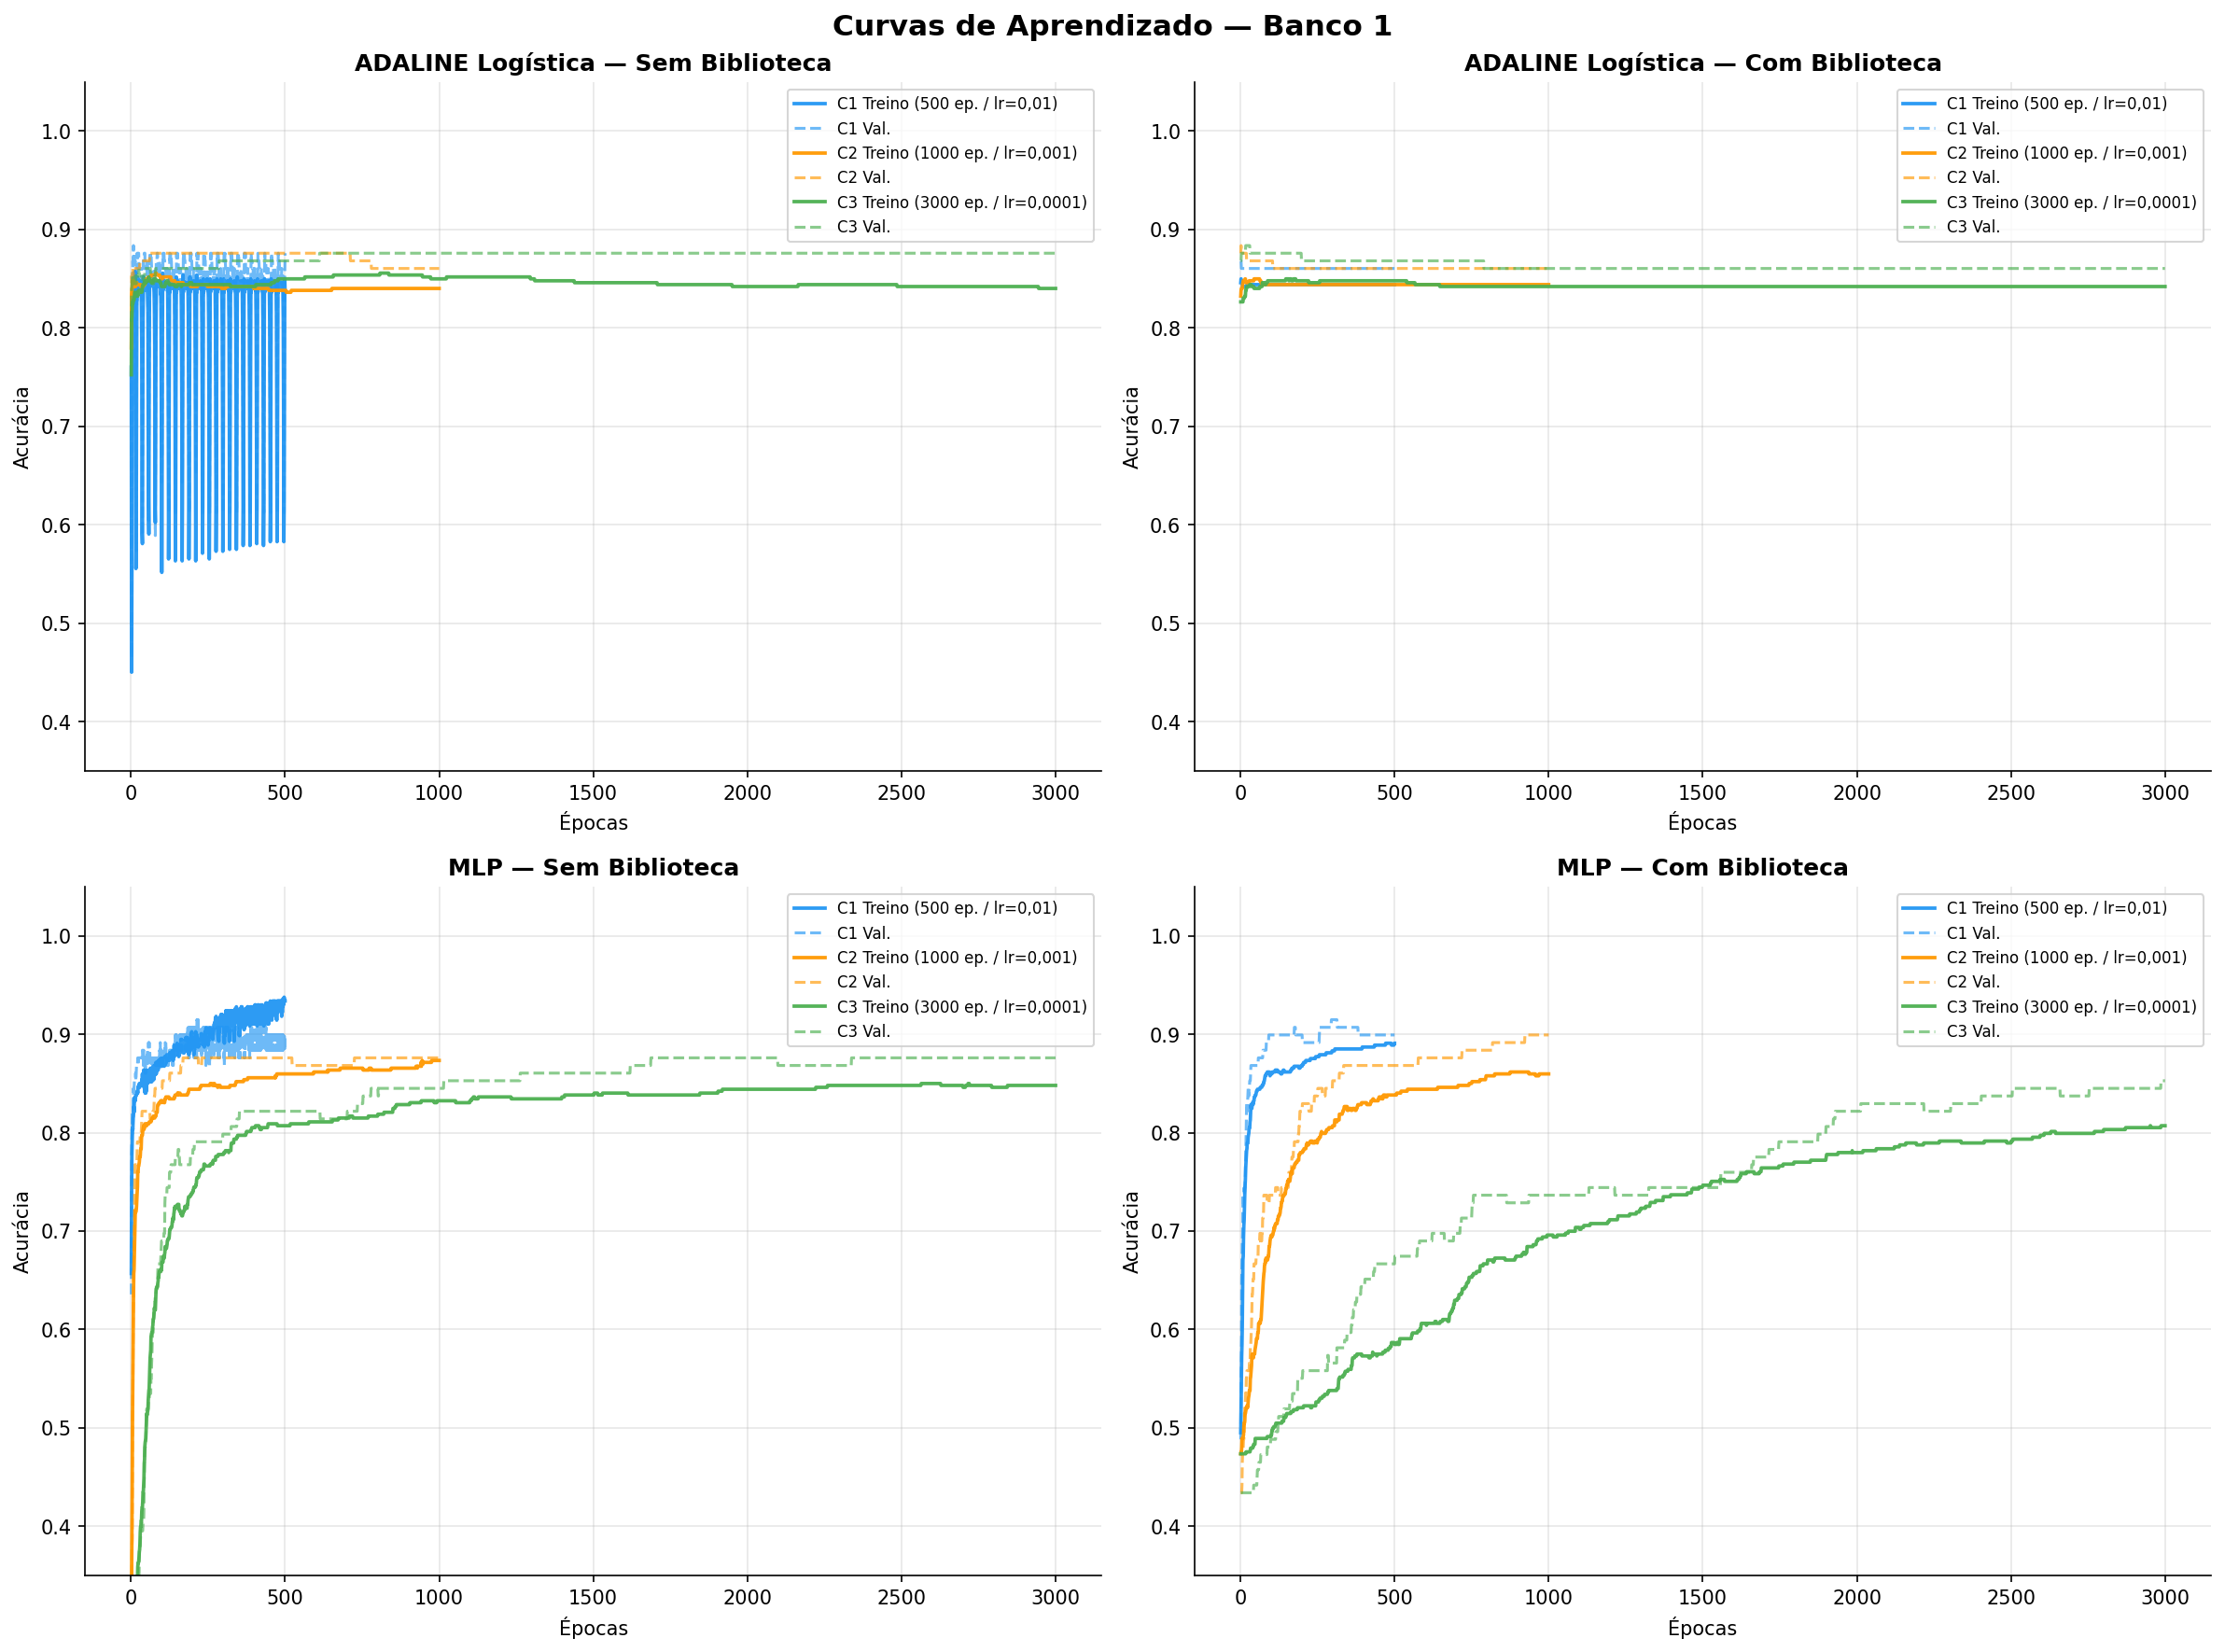
\includegraphics[width=\textwidth]{figuras/resultados/03_curvas_aprendizado_banco1.png}
\fonte{Elaborado pelo autor.}
\end{figure}

As curvas de aprendizado da Figura~\ref{fig:curvas_banco1} permitem observar o comportamento dinâmico de cada modelo ao longo das épocas. No painel do ADALINE NumPy, a configuração C1 exibe oscilações marcantes nas primeiras 500 épocas: a taxa de aprendizado elevada ($\eta = 0{,}01$) faz com que as atualizações de peso sejam grandes, provocando saltos na função de custo a cada época, comportamento característico do gradiente descendente em lote com taxa excessiva \cite{silva2016}. As configurações C2 e C3 convergem de forma suave, confirmando a estabilidade de taxas menores.

No painel do ADALINE Sklearn, as curvas são planas desde o início, com platô de validação atingido em menos de 200 épocas em todas as configurações, confirmando a convergência rápida do SGD.

O painel do MLP NumPy mostra progressão mais lenta mas consistente: a acurácia de treino e validação crescem juntas sem sinais de \textit{overfitting} (as curvas de treino e validação mantêm-se próximas), o que é esperado para gradiente descendente em lote que generaliza bem em conjuntos de tamanho moderado \cite{braga2007}. Já no painel do MLP Sklearn, observa-se para C3 um fenômeno típico de \textit{overfitting}: a curva de treino continua crescendo enquanto a curva de validação se estabiliza ou recua suavemente, indicando que o modelo começa a memorizar os exemplos de treino.

\subsection{Análise dos Falsos Negativos}
\label{sec:banco1_fn}

Conforme estabelecido na Seção~\ref{sec:metricas}, o Falso Negativo (FN), paciente doente classificado como saudável, representa o erro de maior impacto clínico neste contexto, pois implica a ausência de diagnóstico e tratamento em um paciente de risco. A Tabela~\ref{tab:fn_banco1} apresenta o total de FNs no conjunto de teste por modelo e configuração.

\begin{table}[H]
\centering
\caption[Falsos Negativos dos modelos no Banco 1 por configuração]{Total de Falsos Negativos (FN) dos modelos no Banco 1 por configuração de treinamento. Conjunto de teste: 276 pacientes (153 doentes / 123 saudáveis).}
\label{tab:fn_banco1}
\resizebox{\textwidth}{!}{%
\begin{tabular}{|l|c|c|c|}
\hline
\textbf{Modelo} & \textbf{C1 (500 ep., $\eta$=0,01)} & \textbf{C2 (1.000 ep., $\eta$=0,001)} & \textbf{C3 (3.000 ep., $\eta$=0,0001)} \\
\hline
ADALINE NumPy   & 28 & 21 & 20 \\
ADALINE Sklearn & 21 & 21 & 21 \\
MLP NumPy       & 27 & 16 & \textbf{15} \\
MLP Sklearn     & 18 & 20 & 35 \\
\hline
\end{tabular}}
\fonte{Elaborado pelo autor.}
\end{table}

A análise dos Falsos Negativos revela padrões distintos dos observados na acurácia, destacando a importância de não utilizar uma única métrica como critério de avaliação em aplicações clínicas \cite{braga2007}.

O ADALINE NumPy reduziu seus FNs progressivamente: 28 (C1) → 21 (C2) → 20 (C3). Esse comportamento é coerente com a melhora gradual da acurácia e com o fato de que a fronteira de decisão do ADALINE, ao ajustar os pesos, desloca-se em direção a uma região mais equilibrada entre sensibilidade e especificidade. Em 20 FNs, isso representa 13,07\% dos 153 pacientes doentes do conjunto de teste, um erro ainda clinicamente significativo, mas que reflete a limitação natural de um modelo linear em um problema com 35 características binárias.

O ADALINE Sklearn apresentou o comportamento mais rígido: 21 FNs em \textit{todas as configurações}, sem variação alguma. Esse resultado é notável: independentemente de se treinarem 500, 1.000 ou 3.000 épocas, e com taxas de aprendizado que variam 100 vezes (de 0,01 a 0,0001), o modelo sempre classificou incorretamente os mesmos 21 pacientes. Isso indica que o SGD atingiu um mínimo de custo específico que não é alterado por mudanças nos hiperparâmetros testados, o que pode ser interpretado como robustez do ponto de convergência, mas também como insensibilidade ao espaço de busca definido pelas configurações C1--C3.

O MLP NumPy obteve os melhores resultados clínicos do Banco 1: 27 FNs em C1, reduzindo para 16 em C2 e atingindo o mínimo de 15 FNs em C3. Esse progresso gradual é particularmente relevante porque a acurácia também melhorou no mesmo sentido (82,97\% → 87,68\%), o que significa que o modelo ganhou em ambas as dimensões simultaneamente. Com 15 FNs em 153 doentes, a sensibilidade alcança 90,20\%, significando que 9 em cada 10 pacientes doentes são corretamente identificados como doentes na configuração C3.

O MLP Sklearn demonstrou o comportamento mais problemático clinicamente: embora tenha iniciado com bons resultados em C1 (18 FNs), degradou-se progressivamente para 20 em C2 e chegou ao pior resultado do Banco 1 com 35 FNs em C3. Esse número representa 22,88\% dos pacientes doentes sendo classificados como saudáveis, quase um em cada quatro doentes não detectados. Esse resultado contradiz diretamente a acurácia de C1 (87,32\%) e demonstra que a otimização de acurácia global não garante minimização de FNs.

A Figura~\ref{fig:matrizes_banco1} apresenta as matrizes de confusão de todos os modelos na configuração C3 (3.000 épocas, $\eta = 0{,}0001$). Essa configuração foi adotada como referência de visualização por ser aquela em que as diferenças de comportamento clínico entre os modelos se manifestam de forma mais acentuada: em particular, a degradação do MLP Sklearn, com 35 Falsos Negativos em C3 contra 18 em C1, torna-se visível nas matrizes e faz da comparação entre arquiteturas nessa configuração a mais informativa dentre as três estudadas.

\begin{figure}[H]
\centering
\caption[Matrizes de confusão dos modelos, Banco 1, configuração C3.]{Matrizes de confusão dos quatro modelos no Banco 1, configuração C3 (3.000 épocas, $\eta$ = 0,0001).}
\label{fig:matrizes_banco1}
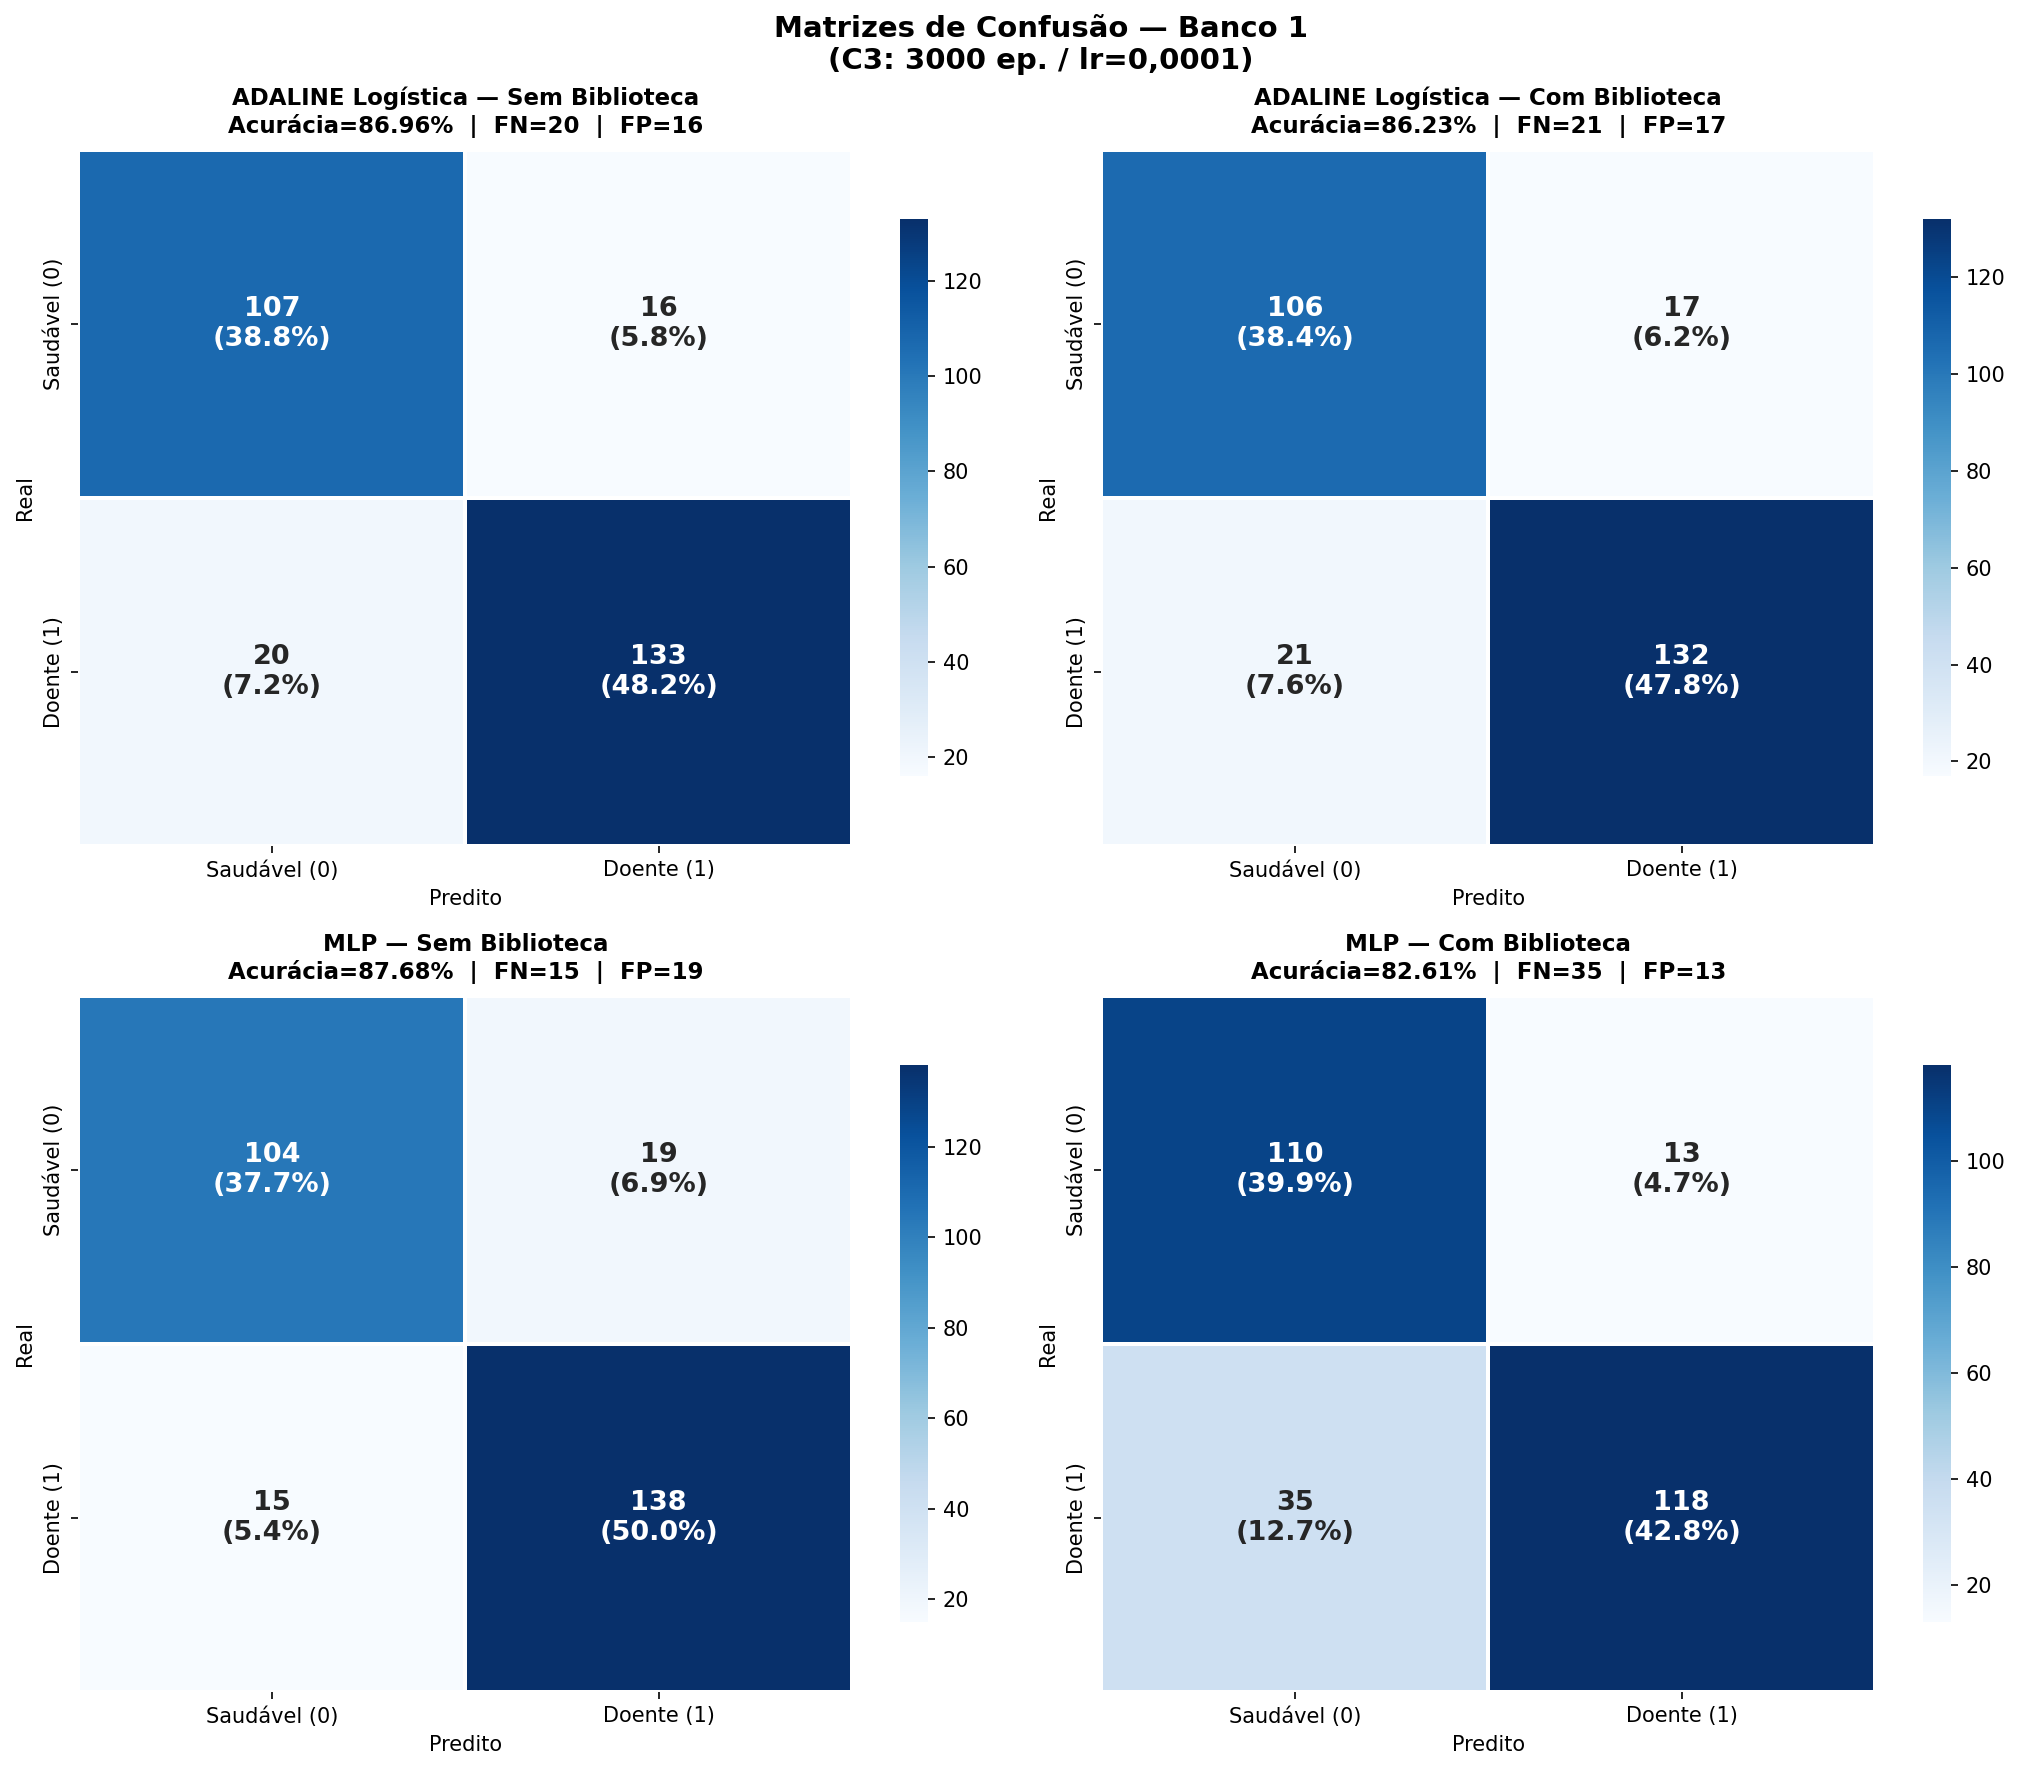
\includegraphics[width=\textwidth]{figuras/resultados/07_matrizes_confusao_banco1.png}
\fonte{Elaborado pelo autor.}
\end{figure}

A partir das matrizes de confusão da Figura~\ref{fig:matrizes_banco1} e dos valores de VP, VN, FP e FN, é possível calcular as métricas complementares de sensibilidade, especificidade e precisão. A Tabela~\ref{tab:metricas_banco1_c3} consolida esses valores para C3.

\begin{table}[H]
\centering
\caption{Métricas de avaliação dos modelos no Banco 1, configuração C3. Conjunto de teste: 276 pacientes.}
\label{tab:metricas_banco1_c3}
\begin{tabular}{|l|c|c|c|c|c|c|c|}
\hline
\textbf{Modelo} & \textbf{VP} & \textbf{VN} & \textbf{FP} & \textbf{FN} & \textbf{Sensib.} & \textbf{Especif.} & \textbf{Precisão} \\
\hline
ADALINE NumPy   & 133 & 107 & 16 & 20 & 86,93\% & 86,99\% & 89,26\% \\
ADALINE Sklearn & 132 & 106 & 17 & 21 & 86,27\% & 86,18\% & 88,59\% \\
MLP NumPy       & 138 & 104 & 19 & 15 & \textbf{90,20\%} & 84,55\% & 87,90\% \\
MLP Sklearn     & 118 & 110 & 13 & 35 & 77,12\% & \textbf{89,43\%} & 90,08\% \\
\hline
\end{tabular}
\fonte{Elaborado pelo autor.}
\vspace*{-\baselineskip}
\end{table}

A Tabela~\ref{tab:metricas_banco1_c3} evidencia um contraste fundamental entre os modelos em C3. O MLP NumPy atingiu a maior sensibilidade (90,20\%), identificando corretamente 138 dos 153 pacientes doentes, resultado clinicamente mais relevante. O MLP Sklearn, por sua vez, apresentou a maior especificidade (89,43\%) e precisão (90,08\%), mas ao custo de uma sensibilidade muito inferior (77,12\%) e do maior número de FNs (35). Isso revela que o MLP Sklearn em C3 aprendeu a ser conservador na predição de doença, classificando mais pacientes como saudáveis, o que reduz os FPs e aumenta a especificidade, mas eleva os FNs a níveis clinicamente inaceitáveis. Os dois modelos ADALINE apresentaram sensibilidade e especificidade equilibradas (ambas próximas de 87\%), comportamento coerente com a natureza simétrica da função logística e com a convergência estável da regra delta.

\subsection{Convergência do Erro de Treinamento}
\label{sec:banco1_convergencia}

A Figura~\ref{fig:convergencia_banco1} apresenta a evolução do Erro Quadrático Médio (MSE) ao longo das épocas de treinamento para os quatro modelos no Banco 1, permitindo comparar a velocidade de convergência e a estabilidade de cada abordagem.

\begin{figure}[H]
\centering
\caption{Convergência do Erro Quadrático Médio (MSE) por época nos quatro modelos, Banco 1.}
\label{fig:convergencia_banco1}
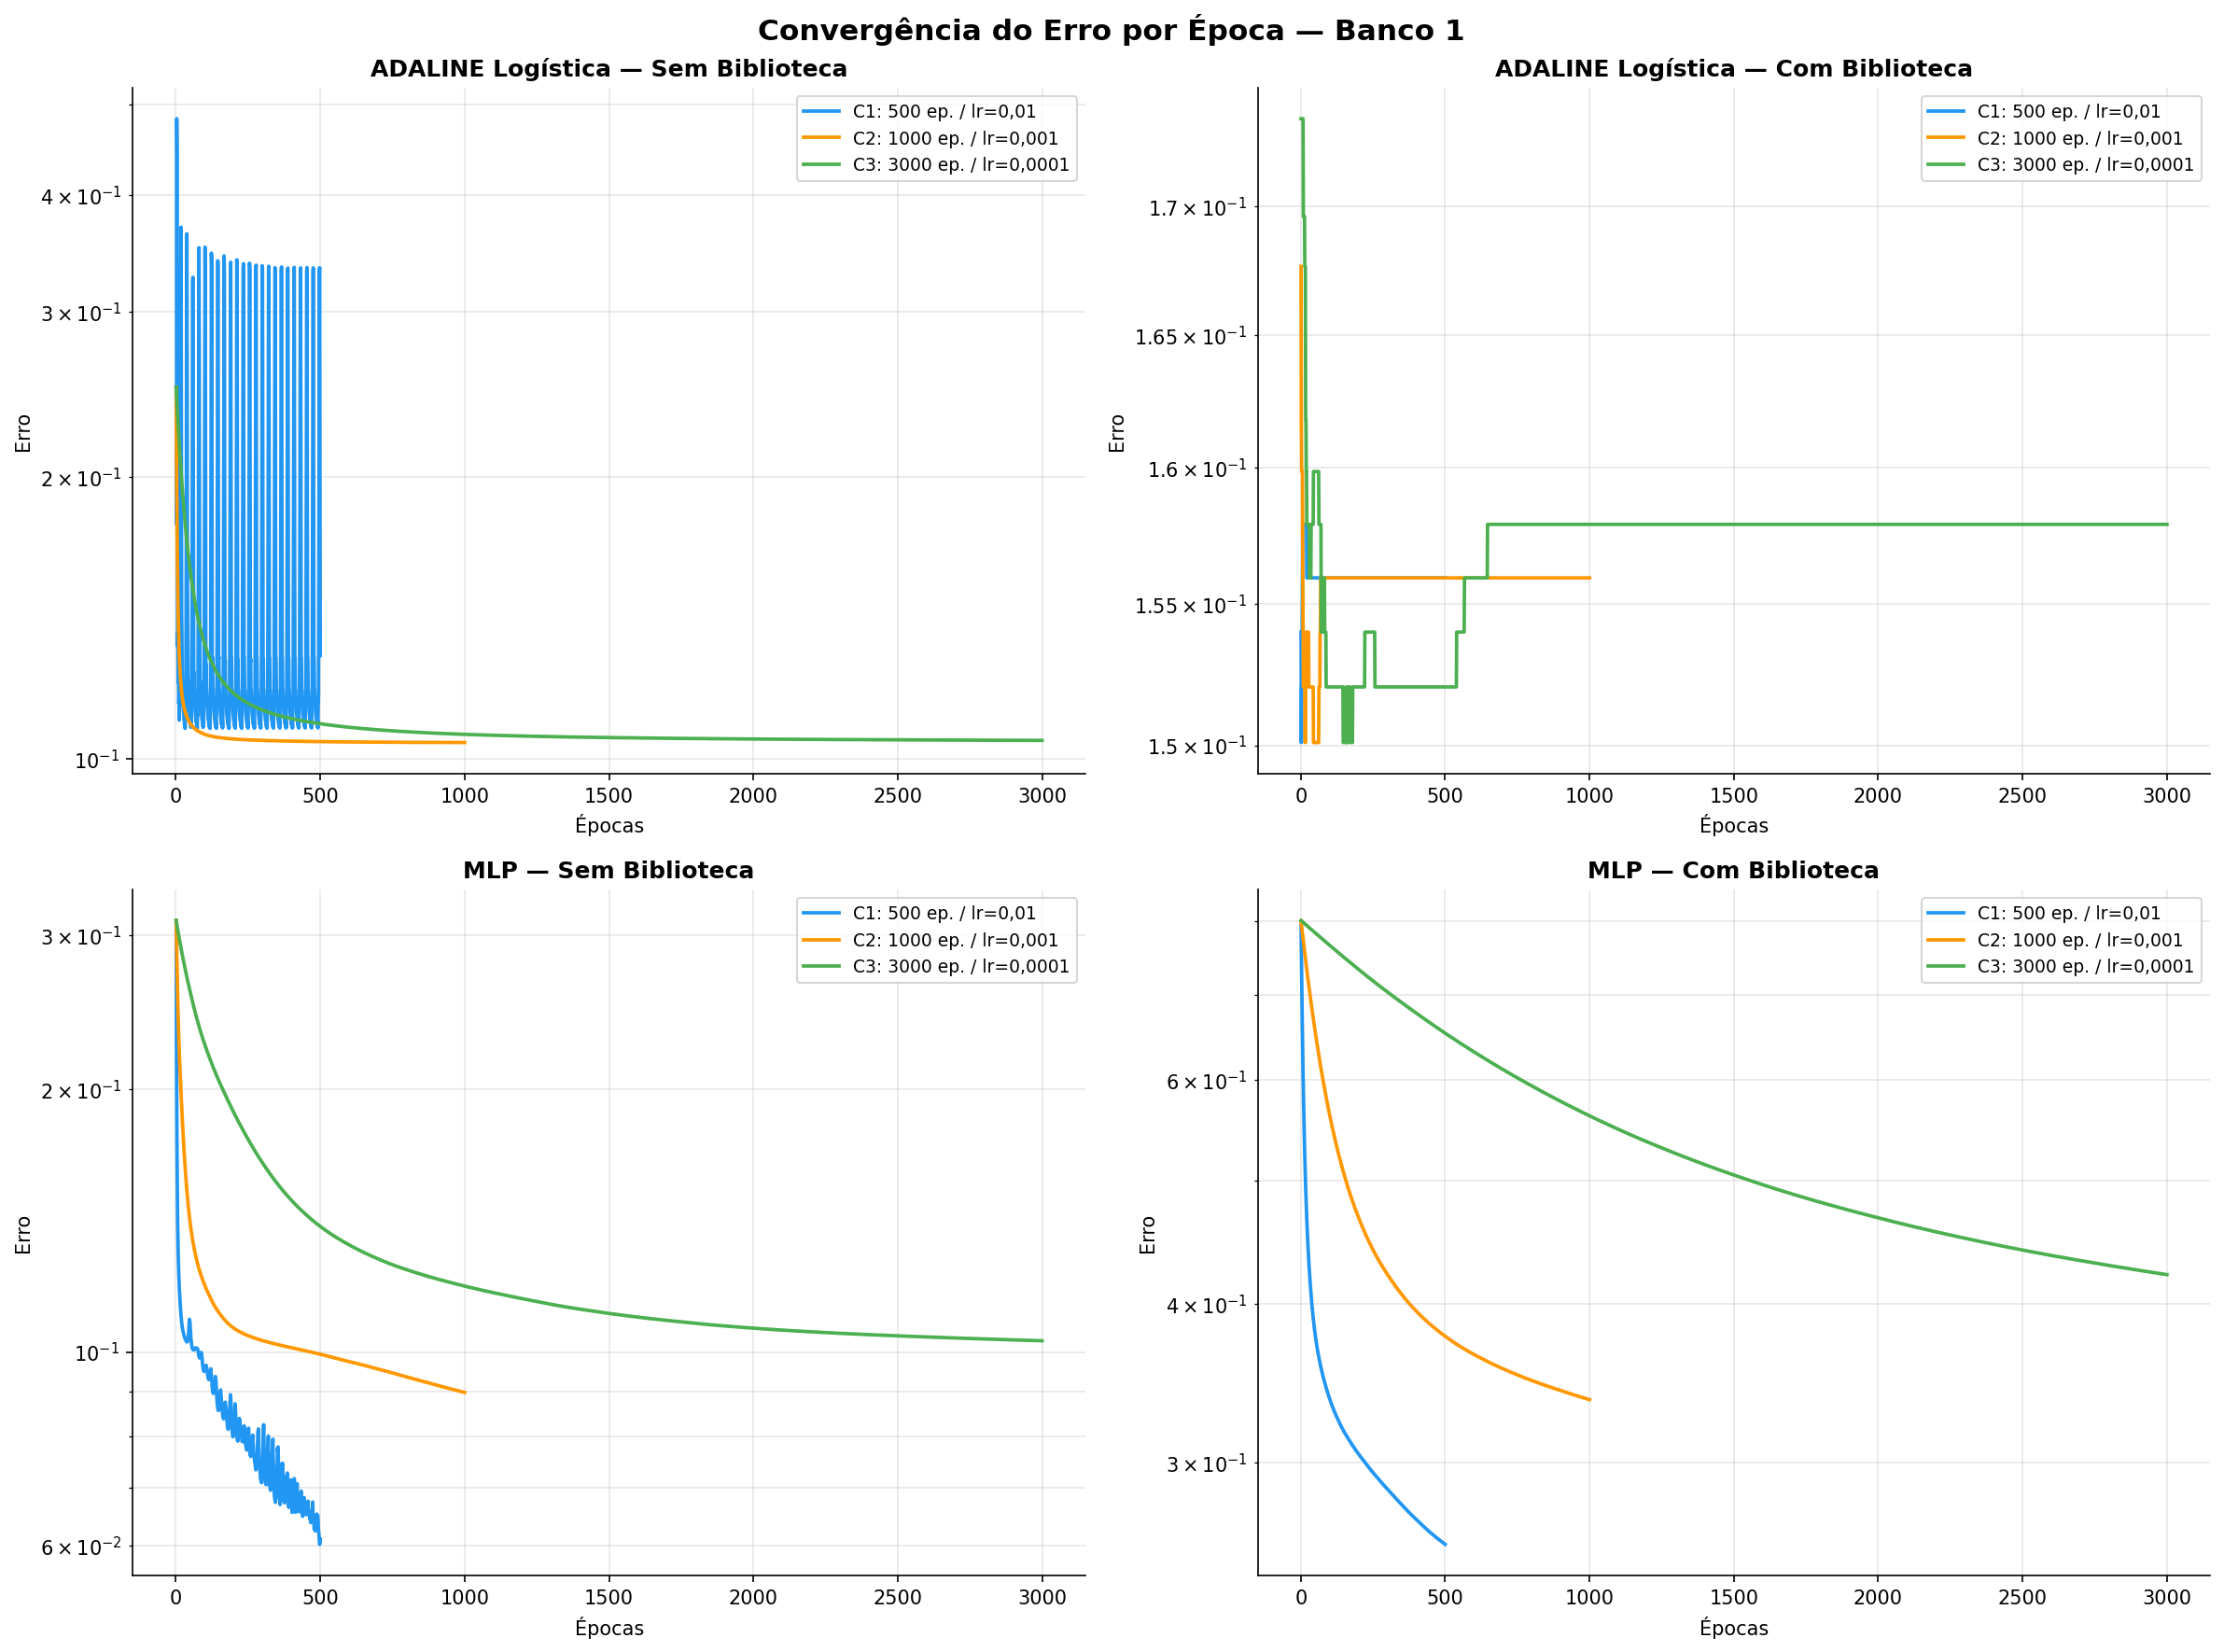
\includegraphics[width=\textwidth]{figuras/resultados/05_convergencia_erro_banco1.png}
\fonte{Elaborado pelo autor.}
\end{figure}

A Figura~\ref{fig:convergencia_banco1} ilustra a evolução do MSE de treinamento ao longo das épocas. Dois comportamentos contrastantes são imediatamente visíveis.

No painel do ADALINE NumPy, a configuração C1 ($\eta = 0{,}01$) exibe oscilações de grande amplitude nas primeiras épocas, com o erro chegando a valores próximos de $4 \times 10^{-1}$ antes de decair. Essas oscilações decorrem diretamente da taxa de aprendizado elevada em combinação com o gradiente calculado sobre todo o conjunto de treinamento (modo lote): quando $\eta$ é grande, cada passo de gradiente pode ultrapassar o mínimo da função de custo, fazendo o erro oscilar antes de convergir. As configurações C2 e C3 convergem suavemente e de forma monotônica, confirmando que taxas menores produzem trajetórias mais estáveis, ainda que mais lentas \cite{silva2016}.

No painel do ADALINE Sklearn, as três curvas são planas e estacionárias desde o início, coerentes com o comportamento de acurácia observado na Seção~\ref{sec:banco1_acuracia}.

Os painéis do MLP NumPy e MLP Sklearn mostram curvas de convergência mais lentas e com patamares distintos. Para o MLP NumPy, as três configurações apresentam convergência suave e monotônica, com C1 atingindo erro maior (ainda convergindo mais lentamente por ter apenas 500 épocas), C2 chegando a um nível intermediário e C3 atingindo o menor erro final, consistente com os melhores resultados de acurácia e FNs em C3. Para o MLP Sklearn, a curva de C3 apresenta erro decrescente ao longo das 3.000 épocas sem sinais de estabilização, o que, combinado com a acurácia de validação estacionária (Figura~\ref{fig:curvas_banco1}), é sinal inequívoco de \textit{overfitting}: o modelo está reduzindo o erro de treino enquanto a capacidade de generalização piora \cite{dsa2022}.

\section{Banco 2 --- Heart Failure Clinical Records}
\label{sec:resultados_banco2}

O Banco 2 contém 299 registros de pacientes com insuficiência cardíaca diagnosticada, com objetivo de prognóstico de mortalidade (\textit{DEATH\_EVENT}). Após a divisão estratificada, o conjunto de teste compreende 90 pacientes: 61 sobreviventes (67,8\%) e 29 óbitos (32,2\%). O volume significativamente menor (299 versus 918 do Banco 1), o desequilíbrio de classes mais acentuado (33\% versus 45\% de positivos) e a natureza mais complexa do objetivo preditivo, prognóstico de óbito em vez de triagem diagnóstica, tornam este banco intrinsecamente mais desafiador \cite{chicco2020}.

\subsection{Acurácia por Configuração de Treinamento}
\label{sec:banco2_acuracia}

A Tabela~\ref{tab:acuracia_banco2} apresenta a acurácia percentual de cada modelo nas três configurações de treinamento para o Banco 2. O padrão de desempenho difere fundamentalmente do Banco 1: as acurácias globais são menores e as trajetórias dos modelos MLP ao longo das configurações são inversas ao comportamento observado anteriormente, com degradação progressiva do desempenho à medida que o treinamento se estende.

\begin{table}[H]
\centering
\caption{Acurácia (\%) dos modelos no Banco 2 por configuração de treinamento.}
\label{tab:acuracia_banco2}
\resizebox{\textwidth}{!}{%
\begin{tabular}{|l|c|c|c|}
\hline
\textbf{Modelo} & \textbf{C1 (500 ep., $\eta$=0,01)} & \textbf{C2 (1.000 ep., $\eta$=0,001)} & \textbf{C3 (3.000 ep., $\eta$=0,0001)} \\
\hline
ADALINE NumPy   & 68,89\% & 72,22\% & \textbf{75,56\%} \\
ADALINE Sklearn & 68,89\% & 68,89\% & 68,89\% \\
MLP NumPy       & \textbf{78,89\%} & 75,56\% & 71,11\% \\
MLP Sklearn     & 73,33\% & 68,89\% & 63,33\% \\
\hline
\end{tabular}}
\fonte{Elaborado pelo autor.}
\end{table}

O ADALINE NumPy é o único modelo cujo desempenho melhora monotonicamente: 68,89\% → 72,22\% → 75,56\%. Esse comportamento reflete a estabilidade do gradiente descendente em lote com taxas conservadoras em conjuntos pequenos, o modelo ajusta a fronteira linear lentamente mas sem instabilidade \cite{silva2016}.

O ADALINE Sklearn repetiu o comportamento de rigidez observado no Banco 1, mas de forma ainda mais extrema: acurácia idêntica de 68,89\% em \textit{todas as três configurações}, sem qualquer variação. Em um conjunto de 90 pacientes de teste, isso equivale a exatamente 62 classificações corretas em todas as situações. O SGD converge para um mínimo específico nas primeiras épocas e permanece estacionário, insensível a qualquer ajuste de hiperparâmetros dentro do espaço testado. Esse comportamento, que no Banco 1 poderia ser interpretado como convergência robusta, no Banco 2 é mais indicativo de uma limitação: o modelo está preso em uma solução subótima que não consegue sair \cite{pedregosa2011}.

O MLP NumPy apresentou o resultado inverso ao esperado: a melhor configuração foi C1 (78,89\%), e o desempenho degradou progressivamente em C2 (75,56\%) e C3 (71,11\%). Esse fenômeno é um caso claro de \textit{overfitting} induzido por treinamento excessivo em um conjunto de dados pequeno: com apenas 167 exemplos efetivos de treinamento (correspondentes a 80\% dos 209 pacientes do conjunto de treino obtido pela divisão 70/30), 3.000 épocas representam 3.000 passagens completas pelo conjunto de treino de 167 exemplos, número excessivo para um conjunto tão pequeno com gradiente descendente em lote. O modelo passa a memorizar os exemplos individuais de treino em vez de aprender padrões generalizáveis \cite{braga2007}.

O MLP Sklearn apresentou a degradação mais severa de todos: 73,33\% em C1, caindo para 68,89\% em C2 e chegando ao mínimo de 63,33\% em C3, a menor acurácia de todos os experimentos. O SGD com momento ($\beta = 0{,}9$), com sua velocidade acumulada que continua impulsionando os parâmetros mesmo em fases avançadas do treinamento, é particularmente suscetível a \textit{overfitting} em datasets pequenos: sem dados suficientes para regularizar o aprendizado, a velocidade acumulada ajusta os pesos excessivamente aos exemplos de treino \cite{dsa2022}.

\begin{figure}[H]
\centering
\caption{Curvas de aprendizado (acurácia de treino e validação) dos quatro modelos no Banco 2 para as três configurações de treinamento.}
\label{fig:curvas_banco2}
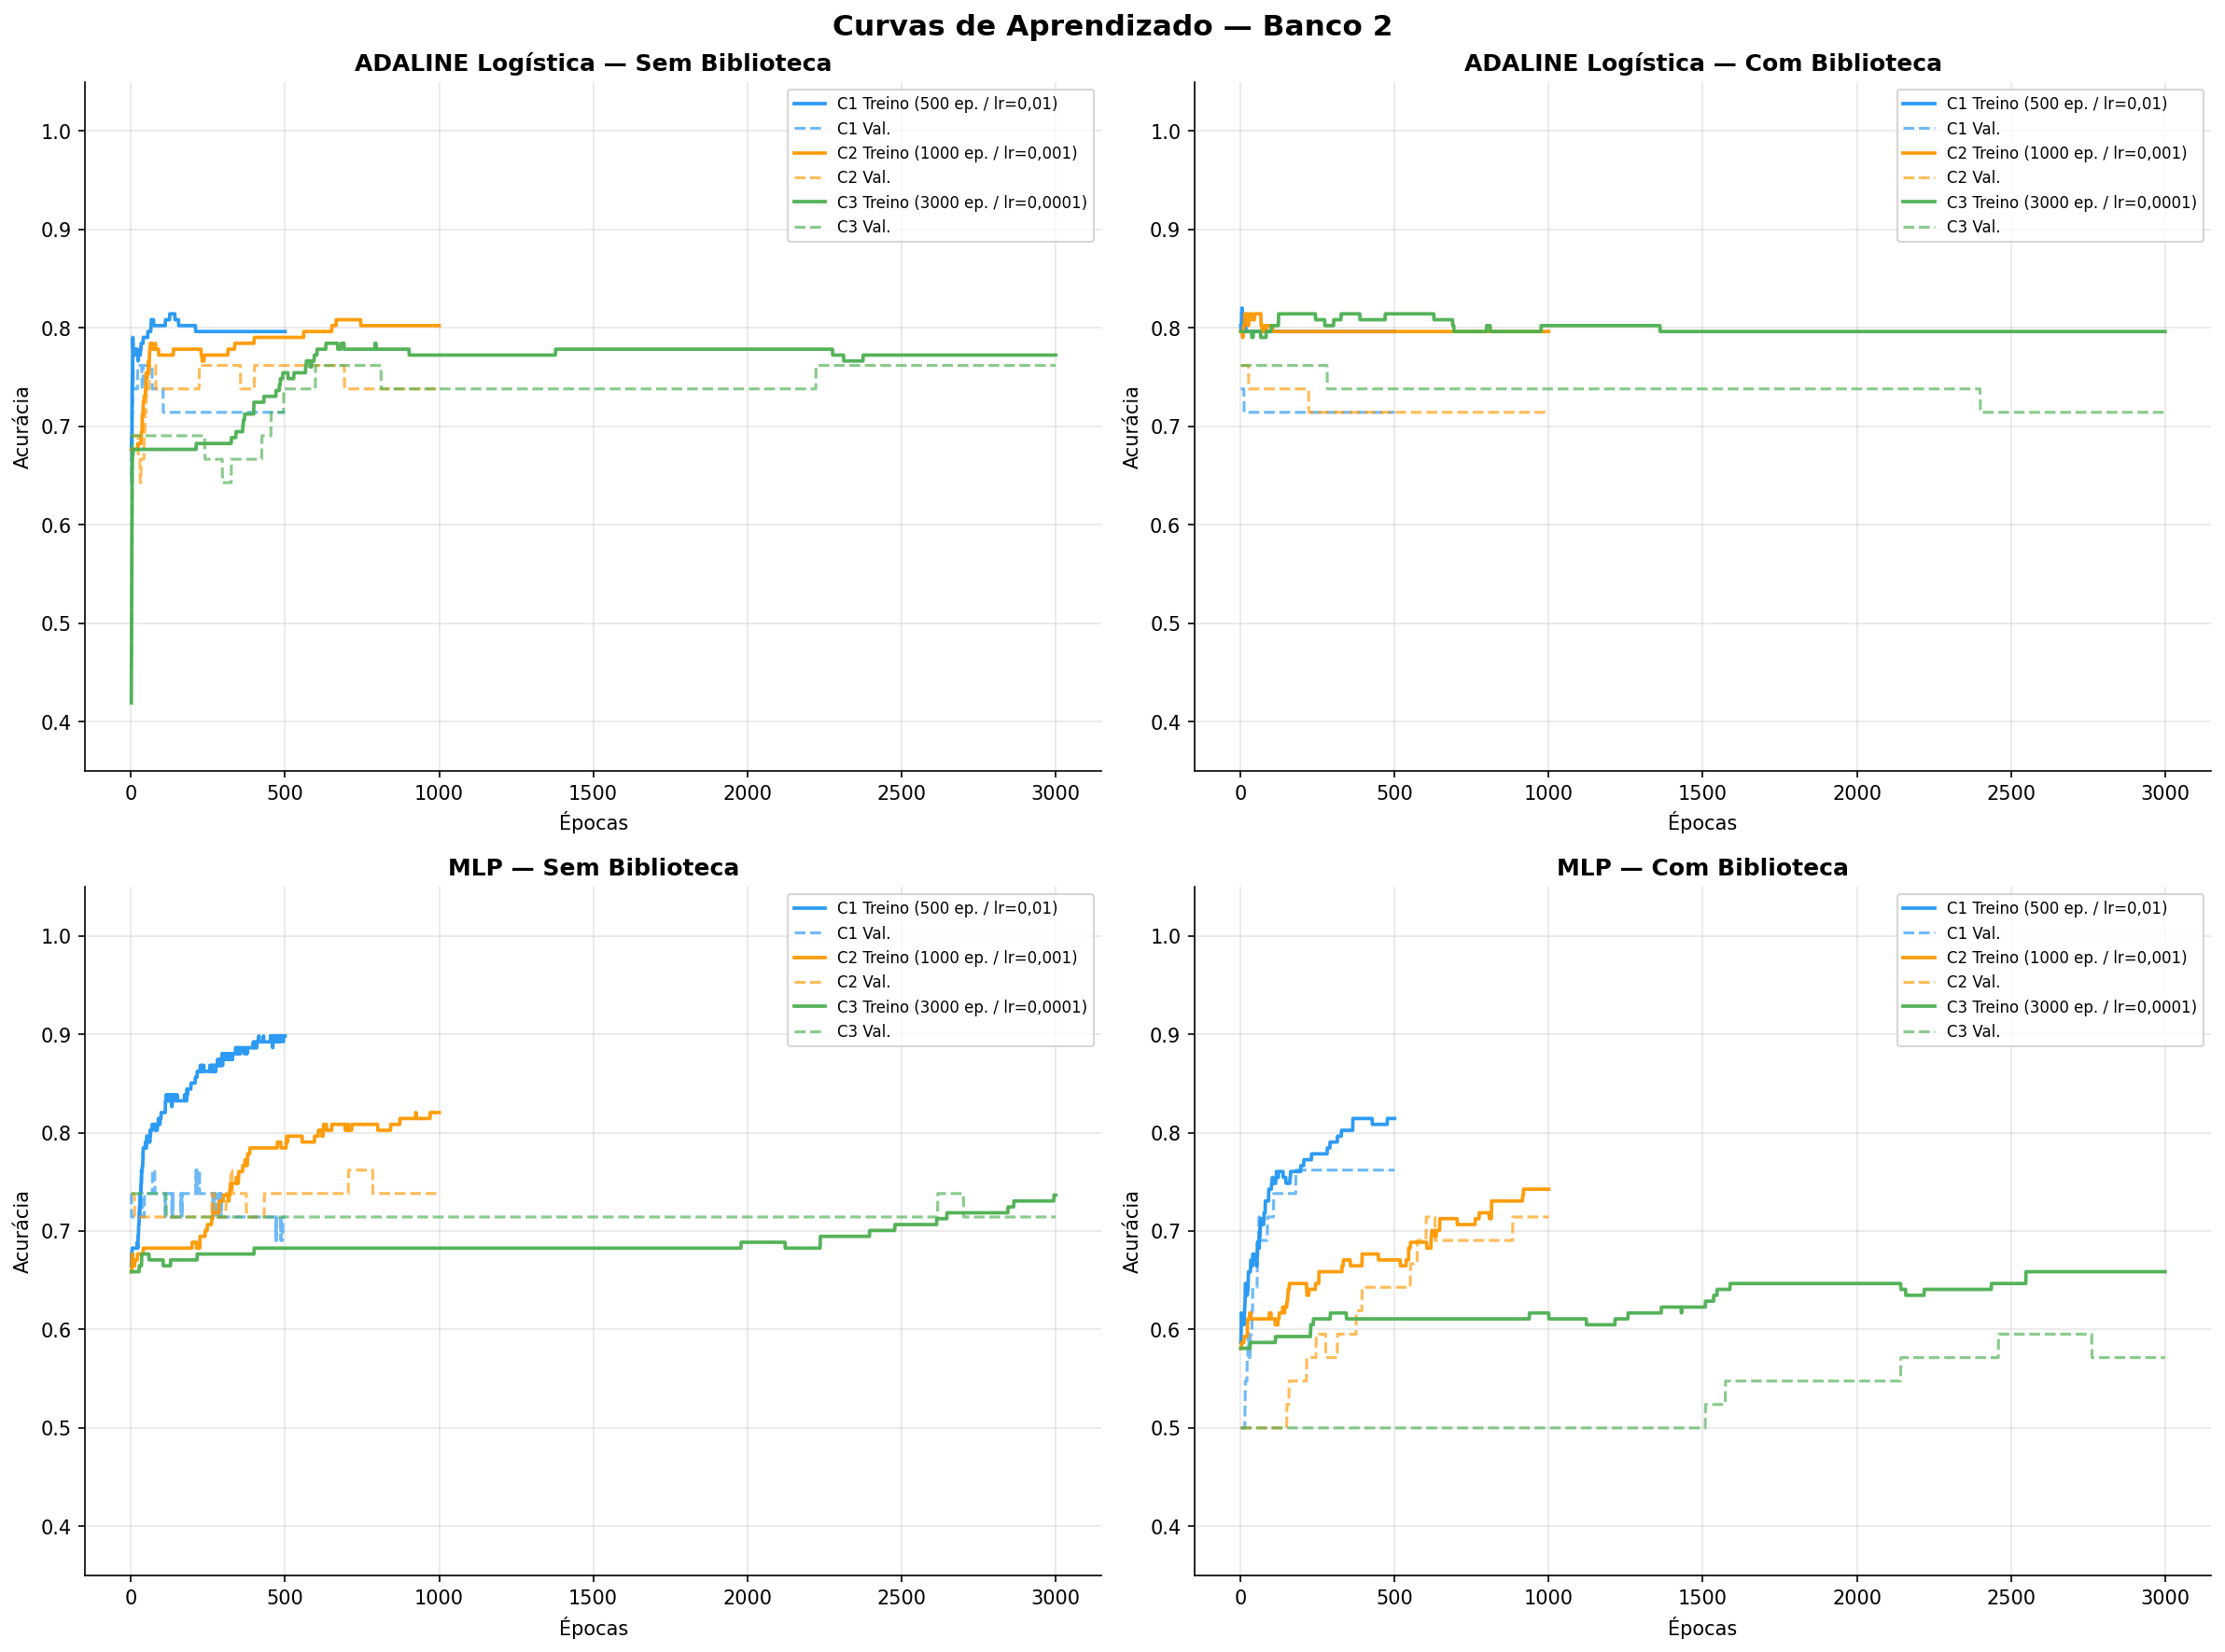
\includegraphics[width=\textwidth]{figuras/resultados/04_curvas_aprendizado_banco2.png}
\fonte{Elaborado pelo autor.}
\end{figure}

A Figura~\ref{fig:curvas_banco2} evidencia o \textit{overfitting} dos modelos MLP: em C3, a acurácia de treino continua crescendo enquanto a de validação oscila ou recua, com divergência especialmente pronunciada no MLP Sklearn. O comportamento escalonado do ADALINE Sklearn confirma a rigidez do SGD.

\subsection{Análise dos Falsos Negativos}
\label{sec:banco2_fn}

Neste banco, em que a classe positiva corresponde aos óbitos, apenas 29 dos 90 pacientes do conjunto de teste, a análise dos Falsos Negativos assume especial relevância clínica. Cada FN representa um paciente que veio a óbito mas foi classificado como sobrevivente pelo modelo, erro que poderia implicar a ausência de intervenção terapêutica em tempo oportuno. A Tabela~\ref{tab:fn_banco2} apresenta o total de FNs por modelo e configuração.

\begin{table}[H]
\centering
\caption[Falsos Negativos dos modelos no Banco 2 por configuração]{Total de Falsos Negativos (FN) dos modelos no Banco 2 por configuração de treinamento. Conjunto de teste: 90 pacientes (29 óbitos / 61 sobreviventes).}
\label{tab:fn_banco2}
\resizebox{\textwidth}{!}{%
\begin{tabular}{|l|c|c|c|}
\hline
\textbf{Modelo} & \textbf{C1 (500 ep., $\eta$=0,01)} & \textbf{C2 (1.000 ep., $\eta$=0,001)} & \textbf{C3 (3.000 ep., $\eta$=0,0001)} \\
\hline
ADALINE NumPy   & 17 & 17 & 16 \\
ADALINE Sklearn & 17 & 17 & 17 \\
MLP NumPy       & \textbf{9}  & 14 & 23 \\
MLP Sklearn     & 18 & 17 & \textbf{8} \\
\hline
\end{tabular}}
\fonte{Elaborado pelo autor.}
\end{table}

A Tabela~\ref{tab:fn_banco2} revela um dos resultados mais intrigantes de todo o trabalho: o MLP Sklearn em C3, que apresentou a \textit{pior} acurácia (63,33\%), produziu simultaneamente o \textit{menor} número de Falsos Negativos (8 FNs). Aparentemente contraditório, esse resultado é explicado pela análise das matrizes de confusão (Figura~\ref{fig:matrizes_banco2}): o modelo aprendeu a classificar uma proporção elevada de pacientes como doentes (\textit{DEATH\_EVENT} = 1), o que reduz os FNs ao custo de inflar dramaticamente os Falsos Positivos. Trata-se de uma troca desfavorável para uso clínico, pois pacientes saudáveis são alarmados desnecessariamente, mas que ilustra como a escolha da métrica de avaliação principal influencia a interpretação do desempenho de um modelo \cite{braga2007}.

O MLP NumPy em C1 obteve o melhor equilíbrio entre acurácia e FNs no Banco 2: 78,89\% de acurácia e apenas 9 FNs, representando 31,03\% de falhas na detecção de óbitos. Isso equivale a uma sensibilidade de 68,97\%, o melhor resultado geral deste banco de dados. A degradação progressiva do MLP NumPy em C2 (14 FNs) e C3 (23 FNs) confirma o \textit{overfitting}: à medida que o modelo se especializa nos exemplos de treino, começa a errar em exemplos de teste que não foram memorizados, e por ser a classe de óbito a minoria (33\%), os erros tendem a recair desproporcionalmente sobre ela.

Os modelos ADALINE mantiveram FNs estáveis em torno de 16--17 em todas as configurações, coerente com a fronteira de decisão linear que não se altera significativamente entre as configurações. Com 17 FNs em 29 óbitos, a sensibilidade do ADALINE Sklearn é de 41,38\%, diagnosticando corretamente apenas 2 em cada 5 pacientes que vieram a óbito. Embora este número seja clinicamente preocupante, ele reflete a dificuldade inerente do problema: prever óbito em pacientes com insuficiência cardíaca a partir de dados clínicos tabulares e binários é uma tarefa com alto grau de incerteza, e a acurácia de 75,56\% atingida pelo ADALINE NumPy em C3, com apenas 16 FNs, representa o melhor compromisso entre confiabilidade global e detecção de casos críticos neste banco \cite{chicco2020}.

Dado que a configuração C1 representa o melhor desempenho geral do Banco 2, a Tabela~\ref{tab:metricas_banco2_c1} detalha as métricas consolidadas para essa configuração, derivadas das contagens de VP, VN, FP e FN calculadas a partir da acurácia e dos FNs apresentados nas Tabelas~\ref{tab:acuracia_banco2} e \ref{tab:fn_banco2}.

\begin{table}[H]
\centering
\caption{Métricas de avaliação dos modelos no Banco 2, configuração C1. Conjunto de teste: 90 pacientes (29 óbitos / 61 sobreviventes).}
\label{tab:metricas_banco2_c1}
\begin{tabular}{|l|c|c|c|c|c|c|c|}
\hline
\textbf{Modelo} & \textbf{VP} & \textbf{VN} & \textbf{FP} & \textbf{FN} & \textbf{Sensib.} & \textbf{Especif.} & \textbf{Precisão} \\
\hline
ADALINE NumPy   & 12 & 50 & 11 & 17 & 41,38\% & 81,97\% & 52,17\% \\
ADALINE Sklearn & 12 & 50 & 11 & 17 & 41,38\% & 81,97\% & 52,17\% \\
MLP NumPy       & 20 & 51 & 10 &  9 & \textbf{68,97\%} & 83,61\% & 66,67\% \\
MLP Sklearn     & 11 & 55 &  6 & 18 & 37,93\% & \textbf{90,16\%} & 64,71\% \\
\hline
\end{tabular}
\fonte{Elaborado pelo autor.}
\end{table}

A Tabela~\ref{tab:metricas_banco2_c1} confirma que o MLP NumPy em C1 oferece o melhor equilíbrio entre sensibilidade (68,97\%) e especificidade (83,61\%), identificando 20 dos 29 óbitos com apenas 10 falsos alarmes. O MLP Sklearn em C1, apesar de boa especificidade (90,16\%), apresenta a pior sensibilidade (37,93\%), menos de 4 em cada 10 óbitos detectados. Os dois modelos ADALINE são idênticos em C1, com sensibilidade de 41,38\% e especificidade de 81,97\%, resultado da mesma convergência atingida pelo gradiente descendente e pelo SGD nessa configuração.

\begin{figure}[H]
\centering
\caption[Matrizes de confusão dos modelos, Banco 2, configuração C3.]{Matrizes de confusão dos quatro modelos no Banco 2, configuração C3 (3.000 épocas, $\eta$ = 0,0001).}
\label{fig:matrizes_banco2}
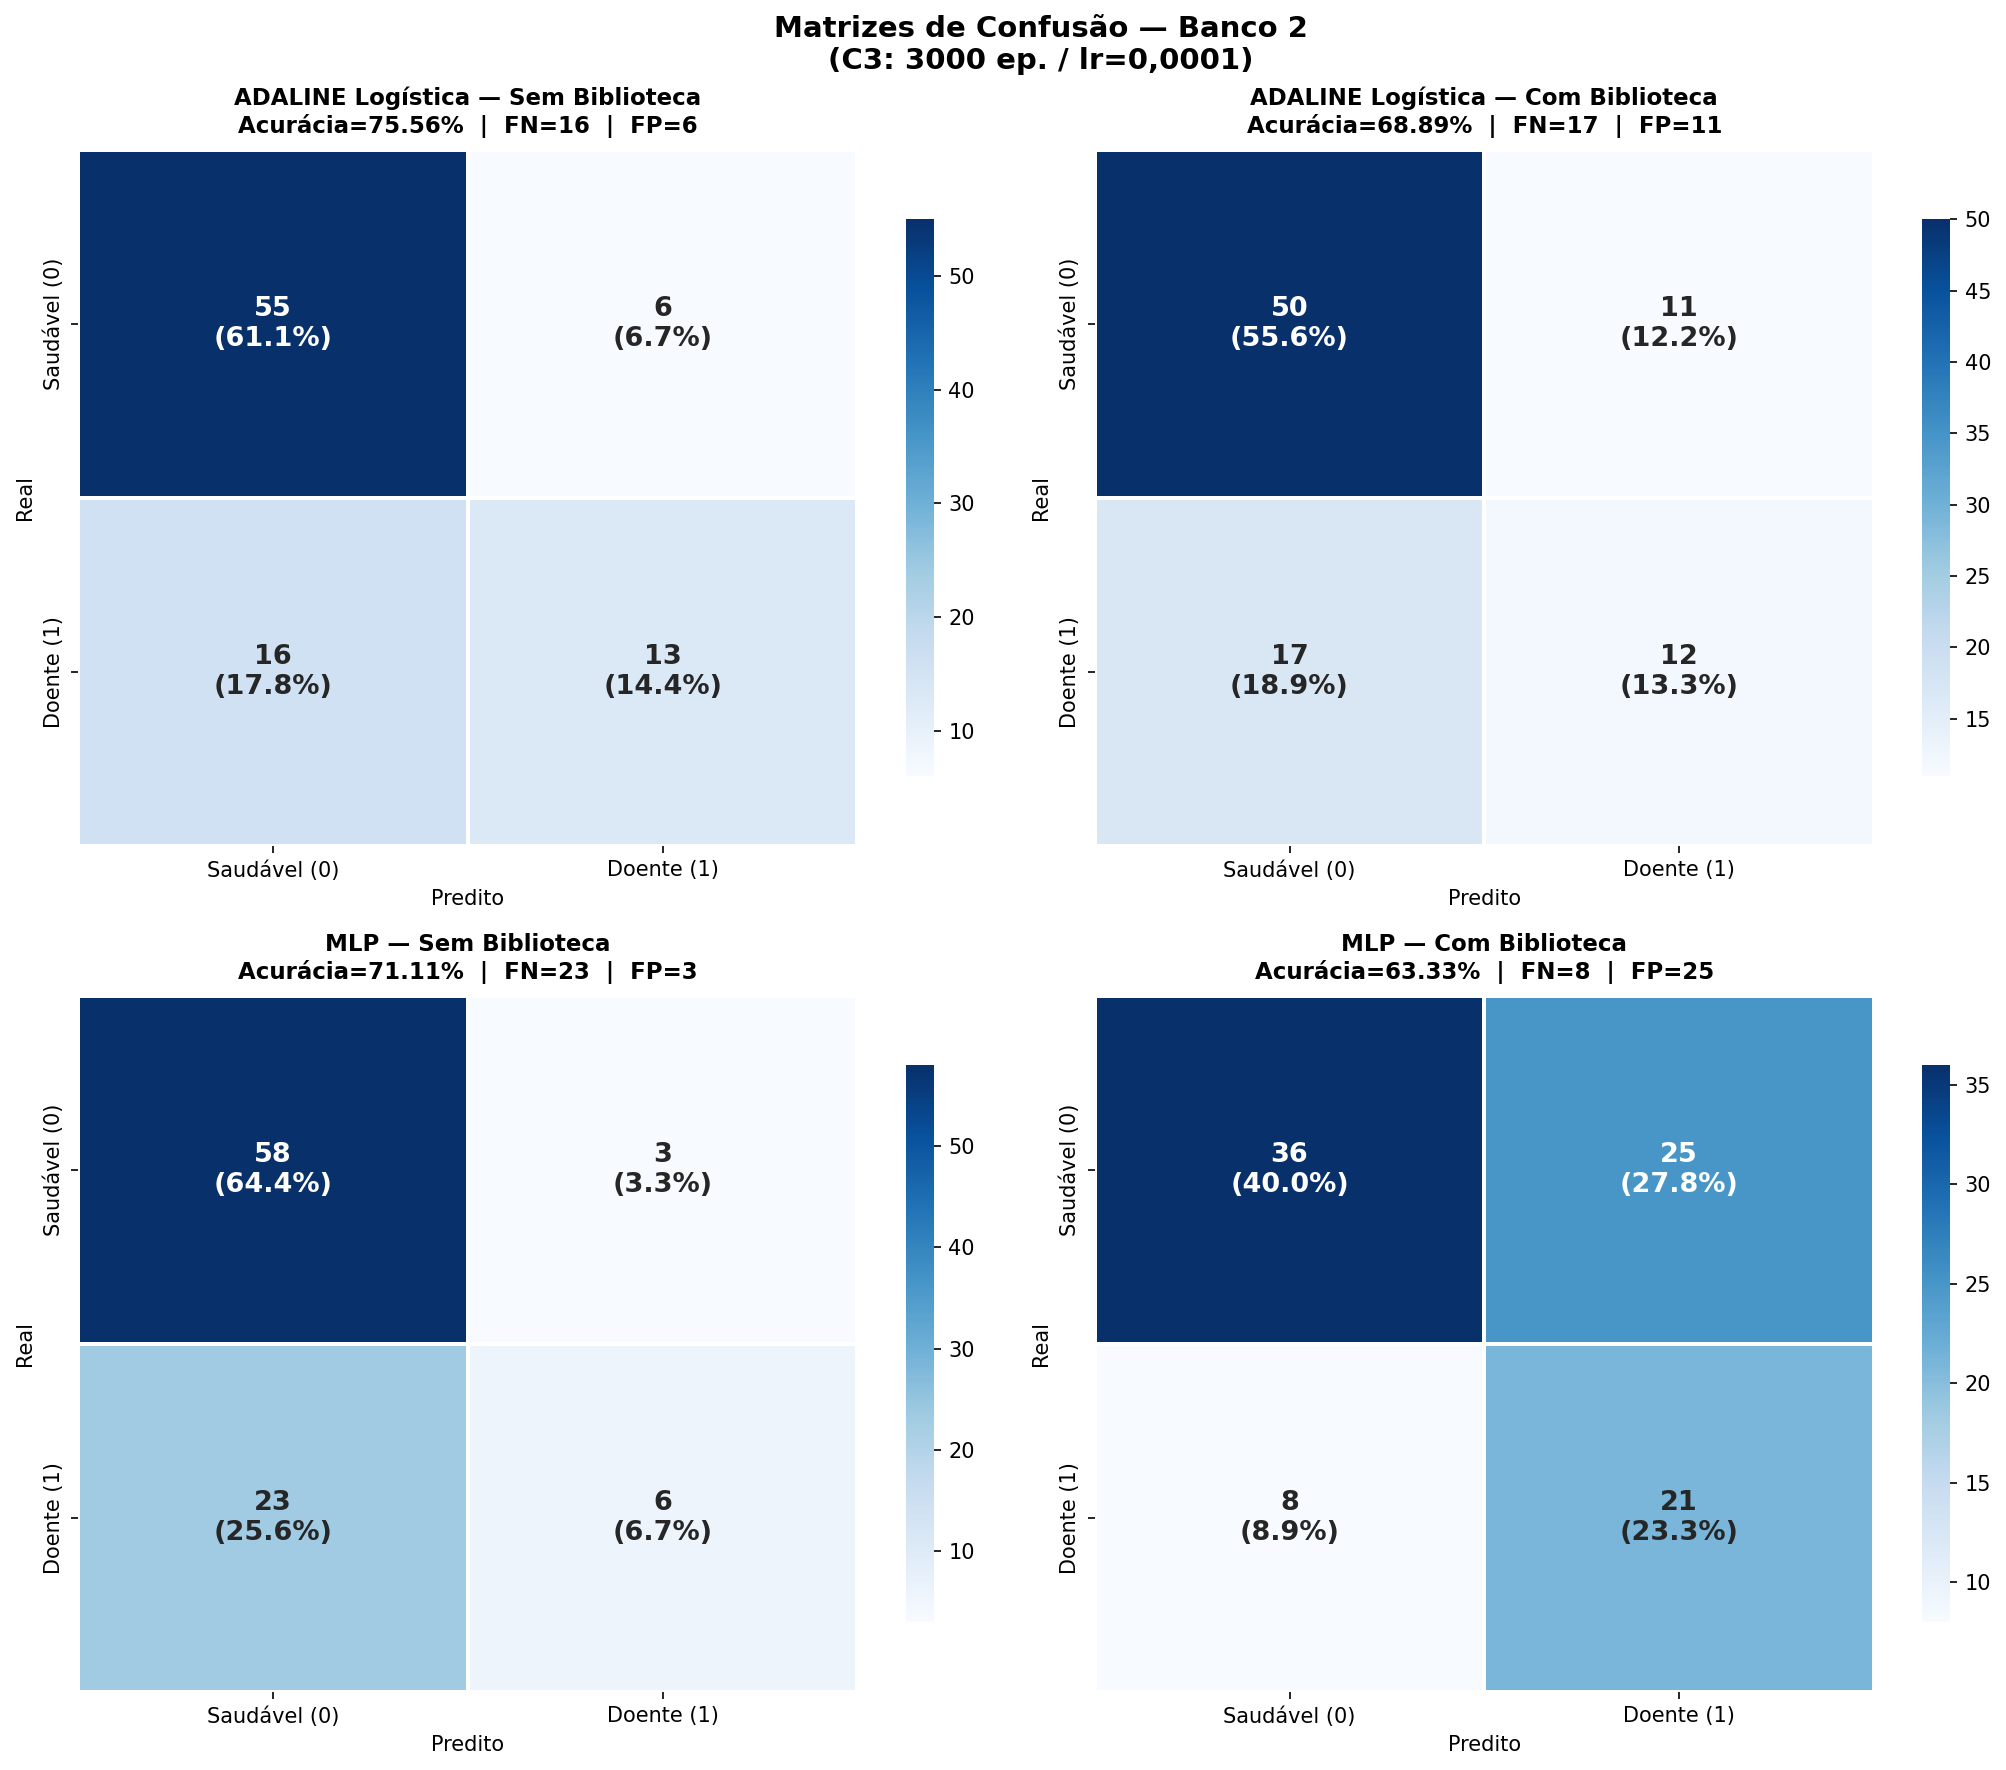
\includegraphics[width=\textwidth]{figuras/resultados/08_matrizes_confusao_banco2.png}
\fonte{Elaborado pelo autor.}
\end{figure}

A Tabela~\ref{tab:metricas_banco2_c3} consolida as métricas de avaliação para C3 calculadas a partir das matrizes de confusão da Figura~\ref{fig:matrizes_banco2}.

\begin{table}[H]
\centering
\caption{Métricas de avaliação dos modelos no Banco 2, configuração C3. Conjunto de teste: 90 pacientes.}
\label{tab:metricas_banco2_c3}
\begin{tabular}{|l|c|c|c|c|c|c|c|}
\hline
\textbf{Modelo} & \textbf{VP} & \textbf{VN} & \textbf{FP} & \textbf{FN} & \textbf{Sensib.} & \textbf{Especif.} & \textbf{Precisão} \\
\hline
ADALINE NumPy   & 13 & 55 & 6  & 16 & 44,83\% & \textbf{90,16\%} & 68,42\% \\
ADALINE Sklearn & 12 & 50 & 11 & 17 & 41,38\% & 81,97\% & 52,17\% \\
MLP NumPy       & 6  & 58 & 3  & 23 & 20,69\% & 95,08\% & 66,67\% \\
MLP Sklearn     & 21 & 36 & 25 & \textbf{8}  & \textbf{72,41\%} & 59,02\% & 45,65\% \\
\hline
\end{tabular}
\fonte{Elaborado pelo autor.}
\end{table}

Os dados da Tabela~\ref{tab:metricas_banco2_c3} expõem a tensão entre sensibilidade e especificidade no Banco 2. O MLP Sklearn em C3 atinge a maior sensibilidade (72,41\%), mas com especificidade de apenas 59,02\%, ou seja, 4 em cada 10 pacientes saudáveis são incorretamente classificados como doentes. O MLP NumPy em C3, por outro lado, atinge especificidade de 95,08\% (quase nenhum falso alarme), mas sensibilidade de apenas 20,69\%, identificando apenas 1 em cada 5 pacientes que vieram a óbito. Esse contraste confirma que, para o Banco 2 em C3, nenhum modelo atingiu simultaneamente sensibilidade e especificidade adequadas para uso clínico, reforçando a superioridade da configuração C1 para o MLP NumPy, que alcançou o melhor equilíbrio entre as duas métricas.

\subsection{Convergência do Erro de Treinamento}
\label{sec:banco2_convergencia}

A Figura~\ref{fig:convergencia_banco2} apresenta a evolução do MSE ao longo das épocas para os quatro modelos no Banco 2, com destaque para o contraste entre a convergência estável dos modelos ADALINE e o comportamento de \textit{overfitting} dos MLPs.

\begin{figure}[H]
\centering
\caption{Convergência do Erro Quadrático Médio (MSE) por época nos quatro modelos, Banco 2.}
\label{fig:convergencia_banco2}
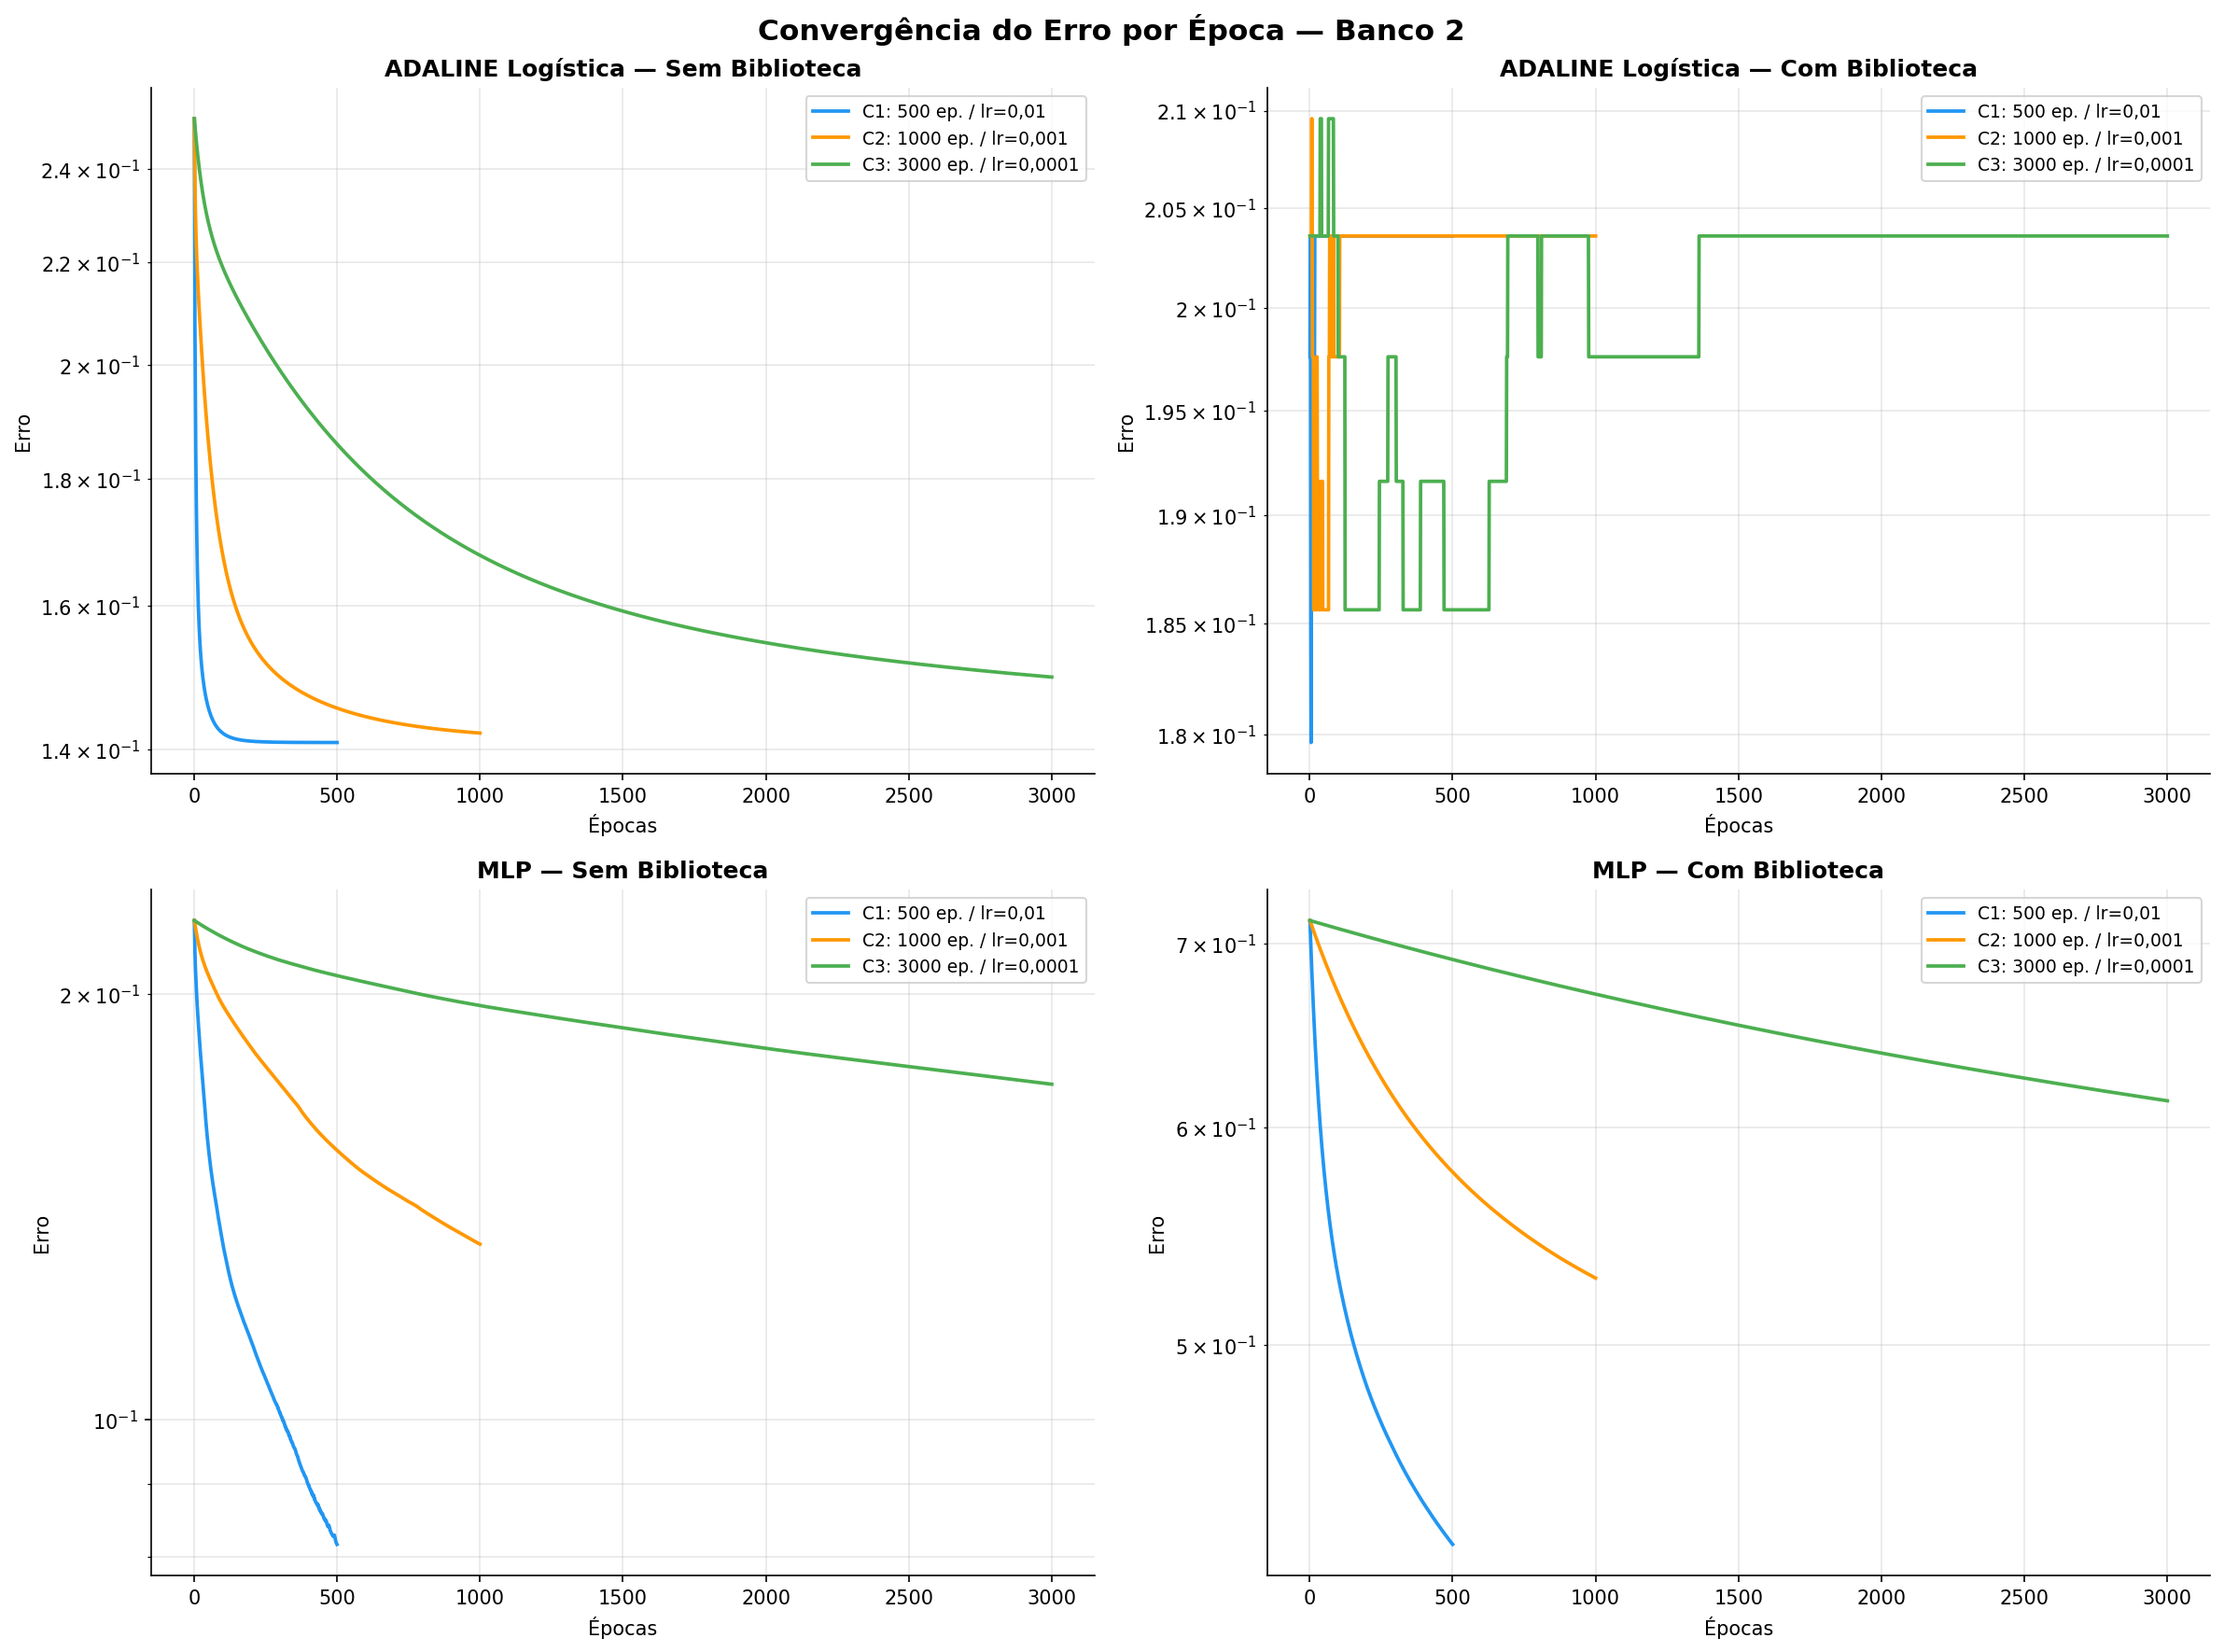
\includegraphics[width=\textwidth]{figuras/resultados/06_convergencia_erro_banco2.png}
\fonte{Elaborado pelo autor.}
\end{figure}

A Figura~\ref{fig:convergencia_banco2} reforça o diagnóstico de \textit{overfitting} nos modelos MLP; os modelos ADALINE convergem de forma suave e estável, coerentemente com seus resultados de acurácia.

Para o MLP NumPy e o MLP Sklearn, o que chama atenção é a velocidade de decrescimento do erro de treino em C1 para ambos: com apenas 500 épocas e taxa $\eta = 0{,}01$, o erro de treinamento cai rapidamente, mais depressa do que nos outros bancos de dados, o que é esperado em conjuntos menores, onde há menos padrões para aprender. Porém, à medida que o número de épocas aumenta (C3), o erro de treino continua decrescendo mesmo quando o desempenho no conjunto de teste piorou, caracterizando o \textit{overfitting}. Esse comportamento é especialmente pronunciado no MLP Sklearn em C3, cujo erro de treinamento é o menor de todos os modelos, mas cuja acurácia de teste é a pior (63,33\%).

\section{Síntese Comparativa entre Modelos e Bancos de Dados}
\label{sec:comparativo}

A visão consolidada dos 24 experimentos é apresentada nas Figuras~\ref{fig:comp_acuracia}, \ref{fig:comp_fn} e \ref{fig:painel_resumo}. A Figura~\ref{fig:comp_acuracia} exibe a acurácia percentual de cada modelo nas três configurações para os dois bancos, permitindo identificar tendências de melhora ou degradação ao longo do treinamento. A Figura~\ref{fig:comp_fn} apresenta o correspondente número de Falsos Negativos, complementando a análise sob o critério clínico prioritário. A Figura~\ref{fig:painel_resumo} resume ambas as métricas exclusivamente para a configuração C3, adotada como referência de comparação final por representar o regime de treinamento mais longo.

\begin{figure}[H]
\centering
\caption{Comparativo de acurácia dos quatro modelos nas três configurações, para os dois bancos de dados.}
\label{fig:comp_acuracia}
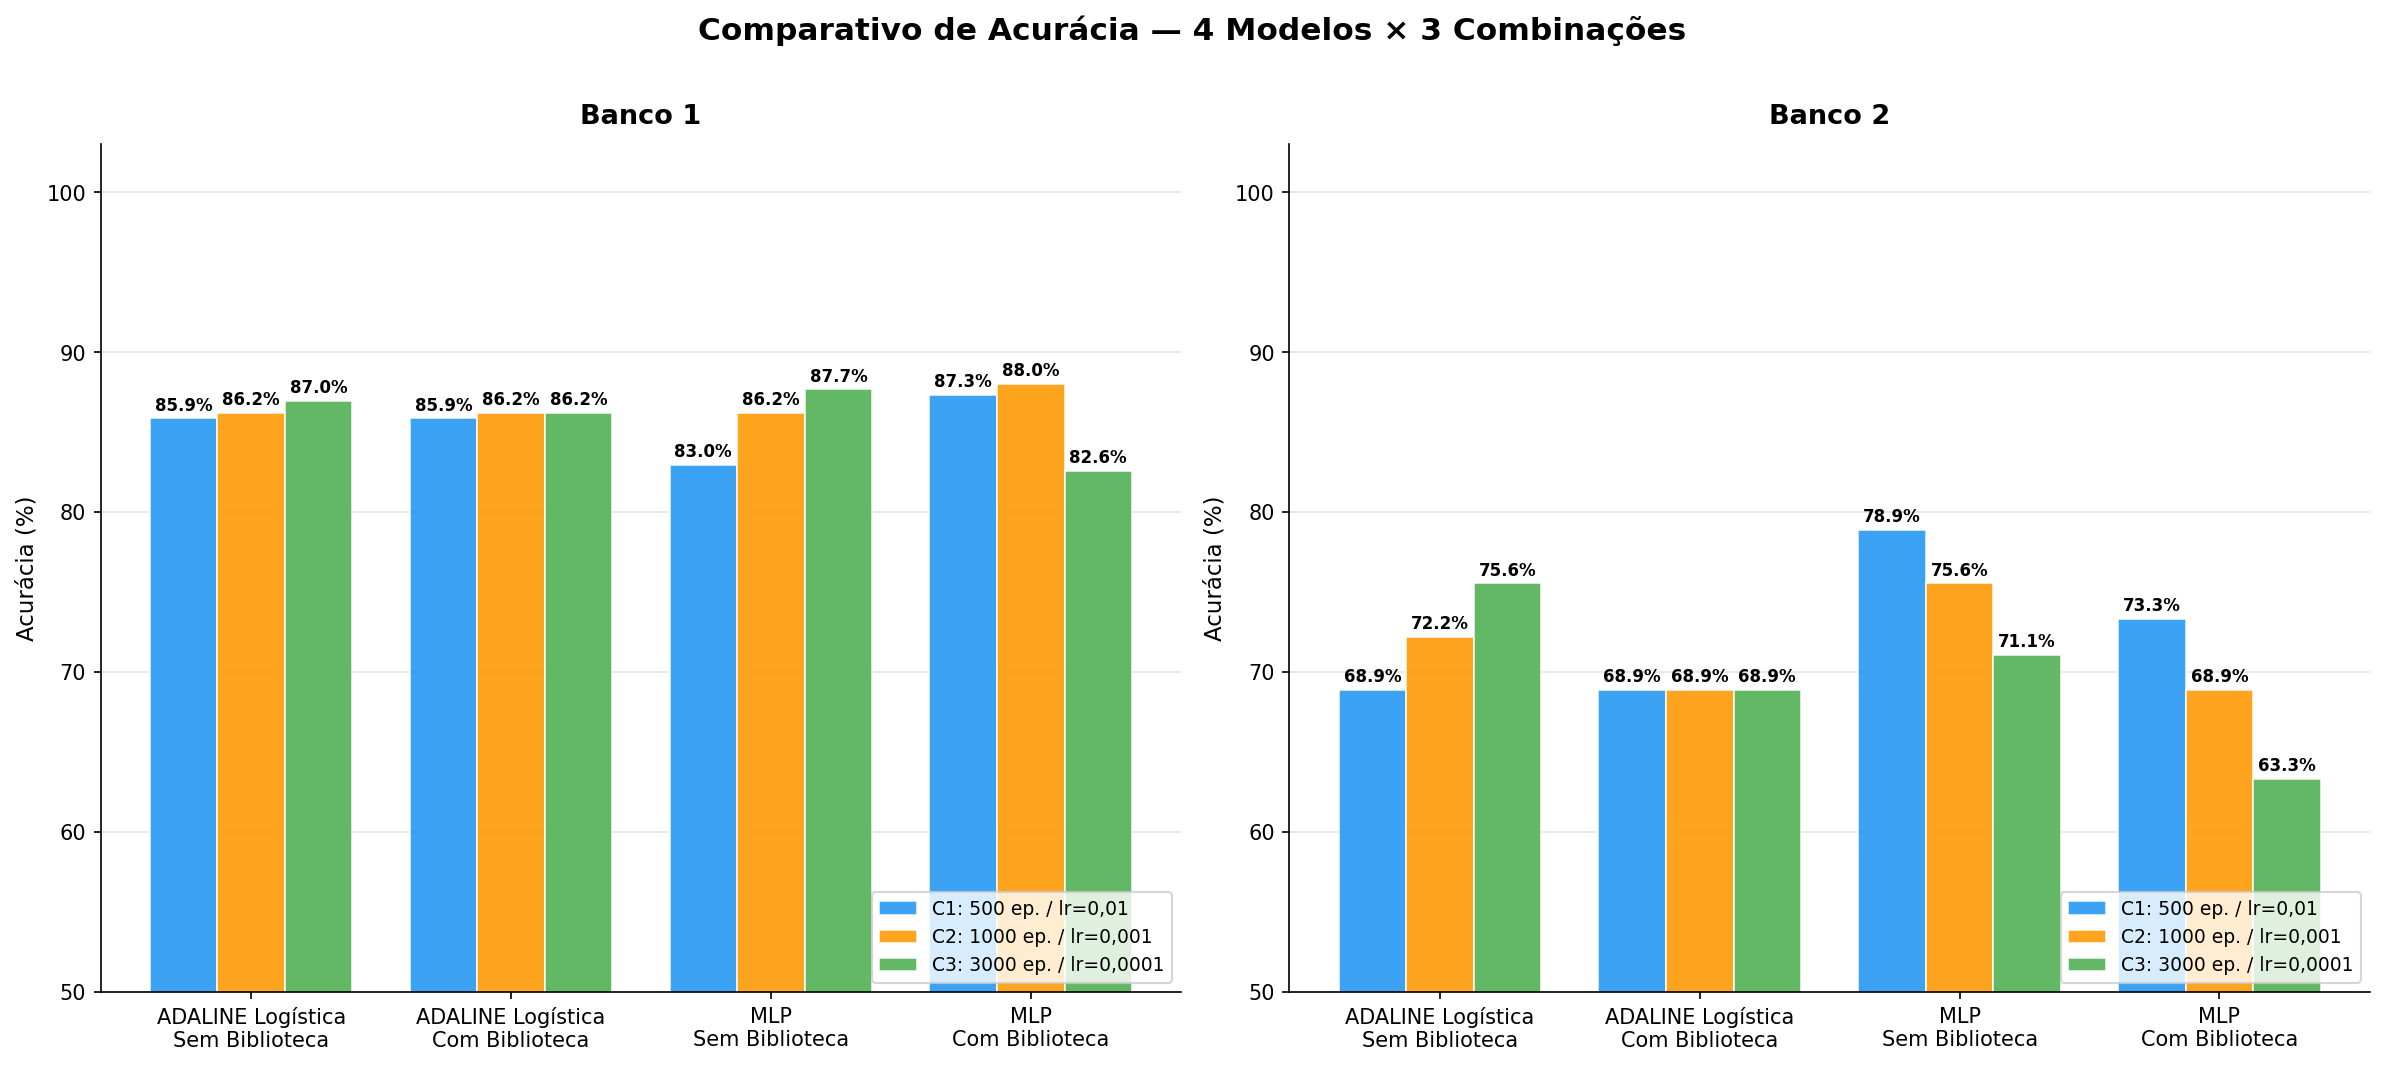
\includegraphics[width=\textwidth]{figuras/resultados/01_comparativo_acuracia.png}
\fonte{Elaborado pelo autor.}
\end{figure}

\begin{figure}[H]
\centering
\caption{Comparativo de Falsos Negativos dos quatro modelos nas três configurações, para os dois bancos de dados.}
\label{fig:comp_fn}
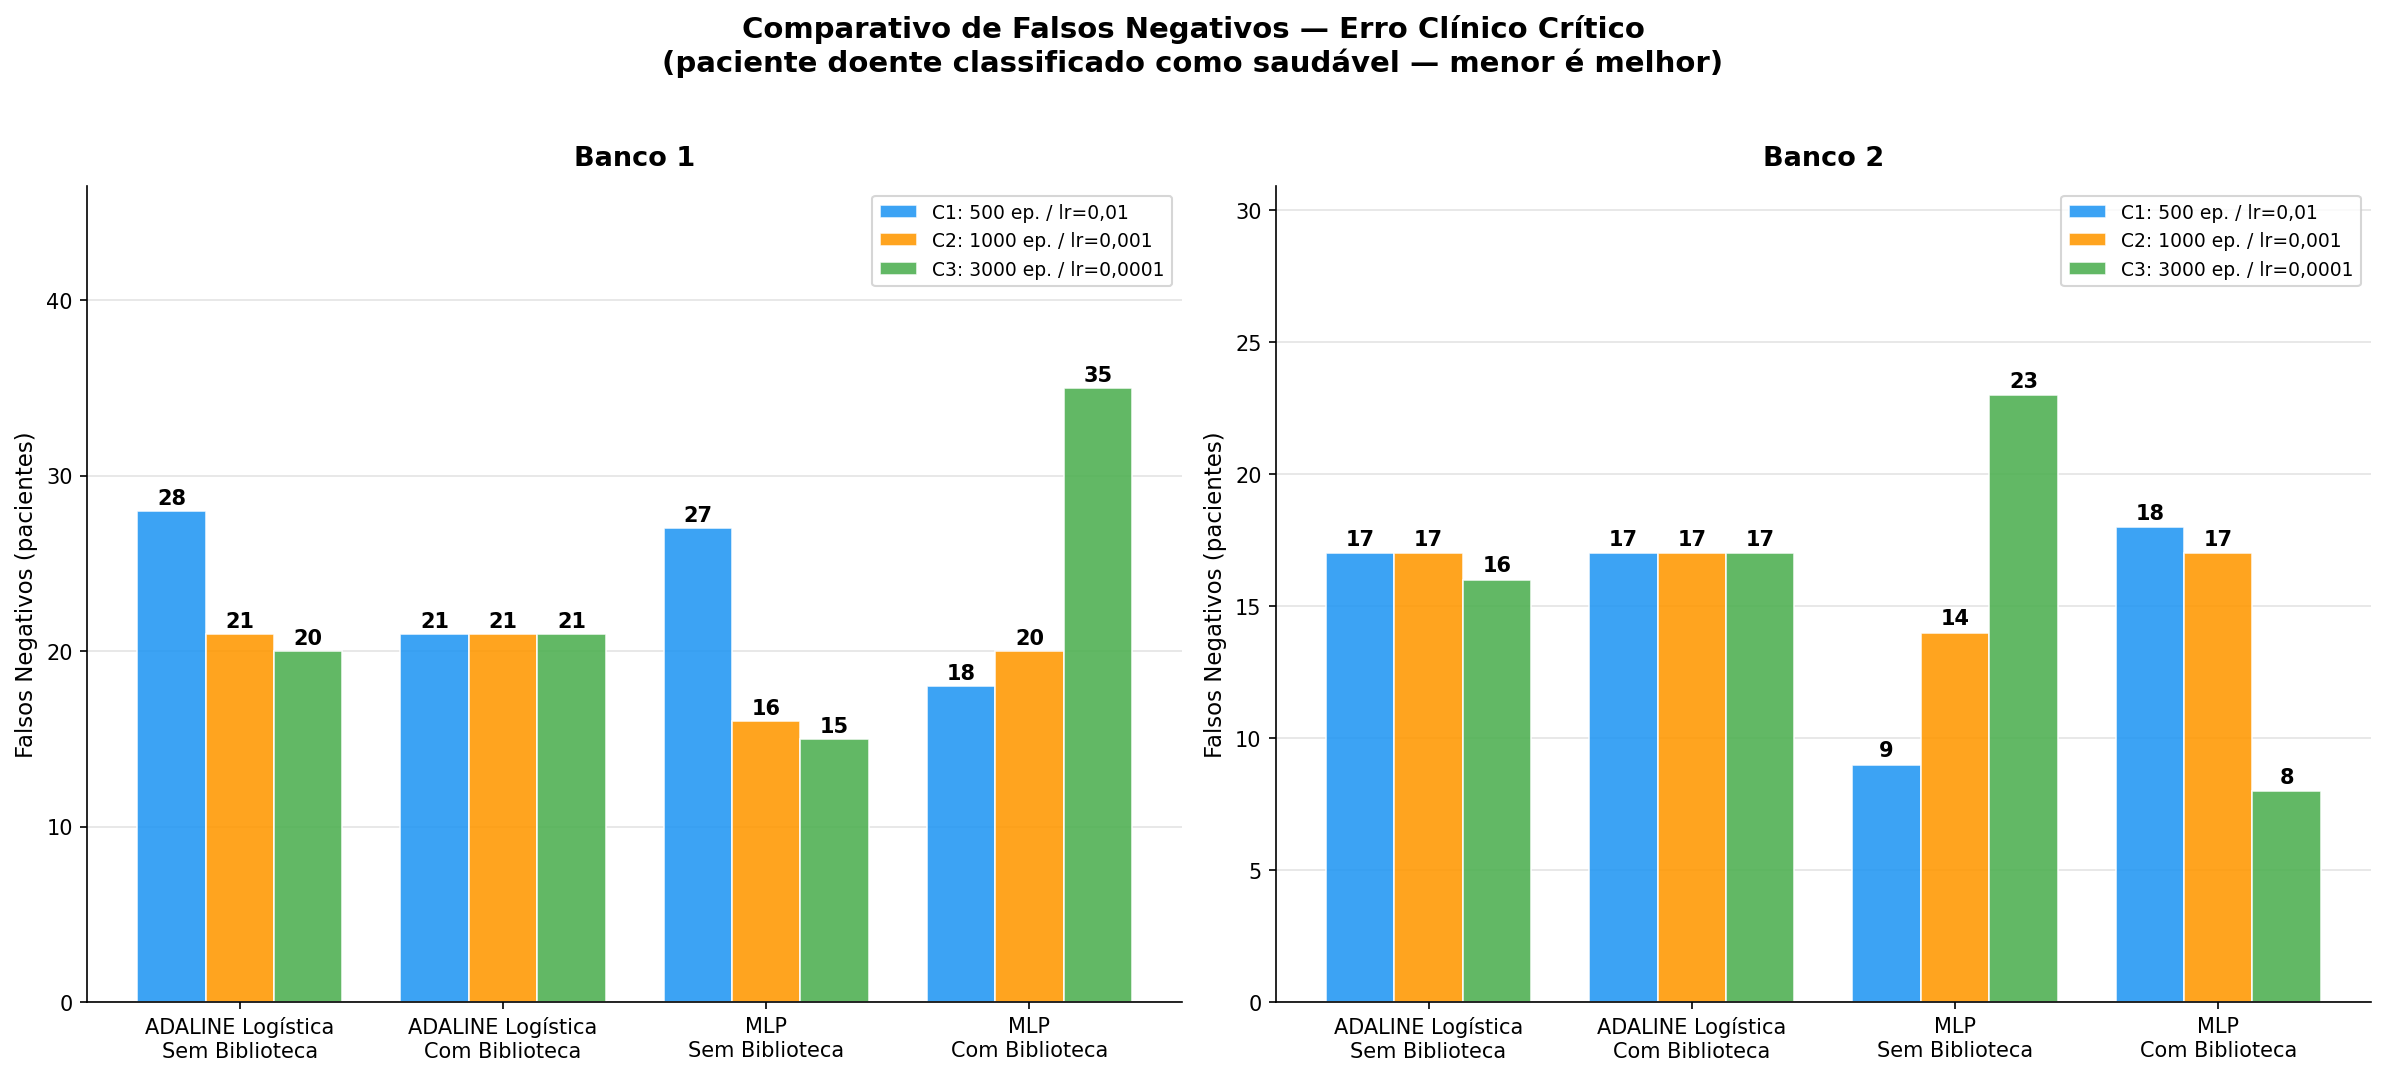
\includegraphics[width=\textwidth]{figuras/resultados/02_comparativo_falsos_negativos.png}
\fonte{Elaborado pelo autor.}
\end{figure}

\begin{figure}[H]
\centering
\caption{Painel resumo comparativo da configuração C3 (3.000 épocas, $\eta$ = 0,0001) para os dois bancos de dados: acurácia (superior) e Falsos Negativos (inferior).}
\label{fig:painel_resumo}
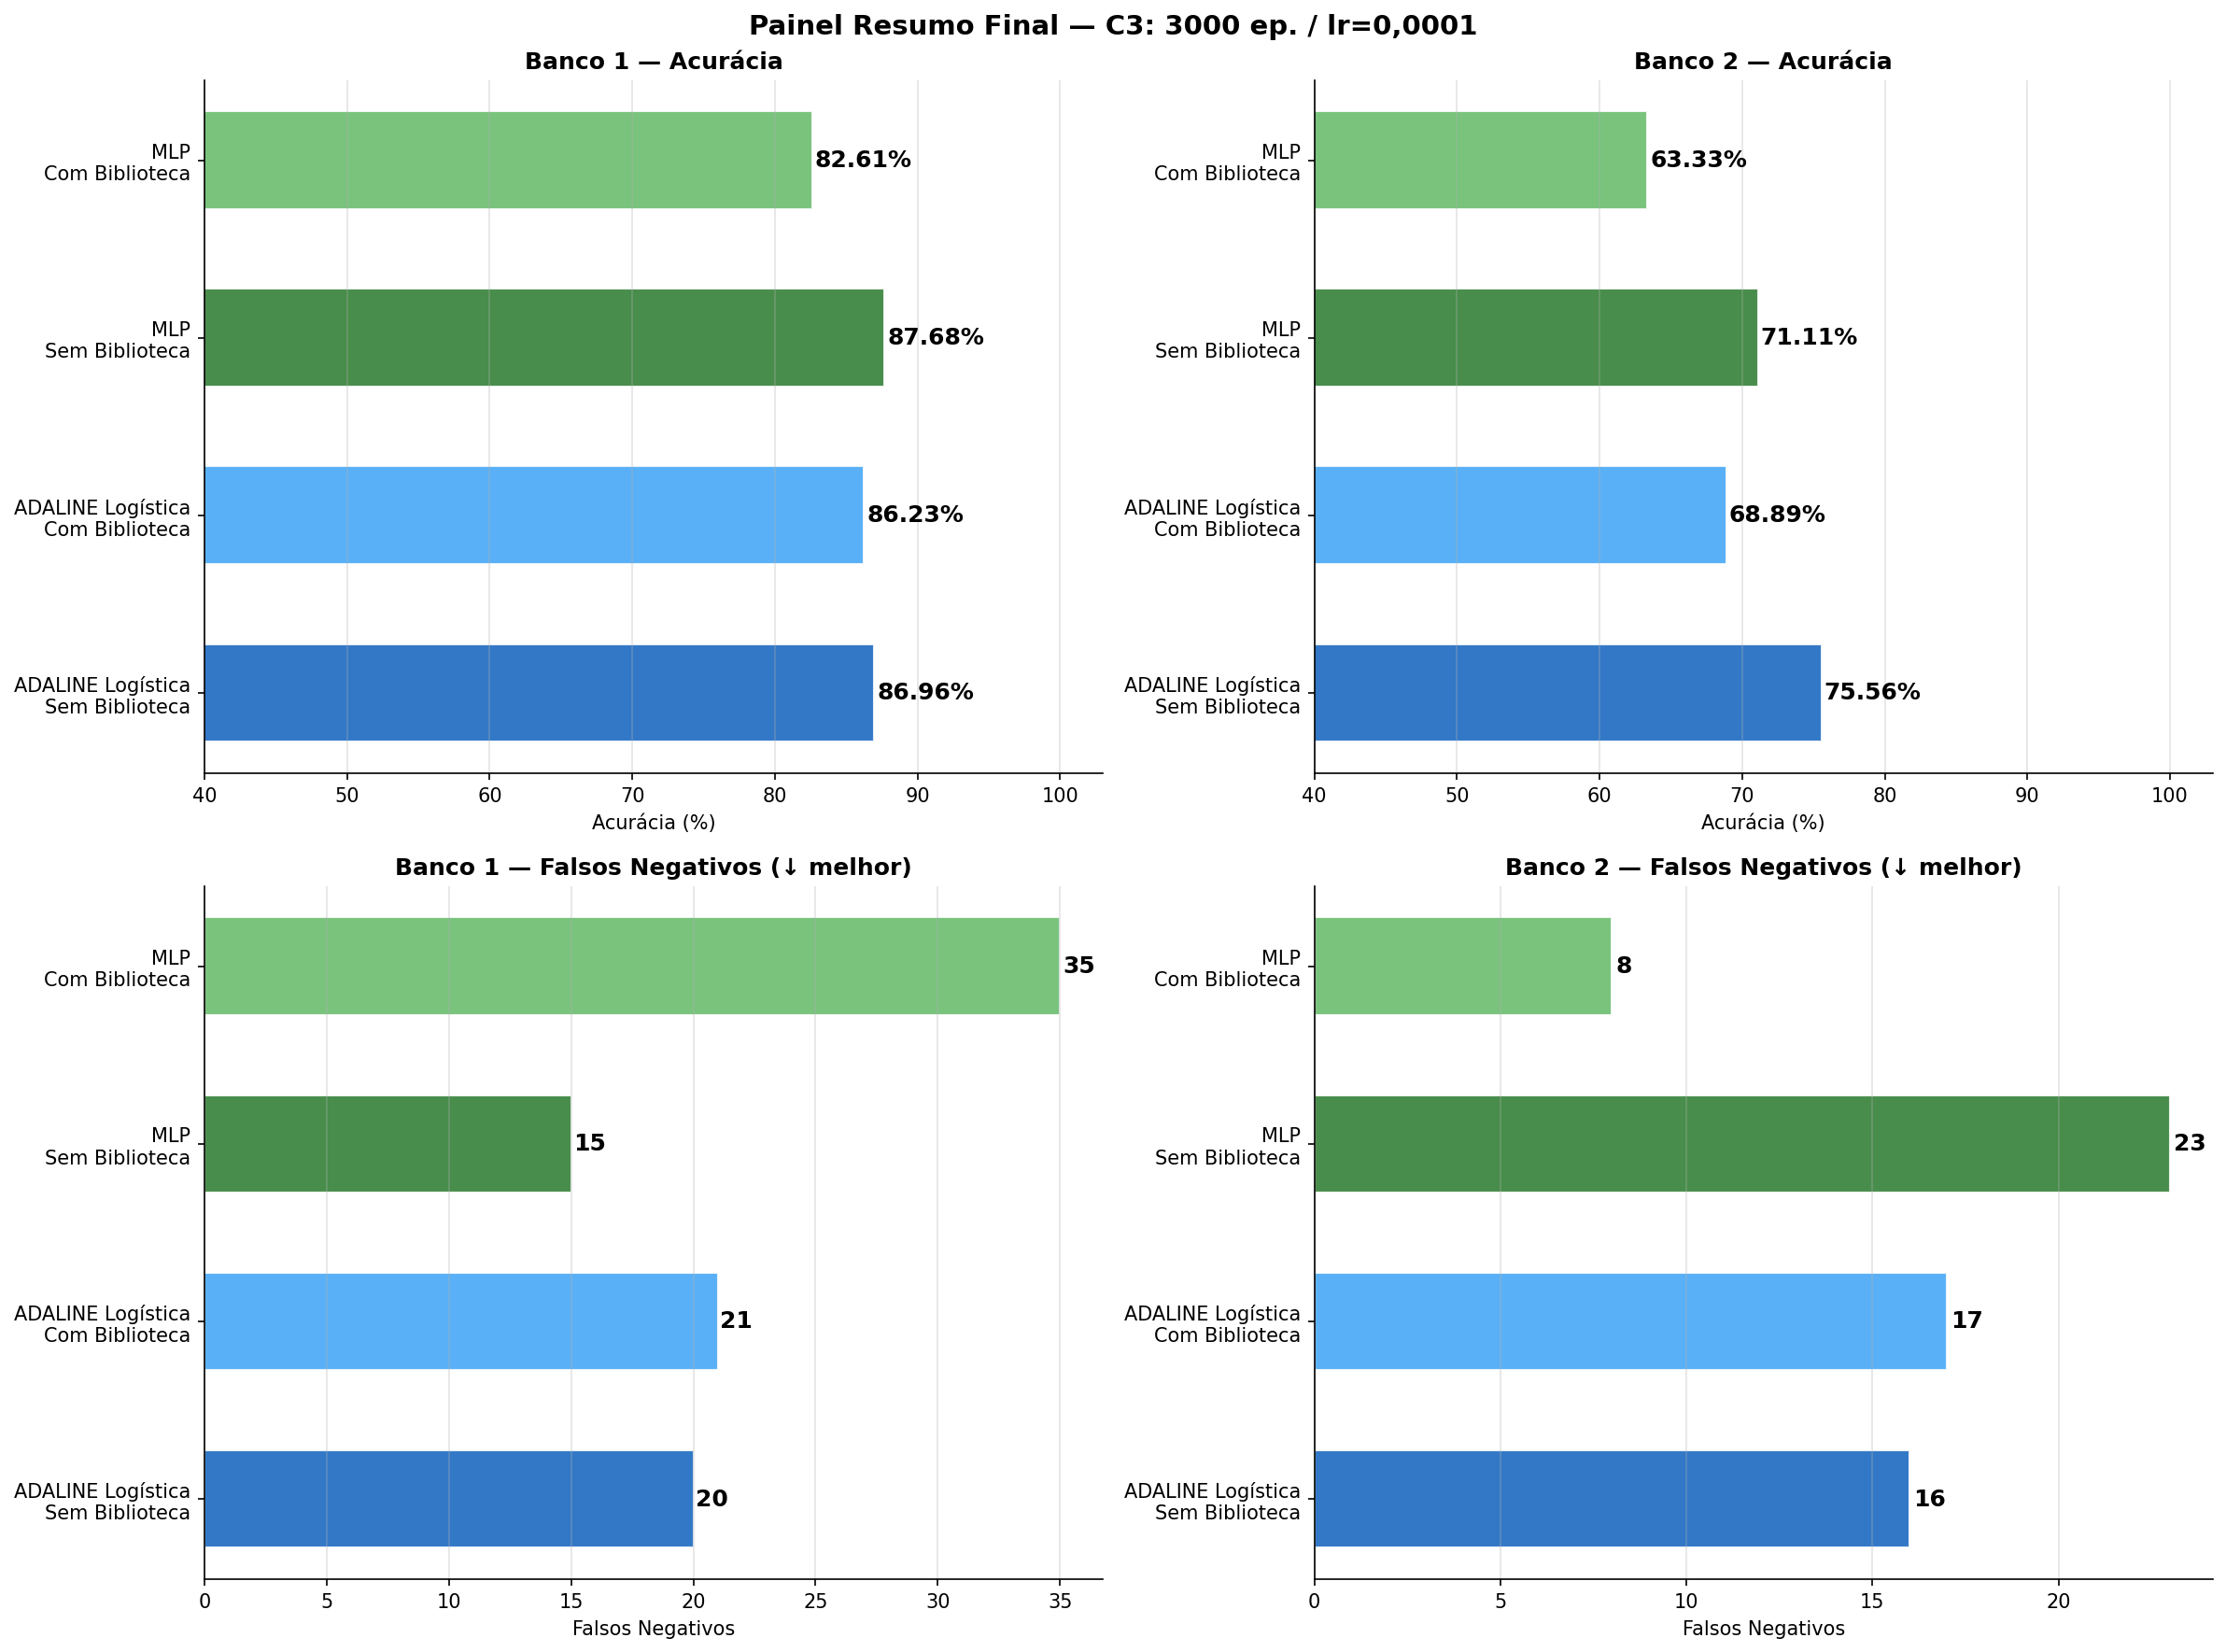
\includegraphics[width=\textwidth]{figuras/resultados/09_painel_resumo_final.png}
\fonte{Elaborado pelo autor.}
\end{figure}

A Tabela~\ref{tab:resumo_geral} sintetiza os melhores resultados por critério e banco de dados.

\begin{table}[H]
\centering
\caption{Síntese dos melhores resultados por critério e banco de dados.}
\label{tab:resumo_geral}
\begin{tabular}{|l|l|c|c|}
\hline
\textbf{Banco} & \textbf{Critério} & \textbf{Melhor modelo / config.} & \textbf{Valor} \\
\hline
Banco 1 & Maior acurácia         & MLP Sklearn C2        & 88,04\% \\
Banco 1 & Menor FN (clínico)     & MLP NumPy C3          & 15 FNs (Sens. 90,20\%) \\
Banco 2 & Maior acurácia         & MLP NumPy C1          & 78,89\% \\
Banco 2 & Menor FN (clínico)     & MLP Sklearn C3        & 8 FNs (Sens. 72,41\%) \\
Banco 2 & Melhor equilíbrio      & MLP NumPy C1          & 78,89\% / 9 FNs \\
\hline
\end{tabular}
\fonte{Elaborado pelo autor.}
\end{table}

\subsection{Considerações Finais sobre os Resultados}
\label{sec:consideracoes_resultados}

\begin{itemize}
    \item No Banco 1, o MLP NumPy em C3 é o modelo recomendado sob o critério clínico de minimização de Falsos Negativos: 87,68\% de acurácia e 15 FNs, com sensibilidade de 90,20\%. O MLP Sklearn em C2 é o melhor em acurácia absoluta (88,04\%), mas com maior FN (20).

    \item No Banco 2, o MLP NumPy em C1 oferece o melhor equilíbrio geral: 78,89\% de acurácia e 9 FNs, com sensibilidade de 68,97\%. Configurações mais longas causam \textit{overfitting} evidente neste modelo.

    \item O ADALINE NumPy mostrou comportamento consistente e previsível nos dois bancos, com melhora gradual e sem degradação em nenhuma configuração. Sua estabilidade o torna adequado em cenários onde a confiabilidade do comportamento é prioridade.

    \item O ADALINE Sklearn apresentou rigidez de comportamento com FNs idênticos em todas as configurações do Banco 2 e acurácia estacionária, limitando sua utilidade em cenários que exigem ajuste fino.

    \item A superioridade esperada do MLP sobre o ADALINE não se materializou de forma consistente, em razão do volume limitado de dados e da instabilidade do SGD com momento em datasets pequenos com muitas épocas, fatores confirmados empiricamente pelo experimento complementar da Seção~\ref{sec:resultados_bruto}, que descartou a binarização como fator determinante.
\end{itemize}

\section{Experimento Complementar: Dados Originais sem Binarização}
\label{sec:resultados_bruto}

Para verificar o efeito da binarização sobre o desempenho relativo dos modelos, os quatro algoritmos foram reaplicados sobre os dados brutos, substituindo a binarização clínica por \textit{one-hot encoding} para as variáveis categóricas do Banco~1 e padronização \textit{z-score} (\texttt{StandardScaler}) para as variáveis numéricas. O Banco~1 resultou em 18 características (contra 35 do experimento binarizado) e o Banco~2 em 12 (contra 14). A divisão treino/validação/teste e as três configurações foram mantidas idênticas ao experimento principal.

\subsection{Resultados no Banco 1 com Dados Brutos}
\label{sec:bruto_banco1}

A Tabela~\ref{tab:bruto_banco1} apresenta a acurácia e o número de Falsos Negativos obtidos pelos quatro modelos nas três configurações, com dados brutos do Banco~1.

\begin{table}[H]
\centering
\caption{Acurácia (\%) e Falsos Negativos (FN), Banco 1, dados brutos. Conjunto de teste: 276 pacientes.}
\label{tab:bruto_banco1}
\resizebox{\textwidth}{!}{%
\begin{tabular}{|l|c|c|c|c|c|c|}
\hline
\multirow{2}{*}{\textbf{Modelo}} & \multicolumn{2}{c|}{\textbf{C1 (500 ep. / $\eta$=0,01)}} & \multicolumn{2}{c|}{\textbf{C2 (1000 ep. / $\eta$=0,001)}} & \multicolumn{2}{c|}{\textbf{C3 (3000 ep. / $\eta$=0,0001)}} \\
\cline{2-7}
 & \textbf{Acurácia} & \textbf{FN} & \textbf{Acurácia} & \textbf{FN} & \textbf{Acurácia} & \textbf{FN} \\
\hline
ADALINE NumPy   & 87,68\% & 16 & 87,68\% & 16 & 87,68\% & 16 \\
ADALINE Sklearn & 88,04\% & 15 & 87,32\% & 16 & 87,68\% & 16 \\
MLP NumPy       & 86,96\% & 16 & 87,32\% & 17 & \textbf{88,77\%} & \textbf{14} \\
MLP Sklearn     & 86,59\% & 14 & 86,59\% & 16 & 81,52\% & 22 \\
\hline
\end{tabular}}
\fonte{Elaborado pelo autor.}
\end{table}

No Banco~1, o ADALINE NumPy convergiu para 87,68\% em todas as configurações (superior ao melhor binarizado, 86,96\%), e o MLP NumPy atingiu 88,77\% / 14~FNs em C3, superando seu melhor resultado binarizado (87,68\% / 15~FNs). O MLP Sklearn manteve a instabilidade em C3 (81,52\%, 22~FNs), replicando o padrão do experimento principal.

\subsection{Resultados no Banco 2 com Dados Brutos}
\label{sec:bruto_banco2}

A Tabela~\ref{tab:bruto_banco2} apresenta os resultados do Banco~2 com dados brutos.

\begin{table}[H]
\centering
\caption{Acurácia (\%) e Falsos Negativos (FN), Banco 2, dados brutos. Conjunto de teste: 90 pacientes (29 óbitos / 61 sobreviventes).}
\label{tab:bruto_banco2}
\resizebox{\textwidth}{!}{%
\begin{tabular}{|l|c|c|c|c|c|c|}
\hline
\multirow{2}{*}{\textbf{Modelo}} & \multicolumn{2}{c|}{\textbf{C1 (500 ep. / $\eta$=0,01)}} & \multicolumn{2}{c|}{\textbf{C2 (1000 ep. / $\eta$=0,001)}} & \multicolumn{2}{c|}{\textbf{C3 (3000 ep. / $\eta$=0,0001)}} \\
\cline{2-7}
 & \textbf{Acurácia} & \textbf{FN} & \textbf{Acurácia} & \textbf{FN} & \textbf{Acurácia} & \textbf{FN} \\
\hline
ADALINE NumPy   & \textbf{82,22\%} & \textbf{11} & \textbf{82,22\%} & \textbf{11} & \textbf{82,22\%} & \textbf{11} \\
ADALINE Sklearn & 83,33\% & 11 & 83,33\% & 11 & 82,22\% & 11 \\
MLP NumPy       & 80,00\% & 12 & 81,11\% & 12 & 78,89\% & 14 \\
MLP Sklearn     & 81,11\% & 11 & 66,67\% & 15 & 45,56\% & 10 \\
\hline
\end{tabular}}
\fonte{Elaborado pelo autor.}
\end{table}

No Banco~2, os dados brutos trouxeram ganhos expressivos para os ADALINEs: o ADALINE NumPy atingiu 82,22\% / 11~FNs em todas as configurações e o ADALINE Sklearn 83,33\% em C1 e C2, contra a faixa de 68,89\%--75,56\% do experimento binarizado. O ganho de até 14 pontos percentuais demonstra que os biomarcadores contínuos do Banco~2 carregam informação prognóstica que a discretização por limiar clínico não captura. Os MLPs não se beneficiaram dos dados brutos: o MLP NumPy degradou-se de 80,00\% (C1) para 78,89\% (C3), e o MLP Sklearn colapsou para 45,56\% em C3, o pior resultado de todos os 24 experimentos realizados.

\subsection{Comparação: Binarizado versus Bruto}
\label{sec:comparativo_binarizado_bruto}

A Figura~\ref{fig:comparativo_binarizado_vs_bruto} apresenta a comparação direta dos resultados binarizados e brutos na configuração C3 para os dois bancos, em termos de acurácia e Falsos Negativos. As Figuras~\ref{fig:acuracia_bruto} e \ref{fig:fn_bruto} complementam essa análise exibindo, respectivamente, a acurácia e os Falsos Negativos nas três configurações de treinamento com dados brutos.

\begin{figure}[H]
\centering
\caption[Comparativo binarizado vs.\ bruto, configuração C3.]{Comparativo entre o experimento principal (dados binarizados) e o experimento complementar (dados brutos + StandardScaler) na configuração C3, para os dois bancos de dados. Painel superior: acurácia (\%); painel inferior: Falsos Negativos.}
\label{fig:comparativo_binarizado_vs_bruto}
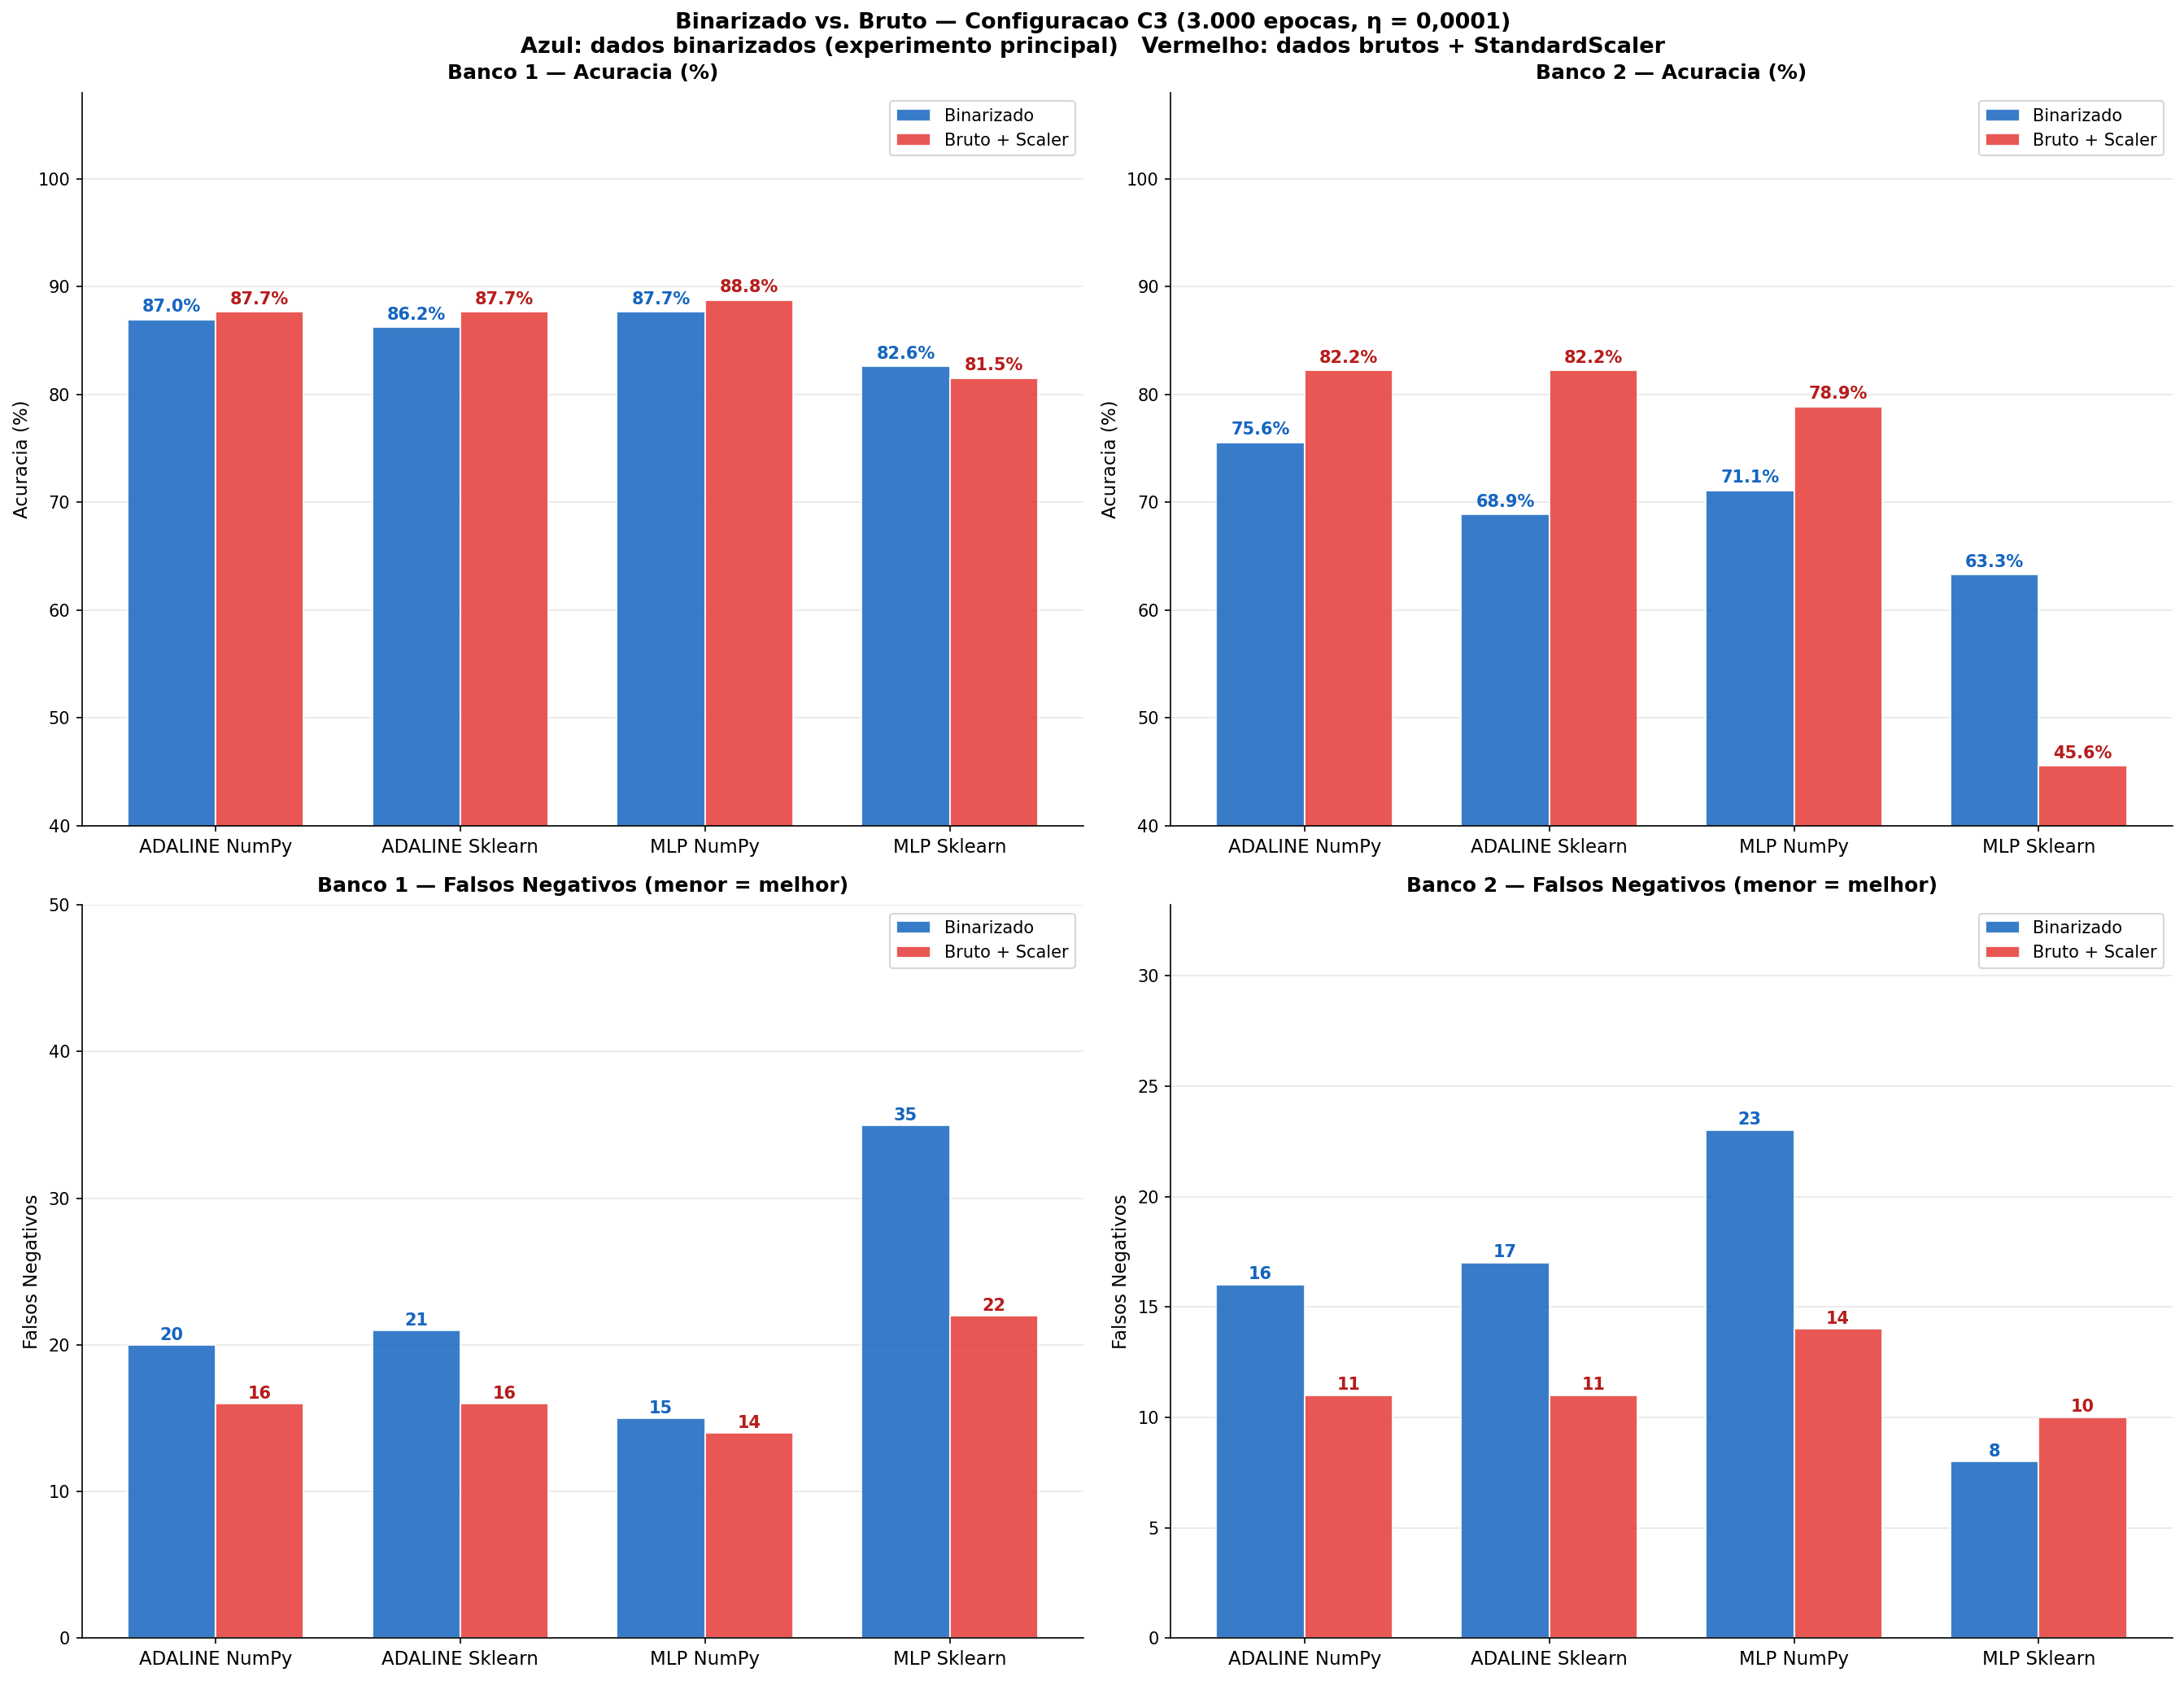
\includegraphics[width=\textwidth]{figuras/resultados/10_comparativo_binarizado_vs_bruto.png}
\fonte{Elaborado pelo autor.}
\end{figure}

\begin{figure}[H]
\centering
\caption{Acurácia dos quatro modelos nas três configurações de treinamento, com dados brutos e StandardScaler.}
\label{fig:acuracia_bruto}
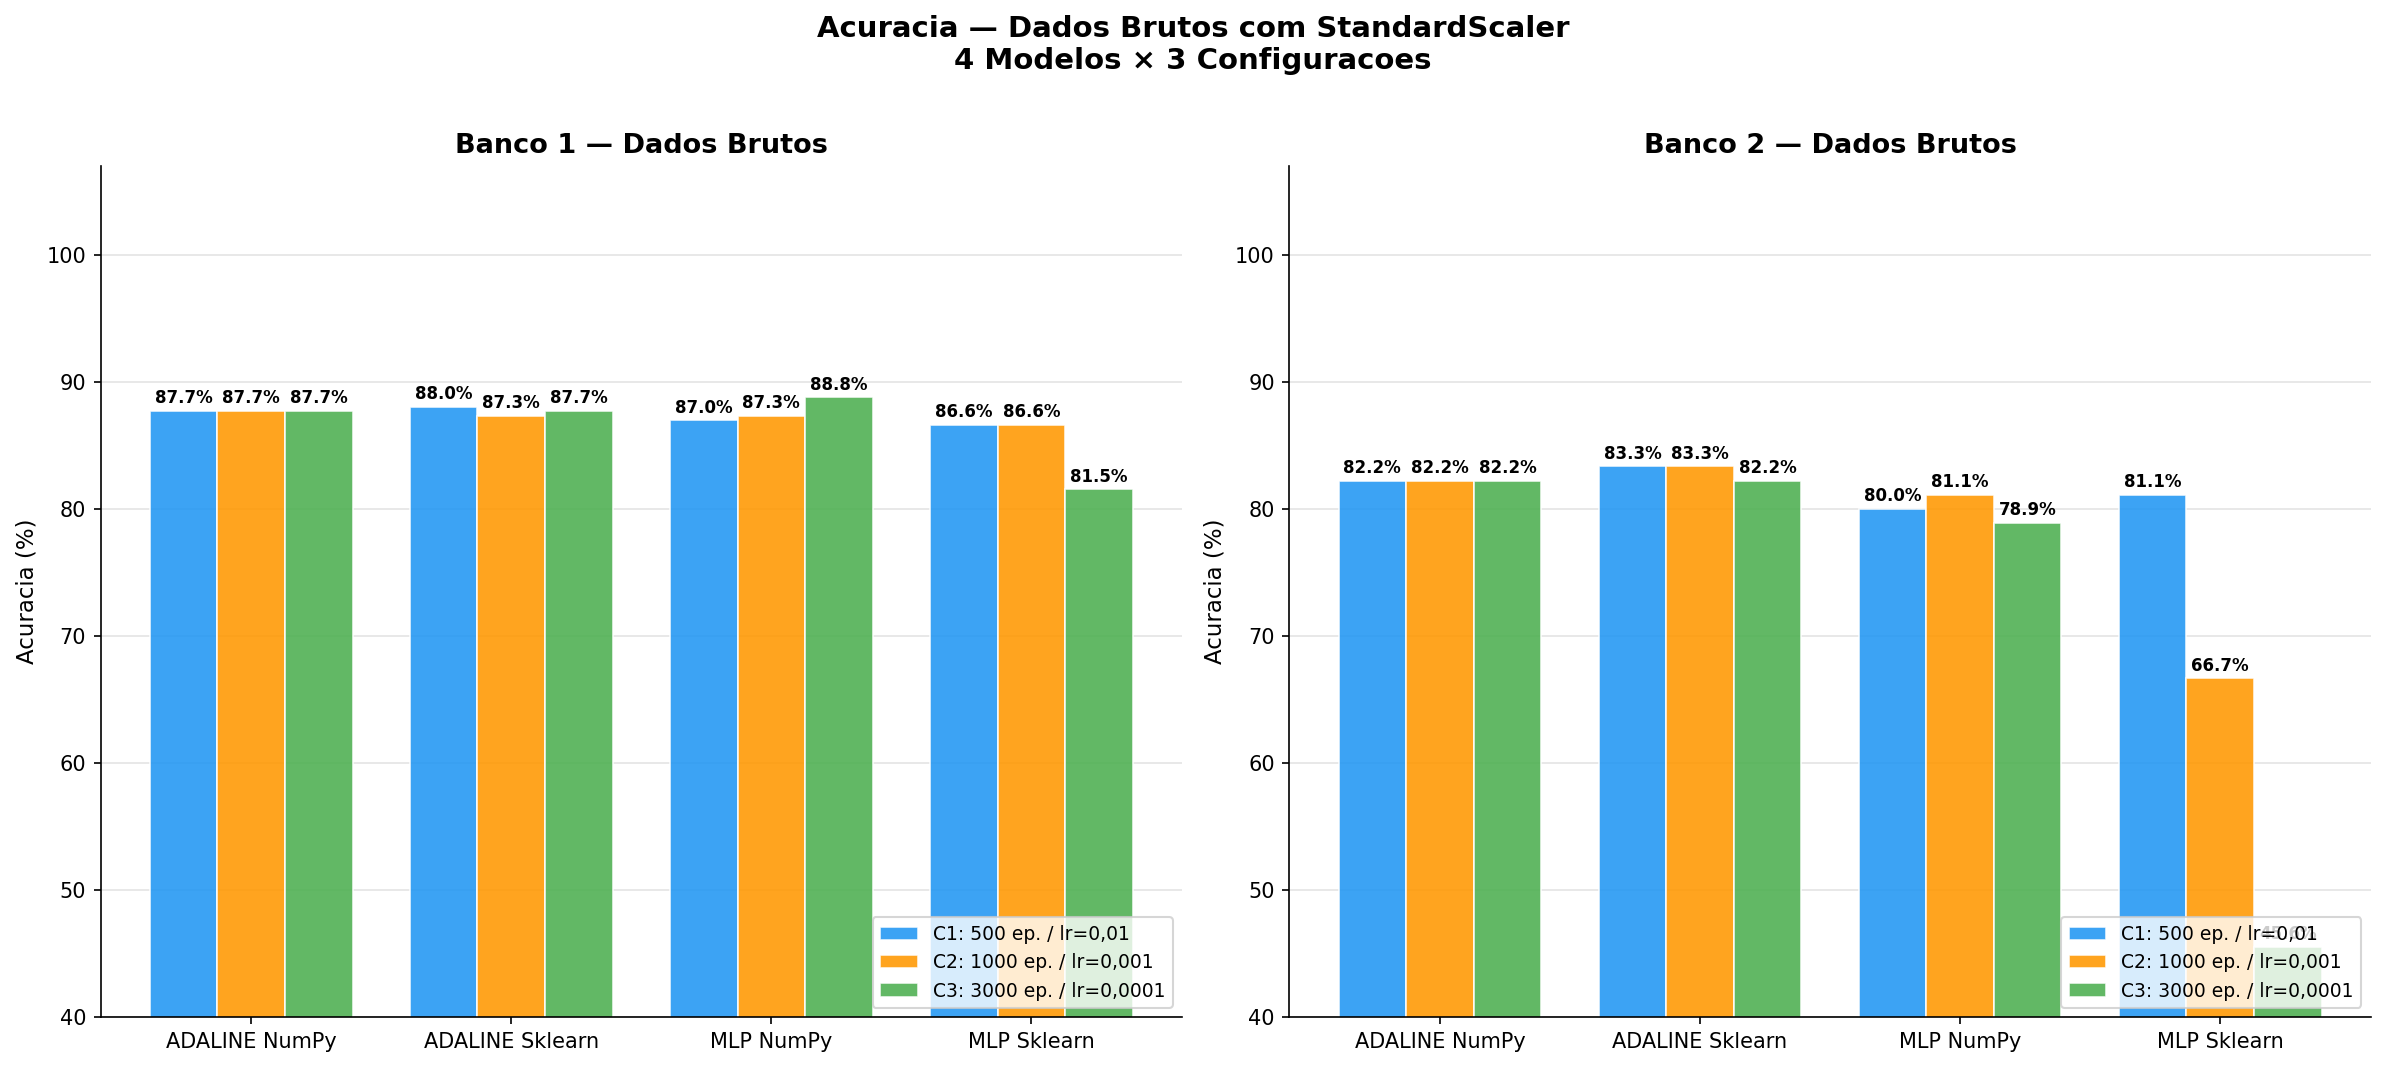
\includegraphics[width=\textwidth]{figuras/resultados/11_acuracia_bruto.png}
\fonte{Elaborado pelo autor.}
\end{figure}

\begin{figure}[H]
\centering
\caption{Falsos Negativos dos quatro modelos nas três configurações de treinamento, com dados brutos e StandardScaler.}
\label{fig:fn_bruto}
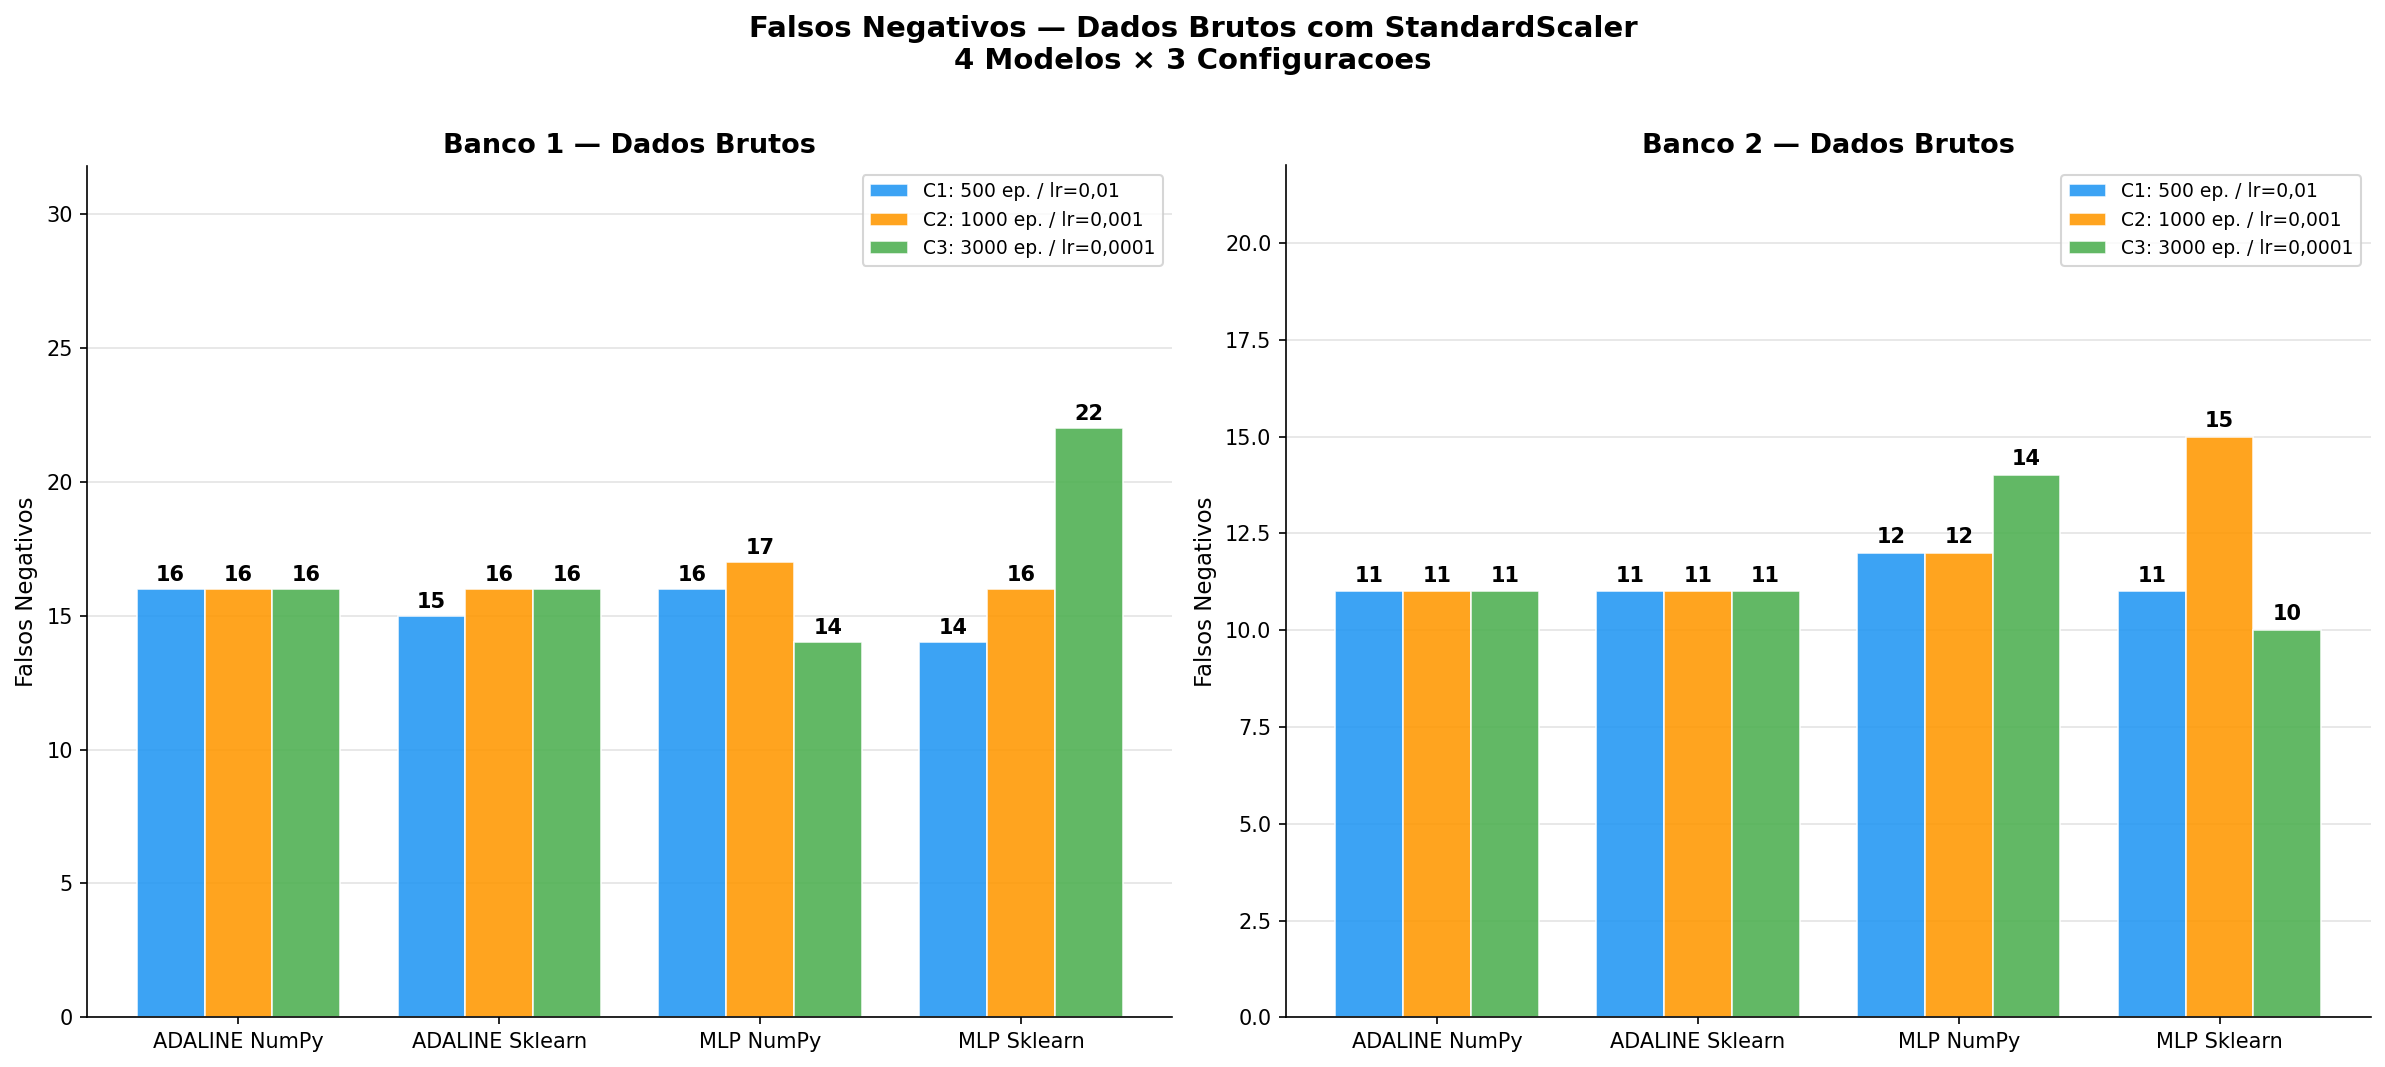
\includegraphics[width=\textwidth]{figuras/resultados/12_fn_bruto.png}
\fonte{Elaborado pelo autor.}
\end{figure}

A conclusão deste experimento é que a binarização não foi a principal responsável pela competitividade do ADALINE: mesmo com dados contínuos, os ADALINEs se mostraram mais estáveis e, no Banco~2, mais acurados do que os MLPs. O fator determinante é o volume de dados disponível para o treinamento, que favorece sistematicamente o modelo mais simples. A persistência da vantagem do ADALINE com representação contínua é consistente com a hipótese de que a fronteira de decisão nesses dados é predominantemente linear, embora o volume reduzido de treinamento impeça confirmar categoricamente essa interpretação. Essa questão é retomada na Seção~\ref{sec:discussao_mlp}.

\chapter{Discuss\~ao}
\label{cap:discussao}

Este cap\'itulo interpreta os resultados apresentados no Cap\'itulo~\ref{cap:resultados} \`a luz dos fundamentos te\'oricos do Cap\'itulo~\ref{cap:fundamentacao} e dos estudos relacionados do Cap\'itulo~\ref{cap:trabalhos}, respondendo \`a quest\~ao central do trabalho e situando as constata\c c\~oes emp\'iricas no contexto mais amplo da pesquisa em aprendizado de m\'aquina aplicado \`a cardiologia.

\section{A Quest\~ao Central Respondida}
\label{sec:questao_central}

A pergunta que orienta este trabalho, \textit{para dados cl\'inicos tabulares de cardiopatas, o MLP produz resultados expressivamente superiores ao ADALINE?}, pode ser respondida de forma objetiva com base nos 24 experimentos conduzidos: n\~ao, ao menos n\~ao de forma consistente e expressiva.

No Banco 1, a diferen\c ca entre o melhor ADALINE (NumPy C3: 86,96\%) e o melhor MLP em termos de acur\'acia (Sklearn C2: 88,04\%) \'e de apenas 1,08 pontos percentuais, margem que, para um conjunto de 276 pacientes de teste, corresponde \`a classifica\c c\~ao correta de apenas 3 pacientes adicionais. Em Falsos Negativos, a vantagem do MLP NumPy C3 sobre o ADALINE NumPy C3 \'e de 5 FNs (15 versus 20), o que \'e clinicamente mais relevante, mas tamb\'em representa uma diferen\c ca poss\'ivel de ser atribu\'ida \`a variabilidade estat\'istica de um conjunto de teste de tamanho moderado.

No Banco 2, o MLP n\~ao demonstrou superioridade consistente: em duas das tr\^es configura\c c\~oes (C2 e C3), o MLP Sklearn produziu resultados inferiores ao ADALINE em acur\'acia, e o MLP NumPy em C3 (71,11\%) ficou atr\'as do ADALINE NumPy C3 (75,56\%). Apenas na configura\c c\~ao C1, o MLP NumPy ofereceu o melhor equil\'ibrio global (78,89\%, 9 FNs), mas o modelo degradou nas demais configura\c c\~oes enquanto o ADALINE manteve progress\~ao estável ou estacion\'aria.

\section{Interpreta\c c\~ao Te\'orica dos Resultados}
\label{sec:interpretacao_teorica}

Os padr\~oes de desempenho observados nos 24 experimentos n\~ao emergem de forma aleat\'oria: eles s\~ao consequ\^encias diretas das propriedades matem\'aticas de cada arquitetura, do otimizador utilizado e do volume de dados dispon\'ivel. Esta se\c c\~ao interpreta os principais achados emp\'iricos do Cap\'itulo~\ref{cap:resultados} \`a luz dos fundamentos te\'oricos apresentados no Cap\'itulo~\ref{cap:fundamentacao}, articulando a teoria com a evid\^encia experimental.

\subsection{O ADALINE e a Convexidade da Fun\c c\~ao de Custo}
\label{sec:discussao_adaline}

A estabilidade e previsibilidade do ADALINE ao longo de todas as configura\c c\~oes testadas, sem qualquer caso de degrada\c c\~ao, decorrem diretamente de uma propriedade matem\'atica fundamental: a convexidade de sua fun\c c\~ao de custo. O Erro Quadr\'atico M\'edio de um neurônio com fun\c c\~ao de ativa\c c\~ao sigmoide n\~ao \'e estritamente convexo como no caso do modelo puramente linear, mas a regi\~ao de opera\c c\~ao relevante para classifica\c c\~ao bin\'aria \'e bem comportada e livre de m\'inimos locais significativos \cite{braga2007,silva2016}. Isso significa que o gradiente descendente, independentemente do ponto de inicializa\c c\~ao, converge para uma solu\c c\~ao est\'avel, e que diferentes configura\c c\~oes de hiperpar\^ametros alteram apenas a velocidade de converg\^encia, n\~ao o destino final.

Essa propriedade tem implica\c c\~oes pr\'aticas diretas: um modelo com fun\c c\~ao de custo bem comportada exige menos ajuste de hiperpar\^ametros e oferece maior previsibilidade em ambientes de uso real, onde retreinamentos peri\'odicos com novos dados s\~ao frequentes \cite{silva2016}. Nos experimentos deste trabalho, o ADALINE NumPy nunca produziu surpresas negativas, cada configura\c c\~ao mais longa resultou em desempenho igual ou melhor, o que o torna prefer\'ivel em cen\'arios onde a confiabilidade do comportamento \'e prioridade sobre a maximiza\c c\~ao da acur\'acia absoluta.

\subsection{O MLP e o Dilema da Capacidade Subutilizada}
\label{sec:discussao_mlp}

O Teorema da Aproxima\c c\~ao Universal garante que um MLP com uma camada oculta e fun\c c\~ao de ativa\c c\~ao n\~ao linear pode aproximar qualquer fun\c c\~ao cont\'inua em dom\'inios compactos com precis\~ao arbitr\'aria \cite{braga2007}. Entretanto, esse teorema \'e um resultado de exist\^encia, n\~ao de constru\c c\~ao: ele garante que existe uma configura\c c\~ao de pesos capaz de realizar a aproxima\c c\~ao desejada, mas n\~ao que o algoritmo de treinamento encontrar\'a essa configura\c c\~ao a partir de dados finitos; crucialmente, n\~ao especifica o volume de dados necess\'ario para aprender essa configura\c c\~ao com garantias de generaliza\c c\~ao.

Nos experimentos deste trabalho, o MLP NumPy no Banco 1 evidenciou que essa capacidade latente existe: a progress\~ao de 82,97\% em C1 para 87,68\% em C3, com redu\c c\~ao de 27 para 15 FNs, demonstra que o modelo estava genuinamente aprendendo representa\c c\~oes mais ricas ao longo do treinamento. Contudo, o mesmo modelo no Banco 2 mostrou que a capacidade superior se converte rapidamente em \textit{overfitting} quando o volume de dados \'e insuficiente para regularizar o aprendizado \cite{silva2016}. A tens\~ao entre capacidade de representa\c c\~ao e generaliza\c c\~ao, denominada dilema vi\'es-vari\^ancia na literatura de aprendizado de m\'aquina, fica claramente evidenciada nessa compara\c c\~ao.

O experimento complementar com dados brutos (Se\c c\~ao~\ref{sec:resultados_bruto}) acrescenta uma dimens\~ao interpretativa relevante a esse dilema. Mesmo com representa\c c\~ao cont\'inua das vari\'aveis, o ADALINE superou o MLP no Banco~2 em todas as configura\c c\~oes e apresentou desempenho muito pr\'oximo no Banco~1. Esse padr\~ao \'e consistente com a hip\'otese de que a fronteira de decis\~ao \'otima nesses dados \'e \textit{predominantemente linear}: se existissem estruturas n\~ao lineares expressivas e explor\'aveis, o ADALINE, incapaz de represent\'a-las por constru\c c\~ao, seria sistematicamente superado pelo MLP mesmo em regimes de baixo volume de dados. A competitividade persistente do ADALINE com dados cont\'inuos sugere que os padr\~oes cl\'inicos determinantes para a classifica\c c\~ao podem ser capturados por combina\c c\~oes lineares das vari\'aveis dispon\'iveis. N\~ao \'e poss\'ivel, contudo, descartar a hip\'otese alternativa: o volume insuficiente do Banco~2 pode estar impedindo o MLP de materializar qualquer vantagem n\~ao linear latente, tornando as duas explica\c c\~oes empiricamente indistingu\'iveis com os dados atuais \cite{silva2016,braga2007}.

A inicializa\c c\~ao de Xavier, utilizada no MLP NumPy, desempenhou papel relevante na qualidade do treinamento. Ao calibrar a vari\^ancia dos pesos iniciais em fun\c c\~ao do n\'umero de neur\^onios de entrada e sa\'ida ($\pm\sqrt{6/(n_{\text{ent}} + n_{\text{saí}})}$), essa estrat\'egia evita tanto a satura\c c\~ao das fun\c c\~oes de ativa\c c\~ao (pesos muito grandes) quanto o desaparecimento do gradiente (pesos muito pr\'oximos de zero) nas fases iniciais do treinamento \cite{braga2007}. A compara\c c\~ao entre MLP NumPy e MLP Sklearn sugere que essa inicializa\c c\~ao controlada, combinada ao gradiente descendente em lote, contribuiu para a converg\^encia mais est\'avel do MLP NumPy nas configura\c c\~oes mais longas, enquanto o MLP Sklearn com SGD com momento apresentou maior instabilidade.

\subsection{SGD com Momento versus Gradiente Descendente em Lote}
\label{sec:discussao_adam}

A compara\c c\~ao entre as implementa\c c\~oes NumPy (gradiente descendente em lote sem momento) e scikit-learn (SGD com momento para o MLP), concebida primariamente para verificar a corretude das implementa\c c\~oes, constitui tamb\'em um experimento natural sobre os efeitos do otimizador no desempenho em datasets pequenos. Os resultados apontam sistematicamente para uma vantagem do gradiente descendente em lote nesse regime: em todos os casos em que o MLP Sklearn degradou (Banco 1 C3 e Banco 2 C2--C3), o MLP NumPy ou manteve o desempenho ou melhorou.

{\sloppy O mecanismo por tr\'as dessa diferen\c ca est\'a bem documentado na literatura \cite{silva2016,dsa2022}: o SGD com momento acumula uma velocidade que combina o gradiente do mini-lote com a dire\c c\~ao de atualiza\c c\~ao anterior, o que suaviza a converg\^encia mas tamb\'em significa que o otimizador continua impulsionando os par\^ametros mesmo quando o gradiente instant\^aneo se torna pequeno e o modelo j\'a est\'a em regime de memoriza\c c\~ao dos dados de treino. O gradiente descendente em lote, por calcular o gradiente exato sobre todos os exemplos de treinamento a cada \'epoca sem momento acumulado, n\~ao possui esse efeito de persist\^encia: quando a fun\c c\~ao de custo de treinamento se estabiliza, as atualiza\c c\~oes naturalmente diminuem, funcionando como uma forma impl\'icita de controle do \textit{overfitting}.\par}

Essa observa\c c\~ao tem relev\^ancia metodol\'ogica: na escolha entre otimizadores para problemas de classifica\c c\~ao cl\'inica com dados tabulares de pequeno a m\'edio porte, o gradiente descendente em lote sem momento pode ser prefer\'ivel ao SGD com momento, n\~ao por ser te\'oricamente superior em larga escala, mas por ser mais conservador em regimes de baixa quantidade de dados.

\subsection{O Papel da Binariza\c c\~ao: Evid\^encia Emp\'irica do Experimento Complementar}
\label{sec:discussao_binarizacao}

A hip\'otese de que a binariza\c c\~ao total teria beneficiado o ADALINE em detrimento do MLP foi testada empiricamente no experimento complementar da Se\c c\~ao~\ref{sec:resultados_bruto}. Os resultados revelaram que a binariza\c c\~ao prejudicou o ADALINE mais do que o beneficiou: no Banco~2, o ADALINE NumPy com dados brutos atingiu 82,22\% de acur\'acia, contra uma faixa de 68,89\% a 75,56\% com dados binarizados, ganho de at\'e 13,3 pontos percentuais. Mesmo com representa\c c\~ao cont\'inua, no entanto, o MLP Sklearn colapsou para 45,56\% de acur\'acia no Banco~2 em C3, confirmando que o problema central n\~ao \'e o tipo de representa\c c\~ao, mas o volume insuficiente de dados para regularizar um otimizador com momento acumulado.

A constata\c c\~ao central \'e que o fator determinante do desempenho relativo entre ADALINE e MLP n\~ao \'e a binariza\c c\~ao, mas o volume de dados dispon\'ivel. Com dados cont\'inuos, o ADALINE melhora de forma consistente em ambos os bancos; o MLP tamb\'em melhora no banco de maior volume, mas colapsa no menor independentemente da representa\c c\~ao das vari\'aveis. O volume de dados emerge como a vari\'avel latente que governa a competi\c c\~ao entre capacidade e generaliza\c c\~ao, resultado coerente com o dilema vi\'es-vari\^ancia \cite{braga2007,silva2016} e com a observa\c c\~ao de \citeonline{mesquita2020} sobre a primazia do volume de dados sobre a sofistica\c c\~ao do modelo.

\section{Di\'alogo com os Trabalhos Relacionados}
\label{sec:dialogo_literatura}

A discuss\~ao dos resultados ganha profundidade quando confrontada com os tr\^es trabalhos relacionados apresentados no Cap\'itulo~\ref{cap:trabalhos}, cada um contribuindo com uma perspectiva distinta sobre a rela\c c\~ao entre complexidade do modelo e desempenho preditivo em cardiologia.

\citeonline{ravani2024} obteve 89\% de acur\'acia com K-Vizinhos Mais Pr\'oximos (KNN) no mesmo banco de dados UCI Heart Disease utilizado aqui como Banco 1. Comparando com o melhor resultado obtido neste trabalho, 88,04\% (MLP Sklearn C2), a diferen\c ca \'e de apenas 0,96 ponto percentual. Essa proximidade \'e relevante por duas raz\~oes: primeiro, o KNN \'e um modelo completamente diferente das redes neurais, sem fase de treinamento expl\'icita e baseado em dist\^ancia no espa\c co de caracter\'isticas, o que sugere que m\'ultiplas fam\'ilias de algoritmos convergem para n\'iveis similares de desempenho nesse banco; segundo, o pr\'e-processamento adotado por Ravani difere do adotado neste trabalho, pois a binariza\c c\~ao total utilizada aqui n\~ao foi empregada l\'a, o que encontra confirma\c c\~ao emp\'irica no experimento complementar deste trabalho (Se\c c\~ao~\ref{sec:resultados_bruto}): com dados brutos, os modelos atingiram at\'e 88,77\% no Banco~1, evidenciando que a representa\c c\~ao cont\'inua de fato amplia o potencial preditivo do banco.

\citeonline{santos2023}, com arquiteturas LSTM para dados de ECG, obteve valores de precis\~ao entre 70\% e 84\% dependendo da classe cardiovascular avaliada, faixa compar\'avel aos resultados do Banco 2 deste trabalho (63\% a 79\%). Embora o dom\'inio seja diferente (ECG longitudinal versus dados tabulares cl\'inicos), o resultado \'e ilustrativo: mesmo aprendizado profundo com arquiteturas especializadas para s\'eries temporais n\~ao garantiu resultados substancialmente superiores aos obtidos com redes rasas em dados cl\'inicos de tamanho limitado.

\citeonline{mesquita2020}, em sua revis\~ao narrativa sobre intelig\^encia artificial em cardiologia, enfatizaram que a qualidade e o volume dos dados s\~ao fatores determinantes do desempenho, independentemente da sofistica\c c\~ao do modelo escolhido. Esse princ\'ipio, discutido no plano conceitual por aqueles autores, encontra respaldo emp\'irico direto nos resultados deste trabalho: a degrada\c c\~ao do MLP Sklearn no Banco 2 e a superioridade do ADALINE no regime de treinamento prolongado s\~ao consequ\^encias diretas das limita\c c\~oes de volume e representa\c c\~ao dos dados, n\~ao de defici\^encias das arquiteturas em si.

Coletivamente, os tr\^es trabalhos relacionados convergem para uma narrativa coerente: em dados cl\'inicos cardiovasculares de tamanho moderado, modelos simples s\~ao competitivos com modelos complexos, e a superioridade dos modelos de maior capacidade tende a emergir apenas quando o volume e a representa\c c\~ao das vari\'aveis justificam sua complexidade adicional.

\section{Implica\c c\~oes Cl\'inicas}
\label{sec:implicacoes_clinicas}

A an\'alise das implica\c c\~oes cl\'inicas dos resultados requer contextualizar os n\'umeros obtidos dentro de cen\'arios de uso real.

No Banco 1, o MLP NumPy C3 identificou corretamente 138 dos 153 pacientes doentes no conjunto de teste (sensibilidade de 90,20\%), deixando 15 sem diagn\'ostico. O ADALINE NumPy C3, com acur\'acia global pr\'oxima, detectou 133 pacientes (sensibilidade de 86,93\%), errando em 20. Se esses modelos fossem aplicados a uma popula\c c\~ao de 1.000 pacientes com distribui\c c\~ao similar (\~55\% doentes), a diferen\c ca de 5 FNs no conjunto de teste de 276 pacientes se escalaria para aproximadamente 18 FNs adicionais. Em termos de sa\'ude p\'ublica, essa diferen\c ca \'e clinicamente significativa: 18 pacientes card\'iacos por mil consultados n\~ao receberiam diagn\'ostico precoce, com potencial impacto em mortalidade e complica\c c\~oes cardiovasculares \cite{porto2019}.

Modelos com acur\'acia entre 85\% e 90\% em dados de triagem ambulatorial, como os do Banco 1, n\~ao s\~ao adequados como \'unica ferramenta de diagn\'ostico, mas podem ser valiosos como apoio \`a decis\~ao cl\'inica: identificar pacientes de alto risco que devem ser priorizados para exames complementares como ecocardiografia e cineangiocoronariografia, exames de maior custo e menor disponibilidade, especialmente em regi\~oes com menor infraestrutura assistencial \cite{brandao2025}. Nesse papel de triagem assistida, mesmo a sensibilidade de 90,20\% do melhor modelo deixaria em torno de 10\% dos pacientes doentes sem prioriza\c c\~ao, exigindo que o cl\'inico n\~ao baseie sua conduta exclusivamente na sa\'ida do algoritmo.

Para o Banco 2, a interpreta\c c\~ao \'e ainda mais matizada. Os resultados obtidos, sensibilidade m\'axima de 68,97\% (MLP NumPy C1) com acur\'acia de 78,89\%, refletem a dificuldade natural do problema de progn\'ostico de mortalidade: prever quais pacientes com insufici\^encia card\'iaca diagnosticada ir\~ao a \'obito com base em dados tabulares simples \'e uma tarefa com incerteza intr\'inseca elevada, pois a mortalidade depende de fatores n\~ao representados no banco de dados \cite{chicco2020,rohde2018}. Nesse contexto, a sensibilidade de 69\% significa que aproximadamente 1 em cada 3 pacientes que vieram a \'obito n\~ao seria identificado como de alto risco pelo melhor modelo, resultado inaceit\'avel como \'unica ferramenta de progn\'ostico, mas potencialmente \'util em combina\c c\~ao com escore cl\'inico e avalia\c c\~ao especializada.

Cabe ressaltar, ainda, que a vari\'avel \texttt{time}, n\'umero de dias de acompanhamento cl\'inico, presente no Banco 2 constitui um caso de potencial \textit{data leakage}: pacientes que foram a \'obito tendem a apresentar tempos de acompanhamento sistematicamente menores, pois o per\'iodo de seguimento se encerra com o desfecho, tornando essa vari\'avel parcialmente determinada pelo pr\'oprio alvo de predi\c c\~ao. Essa quest\~ao, identificada e documentada no Cap\'itulo~\ref{cap:metodologia}, implica que as m\'etricas obtidas no Banco 2 podem estar artificialmente elevadas: os modelos aprendem, em parte, uma associa\c c\~ao temporal espec\'ifica do conjunto de dados, e n\~ao apenas padr\~oes cl\'inicos generalizados. Isso refor\c ca a cautela ao interpretar os resultados do Banco 2 e ao compar\'a-los com os do Banco 1 \cite{chicco2020}.

\section{Sobre a Implementa\c c\~ao Manual e a Verifica\c c\~ao Emp\'irica da Teoria}
\label{sec:implementacao_manual}

A correspond\^encia entre as implementa\c c\~oes manuais (NumPy) e as implementa\c c\~oes com biblioteca (scikit-learn) constitui evid\^encia emp\'irica da corretude das implementa\c c\~oes pr\'oprias: ADALINE NumPy e ADALINE Sklearn produziram acur\'acias id\^enticas em C1 em ambos os bancos (85,87\% no Banco~1 e 68,89\% no Banco~2) e tamb\'em em C2 no Banco~1 (86,23\%), confirmando que a regra delta, o gradiente descendente e a fun\c c\~ao sigmoide foram implementados corretamente. As fun\c c\~oes de custo distintas (MSE no NumPy e entropia cruzada no Sklearn) explicam por que a correspond\^encia de acur\'acia pode n\~ao se estender \`a distribui\c c\~ao completa de VP, VN, FP e FN.

As diferen\c cas entre MLP NumPy e MLP Sklearn decorrem de diferen\c cas leg\'itimas de otimizador (gradiente em lote vs.\ SGD com momento $\beta = 0{,}9$) e inicializa\c c\~ao, n\~ao de erros \cite{pedregosa2011}. A correspond\^encia n\~ao \'e de resultados id\^enticos, mas de comportamentos coerentes: ambos os MLPs melhoram no Banco~1 com configura\c c\~oes moderadas e ambos degradam no Banco~2 com excesso de treinamento, confirmando que as implementa\c c\~oes capturam os mesmos fen\^omenos por caminhos distintos. Esse exerc\'icio de implementa\c c\~ao do zero e verifica\c c\~ao pela correspond\^encia com a biblioteca de refer\^encia preenche uma lacuna que as bibliotecas de alto n\'ivel, por sua natureza abstrata, n\~ao oferecem: o entendimento do funcionamento interno dos modelos, n\~ao apenas de seus resultados finais.

\section{Custo Computacional do Treinamento}
\label{sec:custo_computacional}

O tempo de ajuste de pesos foi medido em execu\c c\~oes auxiliares com avalia\c c\~ao por
\'epoca desativada, de forma a isolar o custo estritamente computacional do treinamento,
sem inclus\~ao das chamadas de avalia\c c\~ao utilizadas para gerar as curvas de aprendizado.
As Tabelas~\ref{tab:tempo_banco1} e~\ref{tab:tempo_banco2} apresentam os tempos obtidos
para os quatro modelos nas tr\^es configura\c c\~oes de treinamento.

\begin{table}[H]
\centering
\caption{Tempo de ajuste de pesos (segundos), Banco 1 (513 amostras de treino).}
\label{tab:tempo_banco1}
\resizebox{\textwidth}{!}{%
\begin{tabular}{|l|c|c|c|}
\hline
\textbf{Modelo} & \textbf{C1 (500 ep.)} & \textbf{C2 (1.000 ep.)} & \textbf{C3 (3.000 ep.)} \\
\hline
ADALINE NumPy   & 0,017 s & 0,032 s & 0,096 s \\
ADALINE Sklearn & 0,025 s & 0,046 s & 0,138 s \\
MLP NumPy       & 0,051 s & 0,099 s & 0,303 s \\
MLP Sklearn     & 0,199 s & 0,393 s & 1,171 s \\
\hline
\end{tabular}%
}
\fonte{Elaborado pelo autor.}
\end{table}

\begin{table}[H]
\centering
\caption{Tempo de ajuste de pesos (segundos), Banco 2 (167 amostras de treino).}
\label{tab:tempo_banco2}
\resizebox{\textwidth}{!}{%
\begin{tabular}{|l|c|c|c|}
\hline
\textbf{Modelo} & \textbf{C1 (500 ep.)} & \textbf{C2 (1.000 ep.)} & \textbf{C3 (3.000 ep.)} \\
\hline
ADALINE NumPy   & 0,009 s & 0,018 s & 0,053 s \\
ADALINE Sklearn & 0,006 s & 0,011 s & 0,030 s \\
MLP NumPy       & 0,023 s & 0,046 s & 0,133 s \\
MLP Sklearn     & 0,065 s & 0,129 s & 0,389 s \\
\hline
\end{tabular}%
}
\fonte{Elaborado pelo autor.}
\end{table}

O primeiro padr\~ao observado \'e o escalonamento aproximadamente linear do tempo
com o n\'umero de \'epocas: de C1 para C3, que representa um aumento de seis vezes no
n\'umero de \'epocas (de 500 para 3.000), o tempo de cada modelo cresce em fator entre 5,5 e
6,5 vezes em todos os casos. Esse comportamento \'e esperado, pois o custo computacional
por \'epoca \'e constante para uma mesma arquitetura e conjunto de dados, e confirma que os
algoritmos n\~ao apresentam degrada\c c\~ao de desempenho ao longo das itera\c c\~oes.

O segundo padr\~ao refere-se \`a rela\c c\~ao entre ADALINE e MLP dentro de uma mesma
estrat\'egia de implementa\c c\~ao. O MLP NumPy \'e aproximadamente 3 vezes mais lento que
o ADALINE NumPy em ambos os bancos, e o MLP Sklearn \'e cerca de 4 vezes mais
lento que o ADALINE Sklearn. Essa diferen\c ca \'e estrutural: o MLP realiza dois percursos
matriciais por \'epoca (propaga\c c\~ao direta e retropropaga\c c\~ao), enquanto o ADALINE realiza
apenas um (c\'alculo direto do gradiente), exigindo o dobro de opera\c c\~oes de multiplica\c c\~ao
matricial a cada itera\c c\~ao de treinamento \cite{braga2007}.

O terceiro padr\~ao diz respeito \`a compara\c c\~ao entre as implementa\c c\~oes NumPy e
scikit-learn para cada arquitetura. Para o ADALINE, os tempos s\~ao compar\'aveis: no
Banco 1, o ADALINE NumPy \'e levemente mais r\'apido (0,096 s versus 0,138 s em
C3); no Banco 2, a rela\c c\~ao se inverte e o ADALINE Sklearn apresenta menor tempo
(0,030 s versus 0,053 s em C3). Essa varia\c c\~ao decorre das estrat\'egias de atualiza\c c\~ao
de cada implementa\c c\~ao: o ADALINE NumPy utiliza gradiente descendente em lote,
calculando o gradiente em uma \'unica opera\c c\~ao vetorial sobre todas as 513 amostras
de treino (Banco 1) ou 167 (Banco 2) a cada \'epoca; o \texttt{SGDClassifier} do scikit-learn
realiza uma atualiza\c c\~ao de peso por amostra a cada \'epoca (SGD puro, sem mini-lotes),
percorrendo 513 atualiza\c c\~oes por \'epoca no Banco 1 e 167 no Banco 2, por meio de c\'odigo
Cython otimizado. Em conjuntos maiores, a opera\c c\~ao vetorial do NumPy se beneficia de
rotinas BLAS de alto desempenho; em conjuntos menores, o la\c co Cython por amostra
\'e competitivo com o custo de inicializa\c c\~ao da opera\c c\~ao matricial. Em termos absolutos,
nenhuma das duas implementa\c c\~oes apresentou custo relevante: mesmo o pior caso do
ADALINE (Sklearn C3, Banco 1) completou o treinamento em 0,138~s.

Para o MLP, o \texttt{MLPClassifier} do scikit-learn \'e consistentemente mais lento que
o MLP NumPy nos dois bancos, em fator de aproximadamente 4 vezes. Diferentemente
do \texttt{SGDClassifier}, que atualiza os pesos amostra por amostra, o \texttt{MLPClassifier} utiliza
mini-lotes de tamanho $\min(200, n)$: para o Banco 1 (513 amostras), isso resulta em 3
mini-lotes por \'epoca, cada um exigindo propaga\c c\~ao direta e retropropaga\c c\~ao sobre at\'e 200
amostras; para o Banco 2 (167 amostras), o mini-lote coincide com o lote completo. A
diferen\c ca de velocidade entre MLP Sklearn e MLP NumPy n\~ao se explica pelo n\'umero
de amostras processadas por \'epoca, que \'e equivalente nos dois casos, mas pelo overhead
interno do \texttt{MLPClassifier} (verifica\c c\~oes de converg\^encia, reconfigura\c c\~ao de estado entre
chamadas) e pela maior lat\^encia por mini-lote em rela\c c\~ao \`a opera\c c\~ao matricial \'unica do
NumPy.

Em todos os cen\'arios experimentados, os tempos de treinamento s\~ao inferiores a
1,2 segundos, o que torna o custo computacional uma dimens\~ao irrelevante para a escolha
entre modelos no contexto de dados tabulares de pequeno a m\'edio porte. A relev\^ancia
pr\'atica do custo computacional emergeria apenas em cen\'arios de retreinamento cont\'inuo
em larga escala ou de implanta\c c\~ao em dispositivos embarcados com recursos restritos
\cite{dsa2022}.

\chapter{Conclusão}
\label{cap:conclusao}

Este trabalho investigou a aplicação de dois paradigmas de redes neurais artificiais, o ADALINE Logístico e o Perceptron Multicamadas, no problema de predição de doenças cardíacas, avaliando cada arquitetura em duas versões de implementação (NumPy e scikit-learn) e sob três configurações de treinamento sistematicamente variadas. A comparação foi conduzida sobre dois conjuntos de dados com perfis clínicos distintos: o Banco 1 (UCI Heart Disease Dataset), voltado à triagem diagnóstica de doença cardíaca em pacientes de consulta ambulatorial, e o Banco 2 (Heart Failure Clinical Records Dataset), orientado ao prognóstico de mortalidade em pacientes com insuficiência cardíaca já diagnosticada. Ao todo, 24 experimentos independentes foram conduzidos, avaliados não apenas pela acurácia global, mas principalmente pelo número de Falsos Negativos, critério de maior relevância clínica em diagnóstico médico.

\section{Síntese dos Resultados}

Os resultados obtidos nos 24 experimentos revelaram padrões distintos conforme o banco de dados, a arquitetura e a configuração de treinamento, permitindo formular conclusões tanto sobre o desempenho absoluto de cada modelo quanto sobre os fatores que determinaram as diferenças observadas.

\subsection{Banco 1 --- Triagem Diagnóstica}

No Banco 1, o melhor desempenho clínico foi atingido pelo MLP NumPy na configuração C3 (3.000 épocas, $\eta = 0{,}0001$): acurácia de 87,68\% e apenas 15 Falsos Negativos no conjunto de teste, correspondendo a uma sensibilidade de 90,20\%, ou seja, 9 em cada 10 pacientes doentes foram corretamente identificados. Em paralelo, o MLP Sklearn na configuração C2 (1.000 épocas, $\eta = 0{,}001$) atingiu a maior acurácia absoluta de todo o trabalho: 88,04\%, com 20 FNs. Os dois modelos ADALINE, por sua vez, convergiram de forma estável para acurácias entre 85,87\% e 86,96\%, com FNs variando de 20 a 28, demonstrando progressão monotônica e previsível ao longo das configurações.

A diferença de apenas 1,08 pontos percentuais de acurácia entre o melhor ADALINE (NumPy C3, 86,96\%) e o melhor MLP (Sklearn C2, 88,04\%) é modesta no sentido técnico, mas a diferença de 5 FNs entre o ADALINE NumPy C3 (20 FNs) e o MLP NumPy C3 (15 FNs) é expressiva no sentido clínico: representa 5 pacientes cardíacos que deixariam de receber diagnóstico e tratamento em um conjunto de teste de 276 pacientes. No contexto da medicina preventiva, em que cada FN pode implicar uma complicação cardíaca não tratada, essa diferença não deve ser subestimada \cite{porto2019}.

\subsection{Banco 2 --- Prognóstico de Mortalidade}

No Banco 2, o padrão de resultados inverteu-se em relação ao Banco 1: os modelos MLP, que no primeiro banco tendiam a melhorar com mais épocas, degradaram-se progressivamente à medida que o treinamento se estendia. O MLP NumPy na configuração C1 (500 épocas, $\eta = 0{,}01$) ofereceu o melhor equilíbrio entre acurácia e critério clínico: 78,89\% de acurácia e 9 FNs, com sensibilidade de 68,97\%. O MLP Sklearn na configuração C3 atingiu o mínimo absoluto de FNs deste banco (8 FNs), porém ao custo de colapso de acurácia (63,33\%), tornando o MLP NumPy C1 a escolha de referência quando ambos os critérios são ponderados em conjunto. O ADALINE NumPy, mais conservador, apresentou progressão monotônica e atingiu sua melhor acurácia em C3 (75,56\%, 16 FNs), comportando-se de forma esperada e estável ao longo de todas as configurações.

O MLP Sklearn, por sua vez, demonstrou a degradação mais severa de todo o experimento: de 73,33\% de acurácia em C1 para 63,33\% em C3, configurando o pior resultado absoluto de todos os 24 experimentos. Esse resultado expõe um risco concreto do uso de otimizadores com momento acumulado em conjuntos de dados pequenos: sem volume de dados suficiente para regularizar o aprendizado, a velocidade acumulada pelo momento permite que o modelo continue ajustando seus parâmetros mesmo após a memorização dos exemplos de treino, resultando em colapso da capacidade de generalização \cite{silva2016}.

\section{Por que o ADALINE Mostrou-se Competitivo nos Dados Atuais}

Uma das conclusões mais relevantes deste trabalho é que o Perceptron Multicamadas, modelo teoricamente mais poderoso do que o ADALINE em virtude de sua capacidade de aprender representações não lineares, não produziu vantagens amplas e consistentes sobre o modelo mais simples nas condições experimentais deste estudo. Essa constatação não é um resultado negativo: ela reflete uma propriedade fundamental da modelagem preditiva, segundo a qual a escolha do modelo ideal é inseparável das características dos dados disponíveis \cite{silva2016}.

Dois fatores estruturais, confirmados empiricamente pelo experimento complementar da Seção~\ref{sec:resultados_bruto}, explicam por que o ADALINE se mostrou competitivo com o MLP neste contexto específico, limitando a vantagem prática do modelo mais complexo.

Antes de apresentá-los, cabe registrar a hipótese inicialmente cogitada e empiricamente descartada: a de que a binarização total das variáveis teria favorecido o ADALINE ao linearizar o espaço de características, reduzindo a necessidade da camada oculta do MLP. O experimento complementar (Seção~\ref{sec:resultados_bruto}) refutou essa hipótese: com dados contínuos e padronizados, o ADALINE NumPy superou o MLP NumPy no Banco~2 em todas as configurações (82,22\% contra 78,89\%--81,11\%), e o experimento revelou que a binarização havia prejudicado o próprio ADALINE de forma mais expressiva, com ganho de até 13,3 pontos percentuais no Banco~2 ao remover a binarização. A hipótese foi, portanto, descartada como fator primário.

O primeiro fator determinante é o volume insuficiente de dados para justificar a complexidade do MLP. Modelos multicamadas possuem substancialmente mais parâmetros a estimar: o MLP com 10 neurônios ocultos totaliza 371 parâmetros no Banco 1 e 161 no Banco 2, contra 36 e 15 parâmetros do ADALINE, respectivamente. Com 513 exemplos de treinamento no Banco 1, a razão entre dados e parâmetros para o MLP é de apenas 1,4, e de 1,04 no Banco 2. O ADALINE, por sua vez, apresenta razões superiores a 10 em ambos os bancos, mais de 10 vezes maior. Sob baixas razões exemplos/parâmetros, redes neurais profundas tendem a memorizar os exemplos individuais de treinamento em vez de extrair padrões generalizáveis, fenômeno denominado \textit{overfitting}, comportamento observado de forma evidente nos modelos MLP do Banco 2 e no MLP Sklearn do Banco 1 em C3 \cite{braga2007}.

O segundo fator é a instabilidade do SGD com momento em datasets pequenos. O \texttt{MLPClassifier} do scikit-learn foi configurado com \texttt{solver='sgd'} e momento padrão $\beta = 0{,}9$ \cite{pedregosa2011}. O momento acumulado, que combina o gradiente instantâneo com a velocidade das iterações anteriores, torna o otimizador suscetível a continuar realizando atualizações significativas mesmo em fases avançadas do treinamento, quando a utilidade dessas atualizações já foi esgotada. Essa característica, combinada ao volume reduzido dos conjuntos de dados, explica a queda severa do MLP Sklearn em C3 tanto no Banco 1 (acurácia recuando de 88,04\% para 82,61\%, com FNs saltando de 20 para 35) quanto no Banco 2 (acurácia caindo para 63,33\%). O gradiente descendente em lote da implementação NumPy, sem momento acumulado, convergiu de forma mais lenta e conservadora, generalizando melhor dentro das configurações testadas.

Diante desses dois fatores, conclui-se que, para os conjuntos de dados utilizados e com o pré-processamento adotado, o ADALINE Logístico constitui uma escolha competitiva, estável e tecnicamente justificada. Comparado ao MLP, oferece desempenho equivalente com menor risco de instabilidade, menor sensibilidade à escolha dos hiperparâmetros e comportamento previsível ao longo das configurações de treinamento.

\section{O Potencial do MLP e a Perspectiva de Continuidade}
\label{sec:potencial_mlp}

A constatação de que o ADALINE se mostrou competitivo nos dados atuais não implica, contudo, que o ADALINE seja a melhor escolha em cenários com condições diferentes. Pelo contrário: os próprios resultados deste trabalho fornecem evidências de que o MLP possui capacidade latente superior, que não pôde ser plenamente explorada em razão das limitações estruturais do conjunto de dados.

O Teorema da Aproximação Universal estabelece que um MLP com uma única camada intermediária de neurônios com ativação não linear é capaz de aproximar, com precisão arbitrária, qualquer função contínua em domínios compactos \cite{cybenko1989,hornik1991,braga2007}. No domínio da cardiologia clínica, isso significa que um MLP com dados suficientes poderia capturar interações complexas entre biomarcadores, como a elevação conjunta de creatinina sérica e CPK na presença de fração de ejeção reduzida, que um modelo linear como o ADALINE não consegue representar com fidelidade. Essas interações de ordem superior, que podem ser determinantes na distinção entre pacientes de alto e baixo risco, são precisamente o tipo de estrutura que as camadas ocultas do MLP são projetadas para aprender \cite{silva2016}.

O pré-processamento de binarização total, adotado neste trabalho com o intuito de auxiliar os modelos ao entregar-lhes representações previamente categorizadas segundo os parâmetros médicos das diretrizes brasileiras, representa uma fonte de limitação para o aproveitamento do potencial do MLP. Conforme demonstrado pelo experimento complementar da Seção~\ref{sec:resultados_bruto}, porém, essa não é a restrição primária: mesmo com dados contínuos, o MLP colapsou no Banco 2, evidenciando que o volume insuficiente de dados é o fator dominante. Ao converter variáveis contínuas ricas como a fração de ejeção e a creatinina sérica em indicadores binários de presença ou ausência de anormalidade, perde-se informação sobre a magnitude do desvio, informação que, em contextos clínicos, frequentemente carrega valor prognóstico significativo. Uma fração de ejeção de 49\% e uma de 20\% representam estágios completamente diferentes de disfunção sistólica, mas a representação binária as trata de forma idêntica \cite{rohde2018}.

Diante dessas considerações, a perspectiva natural de continuidade deste trabalho reside na aplicação dos mesmos modelos a conjuntos de dados mais volumosos e com representação contínua das variáveis. Nesse cenário, o comportamento esperado dos modelos seria substancialmente diferente do observado neste estudo. Com maior número de registros, a razão exemplos/parâmetros do MLP se elevaria a níveis que permitem generalização confiável; com variáveis contínuas, a camada oculta teria acesso a gradientes de informação que o espaço binário simplesmente não contém. A combinação dessas condições favoreceria o aproveitamento pleno da capacidade de representação não linear do MLP, permitindo que o ganho teórico sobre o ADALINE se materialize empiricamente de forma consistente.

Além do volume de dados, a continuidade do projeto poderia explorar estratégias de regularização não implementadas neste trabalho, como a regularização $L_2$ dos pesos e a técnica de \textit{dropout}, que desativam neurônios aleatoriamente durante o treinamento para reduzir a codependência entre unidades e mitigar o \textit{overfitting} \cite{silva2016}. A adoção de \textit{early stopping}, interrupção do treinamento com base no desempenho no conjunto de validação, também poderia conter a degradação observada no MLP Sklearn em configurações mais longas, preservando o ponto de melhor generalização antes que o modelo entre no regime de memorização. Por fim, uma busca sistemática de hiperparâmetros, incluindo o número de neurônios ocultos, a taxa de aprendizado e o algoritmo de otimização, por meio de validação cruzada estratificada permitiria identificar configurações superiores às três estudadas neste trabalho, tornando a comparação entre arquiteturas ainda mais rigorosa.

Cabe ressalvar, contudo, que os valores de épocas e taxa de aprendizado que definem as configurações C1 (500 épocas, $\eta = 0{,}01$), C2 (1.000 épocas, $\eta = 0{,}001$) e C3 (3.000 épocas, $\eta = 0{,}0001$) foram escolhidos de modo arbitrário, ancorados em faixas de valores usuais reportados na literatura e em observação empírica preliminar, sem um processo formal de otimização dos hiperparâmetros. Essa escolha, embora suficiente para os objetivos comparativos propostos, não garante que as três configurações testadas representem o melhor ponto de operação de cada modelo, podendo favorecer ou desfavorecer uma arquitetura em relação à outra de forma não intencional. Como direção futura, o emprego de meta-otimizadores baseados em modelos substitutos representa uma alternativa metodologicamente mais rigorosa para a seleção de hiperparâmetros. Nessa abordagem, denominada \textit{Sequential Model-Based Optimization} (SMBO), um modelo preditivo do desempenho do algoritmo é construído e utilizado iterativamente para guiar a busca por configurações superiores, explorando o espaço de hiperparâmetros com eficiência estatística e menor custo computacional do que estratégias exaustivas como a busca em grade \cite{trindade2019}.

A hipótese de insuficiência de dados discutida ao longo deste trabalho foi abordada predominantemente sob a perspectiva do número de pacientes disponíveis; existe, contudo, uma direção complementar de continuidade relacionada ao número de atributos por paciente. O conjunto de dados original do UCI Heart Disease Dataset disponibiliza 76 atributos brutos por registro nos arquivos de quatro instituições hospitalares (Cleveland, Hungarian, Switzerland e Long Beach VA) \cite{janosi1989}. Desse total, a literatura consolidada utiliza tradicionalmente apenas 14 atributos, conjunto que inclui o presente trabalho. Os atributos não explorados abrangem informações clínicas potencialmente relevantes, como o uso de medicamentos durante o exame de esforço (digital, betabloqueadores, nitratos e bloqueadores de canal de cálcio), o protocolo de exercício adotado, múltiplas medidas de pressão arterial durante o pico do esforço, a fração de ejeção ventricular em repouso e em exercício, e a presença de anormalidades de motilidade da parede ventricular. Como direção de continuidade, a exploração de um subconjunto mais amplo desses 76 atributos representa uma estratégia de enriquecimento informacional que não exige a coleta de novos pacientes: ao ampliar o espaço de características disponível, seria possível avaliar se o volume de informação por paciente, e não apenas o número de pacientes, constitui um fator limitante adicional ao desempenho observado, investigando hipóteses que a representação reduzida de 14 atributos não permite formular.

Em uma perspectiva mais distante do escopo deste trabalho, situa-se a possibilidade de uso de inteligência artificial de forma autônoma para a descoberta de novos fatores preditivos em cardiologia. Nesse cenário, um agente de IA seria responsável por buscar novas bases de dados clínicos disponíveis publicamente, minerar variáveis ainda não amplamente reconhecidas como preditivas pela literatura médica e configurar e avaliar automaticamente novas arquiteturas de redes neurais com o objetivo de quantificar o valor preditivo dessas variáveis. Embora tecnicamente viável com os recursos computacionais e os arcabouços de automação existentes, e cientificamente promissora pela capacidade de exploração sistemática de hipóteses em escala, essa abordagem extrapola o escopo de um trabalho de conclusão de curso, sendo mais adequada como tema de investigação em nível de pós-graduação, onde o rigor metodológico exigido para validação clínica de novos marcadores preditivos pode ser atendido com maior profundidade.

\section{Contribuições do Trabalho}

Este trabalho oferece contribuições em três dimensões complementares.

No plano técnico-educacional, a implementação dos dois modelos de forma integralmente manual, sem delegar ao scikit-learn a lógica interna de treinamento, permitiu a verificação empírica das formulações matemáticas apresentadas na fundamentação teórica. A correspondência direta entre as equações do gradiente descendente, da retropropagação e das regras de atualização de pesos e os resultados observados nas curvas de aprendizado e nas matrizes de confusão demonstra a validade das derivações apresentadas nos Capítulos~\ref{cap:fundamentacao} e~\ref{cap:metodologia}. Esse exercício de implementação do zero possui valor pedagógico intrínseco, pois expõe os mecanismos internos que as bibliotecas de alto nível abstraem.

No plano metodológico, a adoção do Falso Negativo como critério clínico diferenciador, ao lado da acurácia global, representa uma contribuição ao rigor da avaliação de modelos preditivos em contextos biomédicos. A comparação sistemática de 24 experimentos (4 modelos $\times$ 3 configurações $\times$ 2 bancos de dados) com registro completo de VP, VN, FP, FN, sensibilidade, especificidade e precisão produz um panorama experimental robusto e reprodutível, com semente aleatória fixada em todos os experimentos \cite{pedregosa2011}. O experimento complementar com dados originais sem binarização (Seção~\ref{sec:resultados_bruto}), que testou e descartou empiricamente a hipótese de que a binarização seria o fator determinante da competitividade do ADALINE, constitui também uma contribuição metodológica original: raros trabalhos comparativos entre arquiteturas incluem esse tipo de ablação sistemática do pré-processamento.

No plano clínico-prático, o pré-processamento baseado em limiares das diretrizes brasileiras de cardiologia e semiologia médica, em consulta às diretrizes mais recentes da Sociedade Brasileira de Cardiologia \cite{brandao2025,rached2025,rohde2018} e ao Tratado de Semiologia Médica \cite{porto2019}, confere ao trabalho uma ancoragem clínica que vai além do tratamento puramente estatístico dos dados. A decisão de categorizar variáveis como pressão arterial, colesterol e sódio sérico com base em critérios médicos estabelecidos, em vez de apenas em limiares estatísticos dos próprios dados, aproxima o modelo da perspectiva do especialista clínico e garante que as representações de entrada sejam clinicamente interpretáveis.

\section{Limitações do Estudo}

A interpretação dos resultados deste trabalho deve considerar as limitações metodológicas que condicionaram os experimentos realizados.

O volume reduzido dos conjuntos de dados constitui a limitação mais impactante, especialmente para o Banco 2 (299 pacientes). Com conjuntos de treinamento efetivos de 513 e 167 exemplos para os dois bancos, respectivamente, a variância dos estimadores é elevada: pequenas alterações no conjunto de treino podem resultar em diferenças significativas de desempenho, dificultando a generalização das conclusões para além das partições específicas utilizadas. A ausência de validação cruzada estratificada (\textit{k-fold cross-validation}), que repetiria o processo de particionamento com diferentes subconjuntos, impede adicionalmente a estimativa de intervalos de confiança para as métricas reportadas e aumenta o risco de que os resultados sejam específicos da partição sorteada \cite{pedregosa2011}.

A binarização total das variáveis, embora metodologicamente justificada pela clareza interpretativa e pela ancoragem clínica, limita a capacidade dos modelos de explorar a informação contínua original. Conforme verificado empiricamente no experimento complementar (Seção~\ref{sec:resultados_bruto}), essa escolha limitou a capacidade preditiva de ambos os modelos, com impacto mais pronunciado no ADALINE, cujo desempenho no Banco~2 melhorou em até 13,3 pontos percentuais com dados contínuos, embora não tenha sido o fator determinante das diferenças de desempenho relativo observadas.

Para trabalhos futuros, a incorporação de análise inferencial representa uma extensão natural dos resultados aqui apresentados. Técnicas como validação cruzada repetida (\textit{repeated k-fold}) ou reamostragem por \textit{bootstrap} permitiriam tratar os desempenhos obtidos como amostras de uma distribuição, possibilitando a aplicação de testes estatísticos como o teste de McNemar sobre as matrizes de confusão. Essa abordagem forneceria embasamento estatístico adicional às comparações realizadas, permitindo quantificar a significância das diferenças de desempenho observadas entre os modelos.

A arquitetura restrita do MLP, uma única camada oculta com exatamente 10 neurônios, não representa necessariamente o ponto ótimo do espaço de hiperparâmetros. A ausência de busca sistemática de hiperparâmetros (como validação cruzada aninhada ou \textit{random search}) impede a afirmação de que os resultados obtidos representam o desempenho máximo atingível por essa arquitetura nos dados utilizados.

Por fim, a ausência de regularização explícita nos modelos NumPy, como decaimento de pesos ($L_2$) ou \textit{dropout}, e de critério de parada antecipada (\textit{early stopping}) implica que os modelos foram treinados pelo número fixo de épocas determinado pela configuração, sem mecanismo de proteção contra \textit{overfitting} além da própria taxa de aprendizado conservadora \cite{silva2016}. A incorporação dessas estratégias em versões futuras dos modelos poderia mitigar a degradação observada nas configurações mais longas.

A inclusão da variável \texttt{time} (período de acompanhamento) no Banco~2 constitui uma potencial fonte de \textit{data leakage}. Por refletir o tempo decorrido desde o diagnóstico inicial até o desfecho (óbito ou alta), essa variável pode estar correlacionada com o resultado de forma dependente do próprio desfecho: pacientes que foram a óbito frequentemente apresentam períodos de acompanhamento mais curtos. Em um cenário real de predição preventiva, essa informação não estaria disponível ao clínico no momento da avaliação. O impacto dessa variável sobre as métricas reportadas permanece desconhecido sem um experimento de ablação específico, configurando uma limitação a ser investigada em continuidade desta pesquisa.

\section{Considerações Conclusivas}

O objetivo central deste trabalho, comparar o desempenho preditivo do ADALINE Logístico e do Perceptron Multicamadas na classificação binária de doenças cardíacas, avaliando a acurácia global e o número de Falsos Negativos como critério clínico de prioridade, foi plenamente cumprido pelos 24 experimentos conduzidos, aos quais se somam 24 experimentos adicionais com dados originais sem binarização (Seção~\ref{sec:resultados_bruto}), que confirmaram empiricamente que o volume de dados é o fator determinante das diferenças observadas. A pergunta central, se o MLP produz resultados expressivamente superiores ao ADALINE para dados clínicos tabulares de cardiopatas, obteve resposta empírica clara: nas condições experimentais deste estudo, o MLP não produziu vantagem ampla nem consistente sobre o ADALINE entre os dois bancos de dados.

O conjunto dos resultados apresentados neste trabalho permite afirmar, com respaldo empírico, que a escolha entre o ADALINE Logístico e o Perceptron Multicamadas para predição de doenças cardíacas não é determinada exclusivamente pela capacidade teórica de cada arquitetura, mas pela interação entre essa capacidade e as características concretas dos dados disponíveis. Nos conjuntos de dados utilizados, com binarização total, volumes moderados e desequilíbrio de classes, o ADALINE demonstrou ser uma escolha competitiva, estável e tecnicamente justificada, enquanto o MLP revelou seu potencial apenas parcialmente, limitado pelas condições experimentais.

A perspectiva de continuidade do projeto, com bancos de dados mais volumosos, variáveis contínuas e estratégias de regularização, aponta para um cenário em que o MLP tende a superar o ADALINE de forma consistente, materializando empiricamente a vantagem teórica que o Teorema da Aproximação Universal lhe confere \cite{braga2007}. Nesse sentido, este trabalho não encerra a investigação, mas estabelece uma base metodológica rigorosa e reprodutível sobre a qual estudos futuros poderão avançar na direção de modelos preditivos cardíacos com maior poder diagnóstico.

%\include{capitulos/consideracoes-finais}

%%---- ELEMENTOS PÓS-TEXTUAIS ----

%%Referências
%%Para adicionar referências, você precisa editar o arquivo "referencias.bib" na pasta "pos-textual/referencias".
\nocite{abdi1994,braga2007,silva2016,abdi2006,dsa2022,rand2006,porto2019,brandao2025,rached2025,camarozano2026,rohde2018,chicco2020,fedesoriano2021,brasil2003,pedregosa2011,ravani2024,santos2023,mesquita2020}
\bibliography{pos-textual/referencias/referencias}

\clearpage
\chapter*{Declara\c c\~ao de Uso de Intelig\^encia Artificial}

Declaro, para os devidos fins de transpar\^encia e integridade acad\^emica, que ferramentas de Intelig\^encia Artificial generativa foram utilizadas como suporte no desenvolvimento deste Trabalho de Conclus\~ao de Curso. A utiliza\c c\~ao da referida tecnologia limitou-se estritamente \`as etapas de revis\~ao gramatical, refinamento estil\'istico e aux\'ilio na adequa\c c\~ao do layout anal\'itico \`as normas ABNT. Ressalta-se que toda a concep\c c\~ao te\'orica, estrutura\c c\~ao metodol\'ogica, binariza\c c\~ao das vari\'aveis cl\'inicas com especialistas, execu\c c\~ao dos 24 experimentos pr\'aticos em ambiente Python/NumPy e a respectiva interpreta\c c\~ao cr\'itica dos resultados e dos Falsos Negativos s\~ao de autoria, responsabilidade e m\'erito intelectual exclusivos do autor.


%%O Glossário é opcional. Caso não tenha, basta colocar % na frente da próxima linha.
%\clearpage
\begin{glossario}

ADALINE --- Adaptive Linear Neuron. Arquitetura de rede neural artificial de neurônio único que utiliza aprendizado por gradiente descendente e função de ativação logística para classificação binária.

Backpropagation --- Algoritmo de retropropagação do erro utilizado no treinamento do Perceptron Multicamadas, que propaga o gradiente do erro da camada de saída para as camadas anteriores por meio da regra da cadeia.

Falso Negativo --- Resultado em que o modelo classifica um paciente doente como saudável. Representa o erro de maior relevância clínica em diagnósticos médicos.

MLP --- Multilayer Perceptron. Arquitetura de rede neural artificial com uma ou mais camadas ocultas de neurônios com ativação não linear, capaz de aprender funções não lineares por meio do algoritmo de retropropagação.

Overfitting --- Fenômeno em que o modelo se especializa excessivamente nos dados de treinamento, perdendo capacidade de generalização para dados novos.

\end{glossario}

%%O Apêndice é opcional. Caso não tenha, basta colocar % na frente da próxima linha.
%%Obs.: antes de incluir o Apêndice, você PRECISA colocar o comando \iniciarapendice.
%\iniciarapendice
%\include{pos-textual/apendice}

%%O Anexo é opcional. Caso não tenha, basta colocar % na frente da próxima linha.
%%Obs.: antes de incluir o Anexo, você PRECISA colocar o comando \iniciaranexo.
%\iniciaranexo
%\include{pos-textual/anexo}

%%O Índice é opcional. 
%%Obs.: Caso não tenha, basta colocar % na frente da próxima linha.
\printindex

%%A Autorização para Reprodução é obrigatória.
\clearpage
\exibirautorizacao

%%Inserir uma última página com um fundo personalizado.
\inserirpaginacomfundo{figuras/capa-final-ufvjm.png}
\end{document}